% Self-contained source: compile twice with pdfLaTeX. No external bibliography
% or image files are required. All logarithms in parameter choices are base 2;
% their floor/ceiling operations are implemented by integer comparisons.
\documentclass[11pt,letterpaper]{article}
\usepackage[T1]{fontenc}
\usepackage[utf8]{inputenc}
\usepackage{lmodern,microtype}
\usepackage[margin=1in]{geometry}
\setcounter{tocdepth}{1}
\usepackage{amsmath,amssymb,amsthm,mathtools}
\usepackage{booktabs,tabularx,array,enumitem,xcolor}
\usepackage{tikz}
\usetikzlibrary{positioning,arrows.meta,calc}
\usepackage[colorlinks=true,linkcolor=blue!45!black,
 citecolor=blue!45!black,urlcolor=blue!45!black]{hyperref}
\usepackage[nameinlink,noabbrev,capitalise]{cleveref}
\hypersetup{pdftitle={Almost-Everywhere Near-Cubic Gate Lower Bounds for SYM-THR Circuits},
 pdfauthor={Dev Nag}}
\urlstyle{same}
\allowdisplaybreaks[2]
\setlength{\emergencystretch}{1em}
\renewcommand{\topfraction}{0.85}
\renewcommand{\textfraction}{0.1}
\setlist{itemsep=3pt,topsep=5pt}
\newtheorem{theorem}{Theorem}[section]
\newtheorem{lemma}[theorem]{Lemma}
\newtheorem{proposition}[theorem]{Proposition}
\newtheorem{corollary}[theorem]{Corollary}
\theoremstyle{definition}
\newtheorem{definition}[theorem]{Definition}
\newtheorem{import}[theorem]{Published input}
\theoremstyle{remark}
\newtheorem{remark}[theorem]{Remark}
\crefname{import}{published input}{published inputs}
\Crefname{import}{Published input}{Published inputs}
% All statement types share the theorem counter. Without the aliases below,
% current cleveref versions name every such statement "Theorem".
\makeatletter
\@ifpackageloaded{cleveref}{%
  \AddToHook{env/lemma/begin}{\crefalias{theorem}{lemma}}%
  \AddToHook{env/proposition/begin}{\crefalias{theorem}{proposition}}%
  \AddToHook{env/corollary/begin}{\crefalias{theorem}{corollary}}%
  \AddToHook{env/definition/begin}{\crefalias{theorem}{definition}}%
  \AddToHook{env/import/begin}{\crefalias{theorem}{import}}%
  \AddToHook{env/remark/begin}{\crefalias{theorem}{remark}}%
}{}
\makeatother
\newcommand{\E}{\mathbb E}
\newcommand{\Q}{\mathbb Q}
\newcommand{\R}{\mathbb R}
\newcommand{\Z}{\mathbb Z}
\newcommand{\N}{\mathbb N}
\newcommand{\THR}{\mathrm{THR}}
\newcommand{\ETHR}{\mathrm{ETHR}}
\newcommand{\SYM}{\mathrm{SYM}}
\newcommand{\MAJ}{\mathrm{MAJ}}
\newcommand{\ENP}{\mathrm{E}^{\mathrm{NP}}}
\newcommand{\NTIME}{\mathrm{NTIME}}
\newcommand{\PAR}{\mathrm{PAR}}
\newcommand{\Enc}{\mathrm{Enc}}
\newcommand{\Amp}{\mathrm{Amp}}
\newcommand{\poly}{\operatorname{poly}}
\newcommand{\polylog}{\operatorname{polylog}}
\newcommand{\ind}{\mathbf 1}
\newcommand{\ceil}[1]{\left\lceil #1\right\rceil}
\newcommand{\floor}[1]{\left\lfloor #1\right\rfloor}
\newcommand{\abs}[1]{\left|#1\right|}
\newcommand{\cP}{\mathcal P}
\newcommand{\cW}{\mathcal W}
\newcommand{\Alg}{\mathcal A}
\newcommand{\phat}{\widehat p}
\newcommand{\khat}{\widehat\kappa}
\newcommand{\lgx}{\log_2}
\newcommand{\Tclk}{\mathcal T}


\title{Almost-Everywhere Near-Cubic Gate Lower Bounds\\
for \texorpdfstring{$\SYM\circ\THR$}{SYM-THR} Circuits}
\author{Dev Nag\\CtrlStack, Inc.\\\texttt{devnag@gmail.com}\\
\href{https://orcid.org/0009-0006-7304-8082}{ORCID: 0009-0006-7304-8082}}
\date{October 28, 2026 (version 3)}

\begin{document}
\maketitle
\begin{abstract}
We prove that a language in \(\ENP\) requires
\(n^3/\operatorname{polylog}n\) gates to be computed by
\(\SYM\circ\THR\) circuits, even with a sufficiently small constant
fraction of errors, at every sufficiently large input length.
These circuits apply an arbitrary symmetric function to the outputs
of arbitrary real-weight threshold gates. The result raises the gate
exponent for symmetric tops from the \(5/2-\varepsilon\) of
Chen--Tal--Wang to \(3\), up to logarithmic factors, and strengthens
the guarantee to almost-everywhere constant-error hardness.

The key idea is to reconstruct exact local score distributions, so
that an arbitrary symmetric lookup can be evaluated without
approximating it. Random restrictions leave few live threshold gates.
Nested samples encode a score estimate by short integer corrections;
conditioning on those corrections confines the score to a narrow
interval. Even-moment tests certify this confinement for every guessed
sample. Modular measurements then recover the exact joint distribution
of two scores on each certified piece, using a quantitative form of
Hajdu--Tijdeman's discrete-tomography method. The recoverable box size
is optimal in its polynomial dependence on the prime scale, for
arbitrary box-supported histograms. Combined with localization, it
raises the live weight the counter can handle from near \(n^2\) to near
\(n^{5/2}\).

The resulting certified counter runs in
\(2^n/n^{\Omega(\log\log n)}\) time. A weighted analysis of the
classical MAX-2SAT gadget makes pair counting sufficient for the
constant-error transfer; Chen--Lyu--Williams' constructive refuter
supplies hardness at every large length. We include the required
short-PCP and machine-model adaptations. A companion Lean~4
development proves the main statement from seven cited results.
\end{abstract}

\medskip
\noindent\textbf{Keywords.} Circuit lower bounds; symmetric functions;
linear threshold gates; average-case hardness; certified counting;
discrete tomography.

\clearpage
\tableofcontents
\clearpage

\section{Introduction}\label{sec:intro}

How many linear threshold tests are needed to compute a Boolean
function if their outputs can be combined by \emph{any} symmetric
rule? A \(\SYM\circ\THR\) circuit first computes gates
\[
 g_i(x)=\ind\!\left[\sum_{j=1}^n a_{ij}x_j\ge t_i\right],
 \qquad a_{ij},t_i\in\R,
\]
then applies an arbitrary Boolean function to their count
\(X(x)=\sum_{i=1}^G g_i(x)\). The output may test a majority, a
parity, an exact count, or any selected set of counts. We prove a
near-cubic lower bound on the number \(G\) of bottom gates.

\paragraph{Main theorem, informally.}
\emph{There are a language \(F\in\ENP\) and a constant
\(\varepsilon>0\) such that, at every sufficiently large input
length \(n\), every \(\SYM\circ\THR\) circuit with at most
\(n^3/\operatorname{polylog}n\) bottom gates disagrees with \(F\)
on more than an \(\varepsilon\) fraction of inputs.}
The precise statement is \cref{thm:main}.

The language is fixed before the input length or the circuit is
chosen. Thus hardness holds at every large length, not merely along
an infinite subsequence, and concerns a constant fraction of all
inputs. The class \(\ENP\) means that one algorithm computes \(F\)
in time \(2^{O(n)}\) with a SAT oracle. This supplies a uniform hard
language rather than only a counting argument for its existence;
it does not place the hard function in polynomial time.

Chen, Tal, and Wang~\cite{CTW26} recently crossed the quadratic gate
barrier, proving \(n^{5/2-\varepsilon}\) lower bounds for both
\(\SYM\circ\THR\) and \(\THR\circ\THR\). We improve the
symmetric-top exponent to near three. The freedom of that top gate
is an essential difficulty. For a majority output, communication
arguments give exponential lower bounds for inner
product~\cite{HMPST93,Nis94}. But inner product is the parity of the
threshold gates \(u_i\wedge v_i\), so a symmetric top computes it
with one bottom gate per input pair. A lower bound for arbitrary
symmetric tops must survive this freedom to choose the lookup.

\subsection{Why faster counting proves a lower bound}\label{sec:counting-bridge}

Williams' algorithmic method~\cite{Wil13} turns fast circuit analysis
into circuit lower bounds. A nondeterministic machine guesses small
circuits describing the bits of a probabilistically checkable proof
(PCP) for a hard computation. It then runs a fast counting algorithm,
the \emph{counter} of this paper, to estimate how often the verifier's
local tests fail. Soundness must hold for every
guess. If the required proof data always had sufficiently accurate
small circuits, some guess would verify each true computation faster
than the nondeterministic time hierarchy permits (some problems
solvable in nondeterministic time \(T\) are not solvable in
nondeterministic time much below \(T\)). The contradiction
produces hard proof data; \cref{sec:overview-ae} explains how the
construction obtains hardness at every large length.

We express the failure of the local tests by a nonnegative penalty
that is quadratic in Boolean proof bits. Its expectation is determined
by single-bit and pair-bit probabilities; using
\(ab=(a+b-(a\oplus b))/2\), it suffices to count a circuit or the
XOR of two circuits. This explains why our central algorithmic
problem involves \emph{two} scores.

\paragraph{Counting guarantee, informally.}
Fix a rational accuracy \(0<\beta\le1/16\). At every sufficiently
large \(n\), consider two weighted \(\SYM\circ\THR\) circuits whose
\emph{combined} top weight, the total \(\sum_i\abs{w_i}\) of the
integer weights on the wires into their output gates
(\cref{def:class}), satisfies the
\(n^3/\operatorname{polylog}n\) cap of \cref{thm:pair-uniform}.
A deterministic counter reads their normalized integer descriptions
(integer weights and thresholds of polynomial bit length;
\cref{sec:algorithm}) and a polynomial-length auxiliary string, called a \emph{witness}.
Every witness gives an interval containing the circuits' disagreement
probability; some witness makes its radius at most \(\beta\).
The running time is \(2^n/n^{\Omega(\log\log n)}\).
The normalized descriptions and finite lookup tables are specified
in \cref{sec:algorithm}; \cref{thm:pair-uniform} gives the exact cap
and its accuracy dependence. Soundness for every witness lets the
nondeterministic verifier guess the witness without allowing a
false computation to pass. \Cref{sec:overview-transfer,sec:overview-ae}
explain the constant-error and almost-everywhere transfers.

\subsection{The change in viewpoint: reconstruct the score distribution}

Write a circuit as \(f(X(x))\), where \(X\) is its integer
\emph{score} and \(f\) its symmetric \emph{lookup}. Even a one-unit
error in \(X\) can change \(f(X)\), so a numerical estimate of the
score need not approximate the circuit. An exact histogram of the
scores, however, evaluates every lookup. Our algorithm recovers
exact histograms on certified parts of the input cube and explicitly
accounts for the remaining uncertainty.

The starting point is shared with Kane--Williams and
Chen--Tal--Wang~\cite{KW16,CTW26}: fixing most input coordinates
leaves only about a \(1/\sqrt n\) fraction of bottom gates
nonconstant, up to logarithmic factors. Call these gates
\emph{live}, and write \(\ell\) for their total top weight (their
number, counted with top-weight multiplicity) in a typical restricted
subcube. The difference is what the algorithm does with
this live score. The comparison below concerns symmetric tops;
the live-weight scales suppress logarithmic factors. The
\emph{live-weight capacity} is the typical live weight for which
the counter can attain its requested accuracy.

\begin{center}\small
\begin{tabularx}{\textwidth}{@{}>{\raggedright\arraybackslash}p{.22\textwidth}
 >{\raggedright\arraybackslash}X>{\raggedright\arraybackslash}X@{}}
\toprule
 & Chen--Tal--Wang~\cite{CTW26} & This paper\\
\midrule
Object analyzed & Lookup, through polynomial approximation &
Score distribution, through modular measurements\\
Live-weight capacity & Near \(n^2\) & Near \(n^{5/2}\)\\
Gate bound & \(n^{5/2-\varepsilon}\) & \(n^3/\operatorname{polylog}n\)\\
Counting guarantee & Deterministic & Sound for every witness;
accurate for some witness\\
\bottomrule
\end{tabularx}
\end{center}

Three steps produce the new capacity. Nested samples encode a coarse
score estimate by short integer corrections, called \emph{digits}.
Fixing those digits localizes the score. Nonnegative even moments
certify the localization for every proposed sample. Finally,
\emph{discrete tomography} reconstructs each localized joint
histogram from its counts modulo many small primes.

Here is the exponent calculation, suppressing logarithms and fixing
the desired accuracy. Batch evaluation (Williams' fast rectangular
matrix product, \cref{sec:overview-cost}) sums polynomials of degree up
to about \(n/\operatorname{polylog}n\) over all cells at once. A residue
test modulo \(p\) has degree about \(p\), so the affordable primes have
scale \(P=n/\operatorname{polylog}n\). Localization reduces a live range
\(\ell\) to about \(\ell/P\), while modular reconstruction resolves
two-score boxes of side about \(P^{3/2}\). Since
\(\ell\approx G/\sqrt n\), the condition is
\[
 \frac{G}{\sqrt n\,P}\lesssim P^{3/2}
 \qquad\Longrightarrow\qquad
 G\lesssim
 \underbrace{\sqrt n}_{\text{restriction}}\quad
 \underbrace{P}_{\text{localization}}\quad
 \underbrace{P^{3/2}}_{\text{reconstruction}}
 \approx n^3.
\]
\Cref{sec:overview} explains these gains and why the algorithm can
pay for all the digit classes and reconstructions.

The theorem's three improvements have distinct sources. The certified
counter supplies the exponent improvement. The weighted quadratic
gadget converts this algorithmic gain into constant-error hardness.
The constructive refuter makes the hardness almost everywhere.

\subsection{The precise theorem}\label{sec:main-results}

For the proof it is useful to allow signed integer top weights,
charging their magnitudes as repeated connections. This includes the
ordinary gate-count model above by taking every weight to be one.

\begin{definition}\label{def:class}
A weighted symmetric threshold circuit has the form
\[
 C(x)=f(X(x)),\qquad X(x)=\sum_{i=1}^G w_i g_i(x),
 \qquad w_i\in\Z\setminus\{0\},
\]
where each \(g_i\) is a threshold gate and \(f:\Z\to\{0,1\}\)
is arbitrary. Its top weight is \(W(C)=\sum_i|w_i|\).
Write \(\cW\) for this class.
\end{definition}

We call \(X(x)\) the \emph{score} and \(f\) the \emph{lookup}.
The resource \(W\) counts wires \emph{entering the output gate},
including multiplicity, not all wires in both layers. A negative
contribution \(-a g_i\) can be replaced by \(a(1-g_i)\), with a
constant shift absorbed into \(f\); complements of threshold gates
are threshold gates. Thus this is the ordinary symmetric-top model
with repeated connections counted, as in Chen--Tal--Wang
\cite[Section~5.3]{CTW26}. With one top wire per bottom gate, \(W\)
is the bottom-gate count; counting the single output gate adds one.
Bottom fan-in and real bottom weights remain unrestricted.

For \(n\ge4\), write
\[
 \lambda_n=\ceil{\lgx n},\qquad
 \mu_n=\ceil{\lgx\lambda_n}.
\]
For an \(n\)-input circuit, write
\(\operatorname{agr}(C,F)=\Pr_{x\sim\{0,1\}^n}[C(x)=F(x)]\).

\begin{theorem}[Almost-everywhere near-cubic constant-error hardness]
\label{thm:main}\label{thm:gadget-fixed-error}
There is a rational constant \(0<\gamma<1\) such that, for every
fixed \(0<d<\gamma/5\), there are a positive integer \(K_d\)
and a language \(F_d\in\ENP\) with the following property.
For every sufficiently large \(n\) and every \(C\in\cW\),
\[
 \boxed{\quad
 W(C)\le\floor{\frac{n^3}{K_d\lambda_n^{21/4}\mu_n^7}}
 \quad\Longrightarrow\quad
 \operatorname{agr}(C,F_d)<1-d .
 \quad}
\]
\end{theorem}

The same \(F_d\) works eventually against every fixed size
\(A n^{3-\delta}\), with \(A,\delta>0\). The constant \(\gamma\)
is the rejection gap of the local proof system used in the transfer;
the factor five is the gadget's error weight
(\cref{sec:overview-transfer}). Neither constant is optimized.

\paragraph{Scope.}
The bound charges only connections into the output gate. With one
connection per bottom gate, it is the usual gate bound. It does not
give a near-cubic gate bound for general \(\THR\circ\THR\): simulating
large unequal top weights by repeated connections can greatly increase
this resource. The hard language lies in \(\ENP\), and the guarantee
is constant error. Vanishing correlation for arbitrary symmetric tops
at this gate count remains open (\cref{sec:scope}).

\subsection{Prior work and attribution}\label{sec:background}\label{sec:related}

Kane and Williams~\cite{KW16} proved average-case lower bounds of
\(\widetilde\Omega(n^{3/2})\) gates and
\(\widetilde\Omega(n^{5/2})\) total wires for depth-two threshold
circuits, with a hard function in \(\mathrm P\). Tamaki~\cite{Tam16}
and Alman, Chan, and Williams~\cite{ACW16} obtained subquadratic gate
bounds for \(\ENP\). Chen--Tal--Wang's superquadratic bounds apply
to both \(\THR\circ\THR\) and \(\SYM\circ\THR\); our improvement
concerns the latter class. The polynomial-time explicitness of
Kane--Williams and the unrestricted top weights of the
\(\THR\circ\THR\) branch remain separate strengths of prior work.

Our counting algorithm combines the restriction method with
Williams' batch evaluation and Matou\v{s}ek's
bucketing~\cite{KW16,CTW26,WilACC14,Mat91}. Hajdu--Tijdeman~\cite{HT01}
provide the factorization method for discrete tomography. Our
contribution is its quantitative modular reconstruction window and
its combination with integer-ratio sampling, short-digit conditioning,
and moment tests that certify every witness. The earlier sampling
counter in~\cite[Sections~4.1--4.2]{NagGate} uses short-window
indicators; it does not reconstruct whole joint score distributions.

The transfer uses the PCP refinements of Chen--Williams and
Bathie--Williams~\cite{CW19,BW24} and the almost-everywhere framework
of Chen--Lyu--Williams~\cite{CLW20}. The MAX-2SAT gadget is due to
Garey--Johnson--Stockmeyer~\cite{GJS76}; the error analysis with total
weight five is ours. \Cref{app:sources} records the source statements
and adaptations. The necessary short-PCP and multitape adaptations
are proved in \cref{app:multitape,app:short-pcp-proof}.

\paragraph{Formal proof companion.}
The \href{https://github.com/devnag/near-cubic-gates-lean}{Lean~4 companion}
proves the main statement from seven cited results, each stated in its
source's own terms. The adaptations of
\cref{app:sources,app:multitape,app:short-pcp-proof} are proved there as
well. \Cref{app:formal-boundary} lists the seven results and records
the verification boundary.

\section{Proof overview: localize, certify, reconstruct}
\label{sec:overview}\label{sec:idea}

The counter estimates \(\Pr[C^1(x)\ne C^2(x)]\). If
\(C^r=f_r(X^r)\), knowing the joint score histogram \(H\) gives
\[
 \#\{x:C^1(x)\ne C^2(x)\}
   =\sum_{s,t}H(s,t)\,\ind[f_1(s)\ne f_2(t)].
\]
We will recover this histogram separately on many small, certified
pieces of the input space. The following overview fixes the desired
accuracy to a small positive constant; \cref{thm:pair-uniform}
states the full uniform guarantee, including its accuracy dependence.

\subsection{Localize: describe a coarse estimate by short corrections}

Leave \(k=\Theta(\log n\log\log n)\) input coordinates free.
Each assignment to the other coordinates gives a \emph{cell} of
\(2^k\) inputs. A threshold gate is live if it is nonconstant on
that cell. The restriction estimate of Kane--Williams and
Chen--Tal--Wang~\cite{KW16,CTW26} gives live weight
\[
 \ell=O(Wk/\sqrt n)
\]
in most cells, for a suitable choice of the free coordinates.
The contribution of all other gates is constant within a cell.

The algorithm can batch-compute modular counts and low-degree moments
over these cells. Its affordable prime scale is
\(P=n/\operatorname{polylog}n\); \cref{sec:overview-cost}
explains this budget. The obstacle is that a live score can still
range over about \(\ell\) integers, much more than these measurements
can resolve directly.

\paragraph{Sampling locates the score.}
Fix a reference input \(z\) in the cell and write
\(\Delta Y(x)=Y(x)-Y(z)\). View each integer top coefficient as
copies of its gate with unit sign. Keep each copy independently with
probability \(\pi\), using one global choice for all cells, to obtain
a sum \(K\). The resulting integer coefficients form part of the
witness. Only live gates contribute to \(\Delta K\), and
\(\E[\Delta K]=\pi\Delta X\). Thus
\[
 \widehat X(x)=X(z)+\frac{K(x)-K(z)}{\pi}
\]
estimates the score using its \emph{variation within the cell}.
The reference correction is known exactly. With Bernstein tail
parameter \(T=\Theta(k)\), the error is of order
\(\sqrt{T\ell/\pi}\), in the parameter regime relevant to the gate cap.
Increasing the sampling rate improves this estimate, but makes the
sampled sum too large to identify from a small modulus.

\paragraph{Why one sparse sample is insufficient in this analysis.}
Suppress logarithmic factors, including \(T\). To identify the
sampled sum directly from a residue, the basic range bound keeps
\(\pi\ell\lesssim P\). At the largest rate this permits,
\(\pi\asymp P/\ell\), the concentration estimate gives score
uncertainty of order \(\ell/\sqrt P\). Fitting that estimate inside
the two-score reconstruction window of side about \(P^{3/2}\)
therefore yields a live-weight cap near \(P^2\). This explains the
limitation of this one-level range-and-concentration analysis;
it is not an impossibility result for other sampling schemes.

\paragraph{A hierarchy keeps the corrections short.}
Take nested sampling rates \(\pi_1<\cdots<\pi_J\) whose ratios
\(a_j=\pi_{j+1}/\pi_j\) are integers. For their sampled sums
\(K_j\), define
\[
 E_0=K_1,\qquad E_j=K_{j+1}-a_jK_j\quad(1\le j<J).
\]
The expectations in each correction cancel because
\(\pi_{j+1}=a_j\pi_j\). Consequently the digit deviations
\(\Delta E_j\) can all be short even when \(\Delta K_J\) is large.
The first sample is sparse enough that \(\Delta E_0\) is short too.
Integer ratios ensure that the digits are integers. Once a digit's
range has length less than a prime, its residue identifies its value.

Fixing all digits fixes \(K_J\), by the exact identity
\[
 K_J=\sum_{j=0}^{J-1}A_jE_j,
 \qquad A_j=\prod_{i=j+1}^{J-1}a_i.
\]
This identity holds for arbitrary proposed coefficient vectors, even
when they do not arise from sampling. At the relevant weight scale,
the chain reaches a final rate of order \(P^2/(T\ell)\) while
keeping every digit deviation of order \(P\). The score uncertainty
on a fixed digit class is therefore
\[
 \sqrt{T\ell/\pi_J}=O(T\ell/P).
\]
The hierarchy lets the estimator become more accurate without making
any individually measured correction large. Suppressing logarithms,
the comparison is:
\begin{center}\small
\begin{tabular}{@{}lll@{}}
\toprule
Localization & Score-width estimate & Live-weight cap\\
\midrule
One sparse sample & \(\ell/\sqrt P\) & Near \(P^2\)\\
Nested integer corrections & \(\ell/P\) & Near \(P^{5/2}\)\\
\bottomrule
\end{tabular}
\end{center}
The extra factor \(\sqrt P\) in live-weight capacity becomes the
extra half-power in the gate bound, since \(P\) is near \(n\).

\paragraph{Why only doubly logarithmically many levels?}
Normalize the sampling rate by its target scale and call the result
\(x_j=\pi_j/\pi^*\), as in \cref{lem:chain}. The integer-ratio update of
\cref{lem:chain} satisfies
\[
 \frac{\sqrt{x_j}}8\le x_{j+1}\le\frac{\sqrt{x_j}}4
\]
while the chain continues. Thus the logarithmic deficit
\(\log_2(1/x_j)\) roughly halves at each step, up to an additive
constant. It starts at \(O(\log n)\) and reaches the fixed stopping
threshold after \(O(\log\log n)\) levels. This short hierarchy is
what makes enumeration of the digit classes affordable.

\Cref{lem:chain,lem:sampled} give the precise rate choices, the
small-weight case, and the bound \(J=O(\log\log n)\).
For two scores, fixing both digit vectors confines their joint
histogram to a box with this side length. \Cref{fig:localization}
illustrates the geometry.

\begin{figure}[t]
\centering
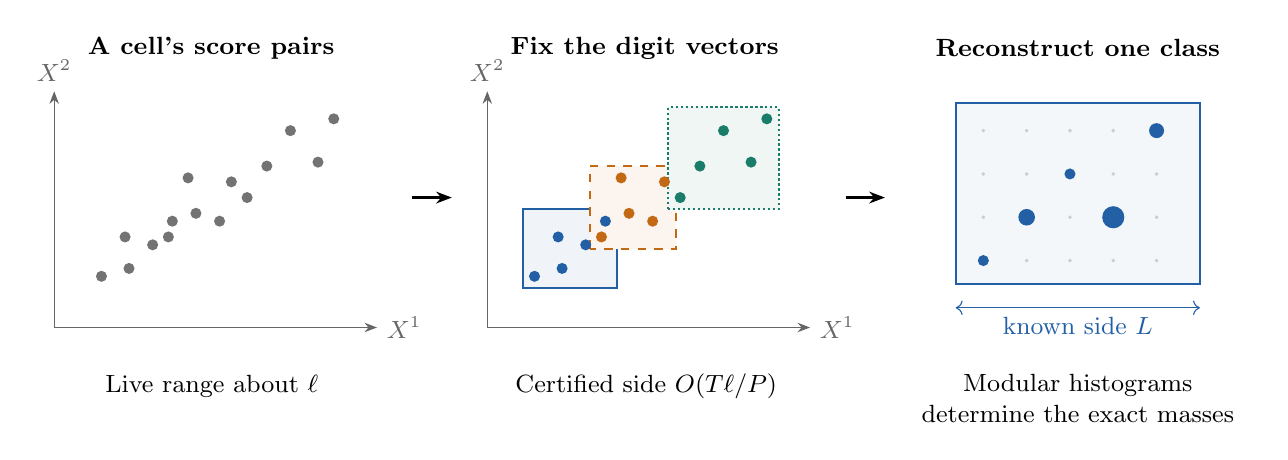
\begin{tikzpicture}[x=1cm,y=1cm,font=\small,
  arr/.style={-{Stealth[length=2mm]},thick},
  axis/.style={-{Stealth[length=1.6mm]},black!60},
  paneltitle/.style={font=\small\bfseries,align=center,text width=4.4cm}]
\definecolor{classblue}{RGB}{35,95,165}
\definecolor{classorange}{RGB}{195,105,20}
\definecolor{classgreen}{RGB}{25,125,105}
\node[paneltitle] at (2,3.55) {A cell's score pairs};
\node[paneltitle] at (7.5,3.55) {Fix the digit vectors};
\node[paneltitle] at (13,3.55) {Reconstruct one class};
\foreach \offset in {0,5.5} {
  \draw[axis] (\offset,0) -- ++(4.1,0) node[right] {$X^1$};
  \draw[axis] (\offset,0) -- ++(0,3) node[above] {$X^2$};
}
\foreach \x/\y in {.6/.65,.95/.75,.9/1.15,1.25/1.05,1.5/1.35,
  1.45/1.15,1.8/1.45,2.1/1.35,1.7/1.9,2.25/1.85,
  2.45/1.65,2.7/2.05,3/2.5,3.35/2.1,3.55/2.65}
  \fill[black!55] (\x,\y) circle (2pt);
\begin{scope}[xshift=5.5cm]
\draw[classblue,fill=classblue!7,thick] (.45,.5) rectangle (1.65,1.5);
\draw[classorange,fill=classorange!7,dashed,thick] (1.3,1) rectangle (2.4,2.05);
\draw[classgreen,fill=classgreen!7,densely dotted,thick] (2.3,1.5) rectangle (3.7,2.8);
\foreach \x/\y in {.6/.65,.95/.75,.9/1.15,1.25/1.05,1.5/1.35}
  \fill[classblue] (\x,\y) circle (2pt);
\foreach \x/\y in {1.45/1.15,1.8/1.45,2.1/1.35,1.7/1.9,2.25/1.85}
  \fill[classorange] (\x,\y) circle (2pt);
\foreach \x/\y in {2.45/1.65,2.7/2.05,3/2.5,3.35/2.1,3.55/2.65}
  \fill[classgreen] (\x,\y) circle (2pt);
\end{scope}
\begin{scope}[xshift=11cm]
\draw[classblue,fill=classblue!5,thick] (.45,.55) rectangle (3.55,2.85);
\foreach \x in {.8,1.35,1.9,2.45,3}
  \foreach \y in {.85,1.4,1.95,2.5}
    \fill[black!20] (\x,\y) circle (.7pt);
\fill[classblue] (.8,.85) circle (2pt);
\fill[classblue] (1.35,1.4) circle (3pt);
\fill[classblue] (1.9,1.95) circle (2pt);
\fill[classblue] (2.45,1.4) circle (4pt);
\fill[classblue] (3,2.5) circle (2.7pt);
\draw[<->,classblue] (.45,.25) -- node[below] {known side $L$} (3.55,.25);
\end{scope}
\draw[arr] (4.55,1.65) -- (5.05,1.65);
\draw[arr] (10.05,1.65) -- (10.55,1.65);
\node[align=center,text width=4.3cm] at (2,-.75)
  {Live range about $\ell$};
\node[align=center,text width=4.3cm] at (7.5,-.75)
  {Certified side $O(T\ell/P)$};
\node[align=center,text width=4.3cm] at (13,-.9)
  {Modular histograms\\determine the exact masses};
\end{tikzpicture}
\caption{Localization followed by reconstruction, schematically.
Each color denotes inputs with one fixed pair of digit vectors.
Their score pairs lie in a certified box; different classes' boxes
can overlap, since digits need not be functions of the scores.
On each known box, modular histograms determine the exact integer
masses once its side fits the reconstruction window.}
\label{fig:localization}
\end{figure}

\subsection{Certify: a bad guess may lose precision, but not soundness}

Concentration shows that useful samples exist. The algorithm cannot
trust that its guessed samples are useful. It checks their ranges
with nonnegative moments. On a cell of \(2^k\) inputs,
\[
 \sum_x v(x)^{2k}<R^{2k}
 \quad\Longrightarrow\quad |v(x)|<R\ \text{for every }x.
\]
A single outlier would exhaust the entire permitted sum. Conversely,
if \(|v(x)|\le R'\) everywhere and \(\sqrt2R'<R\), the test passes.
Thus a constant-factor concentration margin suffices to certify all
points of the cell (\cref{lem:moment}).

The algorithm applies these tests to the digit deviations and to
the score-estimation error, clearing denominators to make the latter
an integer form. A passing cell has two consequences: each digit is
identified by its residue modulo every prime in \((P/2,P]\), and
each fixed digit class has its scores inside an explicit short box.
These consequences use only the tested inequalities and the
telescoping identity; they do not assume that the proposed vectors
were actually sampled.

Passing cells are counted exactly. For a failing cell the counter
reports the whole interval \([0,2^k]\) of possible counts. Summing
these intervals gives a sound global interval for every witness.
The samples are shared across all cells: concentration and averaging
show that one global sampled chain makes almost all cells pass.
That witness gives the required narrow interval
(\cref{prop:sound,prop:complete}).

\subsection{Reconstruct: modular histograms determine a short distribution}

For each prime, we have aggregate residue counts, not residues labeled
by input. Ordinary Chinese remaindering does not identify the
distribution. For example, the two distinct score multisets below
have identical histograms modulo both two and three:
\[
\begin{array}{c|c|c}
 \text{score multiset}&\text{counts at residues }0,1\pmod2
  &\text{counts at residues }0,1,2\pmod3\\ \hline
 \{0,1\}&(1,1)&(1,1,0)\\
 \{3,4\}&(1,1)&(1,1,0).
\end{array}
\]
All four scores lie between zero and five, where an individual
number would be determined by its residues. What is missing is the
matching between those residues. A sufficiently short \emph{known
support interval} restores uniqueness for the histogram.

\paragraph{One score: count the roots.}
Suppose two candidate histograms have the same modular counts and
are supported on the same interval of \(D'\) integers. Translate
that interval to start at zero. The generating polynomial of their
\emph{difference} vanishes at every \(p\)-th root of unity, for each
prime \(p\) used. Distinct primes share only the root one. Hence
there are
\[
 D'=1+\sum_{p\in\mathcal P}(p-1)=\Theta(P^2/\log P)
\]
distinct roots, while the polynomial has degree at most \(D'-1\).
It must be zero (\cref{lem:one-window}).

\paragraph{Two scores: count the factors.}
For two candidates on an \(L\times L\) box, let \(F(u,v)\) be the
generating polynomial of their difference. Project the box onto a
line in a short primitive integer direction. Its projected support
is short enough for the one-score argument, so the projected
difference vanishes. Each such direction forces a distinct
irreducible binomial factor of \(F\), by the method of
Hajdu--Tijdeman~\cite{HT01}. For example,
\[
 F(z,z)=0\ \Longrightarrow\ u-v\mid F,
 \qquad
 F(z,z^{-1})=0\ \Longrightarrow\ uv-1\mid F.
\]
Directions of length up to about \(D'/L\) are usable. Their factors
have total degree of order \((D'/L)^3\) in one variable, whereas
\(F\) has degree less than \(L\) in that variable. There are too
many factors for a nonzero polynomial when \((D'/L)^3\) exceeds a
suitable constant times \(L\). Thus joint modular histograms
uniquely determine any rational-valued histogram on a known box of
side
\[
 L_2=\Theta(D'^{3/4})
    =\Theta\!\left(\frac{P^{3/2}}{(\log P)^{3/4}}\right)
 \qquad\text{(\cref{lem:two-window,lem:window-size}).}
\]
The exact histogram is then recovered by rational linear algebra.

This is the largest possible \emph{power of \(P\)} for arbitrary
box-supported histograms from these measurements. There are
\(\Theta(P/\log P)\) primes, each giving at most \(P^2\) joint
residue counts. Recovering \(L^2\) unrestricted masses therefore
requires \(L^2=O(P^3/\log P)\). Our window matches this dimension
bound up to a factor \((\log P)^{1/4}\) in its side length
(\cref{rem:rank}); this does not limit algorithms that exploit
additional structure of circuit histograms.

The digit tests are what connect this lemma to the algorithm.
On a passing cell, digit residues identify the same actual digit
class across all primes. Restrict the modular tables to that class,
reconstruct its histogram on the certified box, and evaluate the
original lookups against the recovered masses. No smoothness or
other property of the lookups is required.

\subsection{Why the exponent is three}\label{sec:overview-exponent}

The pieces now fit in one inequality. In most cells the live weight
is \(\ell=O(Wk/\sqrt n)\). The certified score width is
\(O(T\ell/P)\), and the two-score reconstruction window has side
\(L_2\). Consequently pair counting succeeds if
\[
 \underbrace{\frac{TWk}{P\sqrt n}}_{\text{localized width}}
 \lesssim
 \underbrace{\frac{P^{3/2}}{(\log P)^{3/4}}}_{\text{reconstruction window}}.
\]
Since \(P\) is near \(n\), and \(T,k\) are logarithmic factors,
the admissible weight is near \(n^3\). Chen--Tal--Wang approximate
the lookup by a probabilistic polynomial of degree
\(\widetilde O(\sqrt\ell)\), allowing live weight near \(n^2\)
under a degree budget below \(n\). Here that budget buys modular
counts and moments; localization plus reconstruction allows live
weight near \(n^{5/2}\). This is the source of the additional
half-power in the gate bound.

\subsection{Why the reconstruction still saves time}\label{sec:overview-cost}

The counter never enumerates the \(2^k\) points of each cell.
Williams' rectangular matrix product, combined with Matou\v{s}ek's
bucketing, computes the required low-degree polynomial sums across
all cells in \(2^{n-k}\operatorname{poly}(n)\) time per table
(\cref{lem:print}; \cite{WilACC14,Mat91}). Fermat tests and
Beigel--Tarui lifting~\cite{BT94} express residue indicators by
such polynomials. Lifting to a modulus \(p^e>2^k\) makes their
summed values exact counts, not just counts modulo \(p\).
Even moments are polynomial sums as well.

The degree budget permits a prime scale
\(P=\Theta(n/(\log n(\log\log n)^2))\). There are
\(J=O(\log\log n)\) sampling stages. The number of modular tables
and digit classes is \(n^{O(\log\log n)}\), which must be paid
for. Each reconstruction solves a system with polynomially many
rows and columns and polynomial-bit arithmetic. The total cost is
therefore
\[
 \underbrace{2^{n-k}}_{\text{cells}}
 \underbrace{n^{O(\log\log n)}}_{\text{tables and reconstruction}}
 \ \le\ \frac{2^n}{n^{\Omega(\log\log n)}},
\]
by choosing the constant in \(k=\Theta(\log n\log\log n)\)
large enough. The proof in \cref{prop:time} fixes this constant
without circular dependence on the other parameters.
The number of guessed sample coefficients is only polynomial;
the larger family of tables is computed by the algorithm.

The exact pair cap, the larger scalar cap, and the dependence on
requested accuracy are stated in \cref{thm:pair-uniform} and proved
in \cref{sec:parameters}. They do not change the polynomial
exponent calculation above.

\subsection{From pair counts to constant-error hardness}\label{sec:overview-transfer}

We now return to the counting-to-hardness connection. A PCP of
proximity replaces a circuit-verification task by local constraints
on encoded input bits and auxiliary proof bits. We use the perfectly
complete three-query construction of Chen--Williams~\cite[Lemma~24]{CW19},
with their linear code and the underlying proximity machinery
of~\cite{BGHSV06}. Its local constraints are ORs of three literals.
Perfect completeness means that a satisfying computation has a proof
meeting every constraint. For a false computation, every proof
violates at least a constant fraction \(\gamma\) of the constraints;
we call \(\gamma\) the \emph{rejection gap}.

The classical MAX-2SAT gadget of
Garey--Johnson--Stockmeyer~\cite{GJS76} replaces a triple by a
quadratic penalty, introducing a Boolean helper \(y\):
\[
 Q(x,y)=1-\sum_i x_i+\sum_{i<j}x_ix_j+2y-y\sum_i x_i.
\]
This is nonnegative on all Boolean assignments and is at least one
on a false triple. For a true triple, \(y^*=x_1x_2x_3\) makes it
zero. For such a true triple \(x\), every Boolean replacement
\(x',y'\) obeys
\[
 Q(x',y')\le\sum_{i=1}^3|x_i-x_i'|+2|y^*-y'|.
\]
Thus the three literal positions have error weight one each, and
the helper has weight two: total weight five. Form the
\emph{weighted local-proof table}. Its inputs are a string \(x\), a
clause index and an address; for each \(x\) and clause it lists the
three queried bits and two copies of the honest helper, each entry
repeated on about a fifth of the addresses. A circuit that errs on a
\(d\) fraction of the table's inputs then incurs mean penalty at most
\((5+\epsilon)d\), for arbitrarily small fixed \(\epsilon>0\).
For each auxiliary proof coordinate, choose its lowest-error table
cofactor and reuse that Boolean circuit at every occurrence;
systematic coordinates remain exact. Weighted occurrence counting
then gives the penalty bound for this one consistent proof assignment.
\Cref{lem:gadget-stability} proves this weighted bound.

The mean penalty is a linear combination of single and pair-XOR
probabilities, using the Boolean identity from
\cref{sec:counting-bridge}. Encoded input bits are explicit parities,
which the counter can also handle. Choosing the appropriate endpoint
of every certified interval gives an upper estimate \(U\) of the
mean penalty, sound for every witness and close to the truth for
some witness. The fast verifier accepts only when \(U\) is below
the proof system's rejection gap \(\gamma\), with a small reserve.

No guessed proof can make a false computation pass. Conversely, a
sufficiently accurate small circuit for the honest weighted local-proof
table would yield an accepting guess. The weight-five bound explains
the error threshold \(d<\gamma/5\). Pair counts suffice because
the entire penalty is quadratic; no three-output counter is needed.
\Cref{sec:gadget-transfer} supplies the exact margins and construction.

\subsection{Why hardness holds at every large length}\label{sec:overview-ae}

The hierarchy construction supplies a fixed hard language; call its
inputs \emph{hierarchy instances}. The fast verifier above is one
fixed nondeterministic machine, which we call the \emph{weak machine}.
It always rejects instances outside that language.
A \emph{refuter} outputs an input on which this machine and the
hierarchy language disagree. Fortnow--Santhanam's hierarchy and the
constructive refuter of Chen--Lyu--Williams~\cite{FS16,CLW20} supply
such an input at every sufficiently large source length. It must therefore
be a true computation that the weak machine rejects on every guess.
Its rejected proof data provide the hard function.

There are two input scales. A hierarchy instance has length \(N\);
the proof-bit functions submitted to the counter have
\(q=\Theta(\log N)\) inputs. To keep this width, the weak machine
guesses a small general circuit describing the source instance and
checks all \(N\) positions. It applies the Murray--Williams
short-PCP interface~\cite{MW20} to the circuit's short
\emph{description}, rather than to the full source word. The
resulting short-PCP verifier has size polynomial in \(q\). Its
\emph{proof oracle} is a table of proof bits queried by address.
The machine also guesses a small circuit for that table and
substitutes it for the oracle. Negating the output, so that \(1\) means
``accept'', gives the \emph{outer verifier}: a circuit on \(q\) inputs
whose input is the short PCP's random string.
The machine then applies the local
proof system and certified counter described above. All guesses
together have polynomial length in \(q\), and the counter's
superpolynomial saving makes the machine fast enough for the refuter.
\Cref{fig:outer-step} gives the full construction.

On the rejected true instance, one of three objects is hard:
\begin{itemize}
\item \textsc{NoSource}: no small general circuit describes the
source word, so that word itself gives a hard truth table.
\item \textsc{NoProof}: the source has a small circuit, but the
first honest outer proof has no small general circuit, so that
proof gives a hard truth table.
\item \textsc{Tautology}: both circuits exist, and substituting them
makes the outer verifier accept every random string. The honest weighted
local-proof table is then hard for the target class: a sufficiently
accurate small circuit for it would make some guess accept.
\end{itemize}
The first two cases use the general-circuit hardness amplification
of Sudan--Trevisan--Vadhan~\cite{STV01}. A target-class circuit of
polynomial top weight has a polynomial-size general-circuit
representation, by integer normalization of its bottom gates and
explicit evaluation of its finite lookup; thus sufficiently strong
general-circuit hardness also excludes the target class.
Canonical choices and padding
turn these cases into one language at every sufficiently large final
length. The language belongs to \(\ENP\) because exponential time
with a SAT oracle suffices to run the refuter, determine the case,
and recover the canonical truth table (\cref{sec:all-lengths}).

\paragraph{Reading the proof.}
\Cref{sec:prelim} states the uniform counting theorem and fixes
notation. \Cref{sec:windows,sec:chains} prove modular reconstruction
and certified localization. \Cref{sec:printing,sec:algorithm,sec:analysis,sec:parameters}
implement and analyze the counter. \Cref{sec:imports,sec:gadget-transfer}
prove the lower-bound transfer, including a common-language refinement
approaching error \(\gamma/5\). The appendices supply supporting
proofs, the source map, machine-model adaptations, and the short-PCP
construction. Apart from the seven published results listed in
\cref{app:formal-boundary}, every step of the main theorem is proved,
in this paper or in its Lean companion; \cref{app:formal-boundary} also
names facts that the paper cites and the companion proves.

\section{The counting interface and mathematical setup}\label{sec:prelim}

This section gives the precise counter guarantee, then fixes the
notation and computational model. Integer normalization, restriction
anti-concentration, and Bernstein's inequality complete the setup.

\subsection{The uniform counting interface}\label{sec:counting-interface}
The full interface makes explicit the accuracy, encoding, and running-time
requirements used by the lower-bound transfer. A call asks for
the acceptance probability of one class circuit \(C^1\), of
\(C^1\oplus C^2\) for two class circuits, or of \(C^1\oplus\PAR_\Sigma\),
where \(\PAR_\Sigma(z)=\bigoplus_{i\in\Sigma}z_i\) is an explicit input parity.
These are exactly the means into which the gadget penalty of
\cref{sec:overview-transfer} decomposes.
Besides the circuits, the algorithm reads a short auxiliary string,
the \emph{witness}, which the weak machine guesses.
\Cref{sec:algorithm} defines the normalized inputs, which have
polynomially bounded integer descriptions; by \cref{lem:integer},
every circuit used later has one.

The pair cap supplies the headline gate exponent. The larger scalar cap
is an additional algorithmic guarantee, not by itself a gate lower bound.
\Cref{sec:parameters} proves both caps with their logarithmic factors.

\begin{theorem}[Uniform certified pair and scalar counting]
\label{thm:pair-uniform}\label{thm:counting}
Fix positive integers \(B_1,B_2\). There is a constant
\(a_{B_1,B_2}>0\) and one algorithm with the following properties. Its
input is a normalized call of total top weight \(W\le2n^4\) together
with a rational requested radius \(n^{-B_1}\le\beta\le1/16\) encoded in
at most \(n^{B_2}\) bits.
Every witness gives a sound probability interval. At every
sufficiently large \(n\), some polynomial-length witness gives radius
at most \(\beta\) if
\[
 W\le a_{B_1,B_2}\beta\mathcal A_3(n),\qquad
 \mathcal A_3(n)=\frac{n^3}{\lambda_n^{21/4}\mu_n^7},
\]
for a pair-XOR call. For a single-circuit or circuit-XOR-raw-parity
call the larger sufficient cap is
\[
 W\le a_{B_1,B_2}\beta\mathcal A_1(n),\qquad
 \mathcal A_1(n)=\frac{n^{7/2}}{\lambda_n^6\mu_n^8}.
\]
For all sufficiently large \(n\), it runs within \(2^n/n^{\mu_n}\) steps,
uniformly over the admitted inputs.
For each prescribed fixed polynomial number of calls, their complete
workload is \(2^n n^{O(1)-\mu_n}\). The algorithm uses no oracle and
reads no guessed data beyond its witness, as the refuter of
\cref{imp:ae-refuter} requires.
\end{theorem}

Soundness for \emph{every} witness lets a verifier guess witnesses
freely, and the superpolynomial saving \(n^{\mu_n}\) in running time pays
for the hierarchy argument.

\subsection{Notation and machine model}

\paragraph{Recurring notation.}
\begin{center}\small
\begin{tabularx}{\textwidth}{@{}>{\raggedright\arraybackslash}p{.30\textwidth}X@{}}
\toprule
\(\lambda_n=\ceil{\lgx n}\), \(\mu_n=\ceil{\lgx\lambda_n}\) & the two logarithmic scales\\
\(\mathcal A_3(n)=n^3/(\lambda_n^{21/4}\mu_n^7)\), \(\mathcal A_1(n)=n^{7/2}/(\lambda_n^6\mu_n^8)\) & pair and scalar caps of \cref{thm:pair-uniform}\\
\(W=W^1+W^2\) & total top weight of the circuits in a call\\
\(k\), \(I\), \(C_y\) & number and set of free (inner) coordinates, \(k=\Theta(\lambda_n\mu_n)\); the cell of outer assignment \(y\)\\
\(\ell^r(y)\) & live weight of circuit \(r\) in cell \(C_y\)\\
\(\beta\); \((\widehat p,\widehat\kappa)\) & requested radius; returned estimate and certified radius\\
\(T\) & concentration parameter, \(\Theta(k)\)\\
\(P\), \(\cP\), \(D'=1+\sum_{p\in\cP}(p-1)\) & prime scale \(\Theta(n/(\lambda_n\mu_n^2))\); the primes in \((P/2,P]\); the one-score window\\
\(L_2\); \(L_w\) & the two-score window \(\Theta(P^{3/2}/\lambda_n^{3/4})\); the window in use, \(L_2\) for pairs and \(D'\) otherwise\\
\(\pi_j\), \(a_j\), \(K_j\), \(E_j\) & sampling rates, their integer ratios, sampled sums, digits (\cref{sec:chains})\\
\(A=\prod_i a_i\), \(M_1=1/\pi_1\), \(\Phi=M_1K_J-AX\) & chain constants and the score test form, \(\pi_J=A/M_1\)\\
\(h\), \(h_E\), \(\Lambda\) & chain height \(\Theta(P)\), digit test threshold \(\floor{P/4}\), score test threshold\\
\(N\), \(q\) & hierarchy source length and PCP width \(q=\Theta(\log N)\) (\cref{sec:imports,sec:gadget-transfer})\\
\(\gamma\), \(Q\) & rejection gap of the three-query PCPP and the gadget penalty (\cref{sec:gadget-transfer})\\
\bottomrule
\end{tabularx}
\end{center}

\paragraph{Machine model.}
Algorithms are deterministic or nondeterministic multitape Turing
machines over a binary alphabet, and time counts machine steps. This is
the model of the imported algorithms (\cref{imp:batch,imp:ae-refuter}).
Arithmetic on polynomial-bit integers uses elementary multiword
algorithms. When an algorithm consults a large table inside a loop, it
first sorts the relevant records by key and then merges, which costs a
logarithmic factor over reading the records once. All such overheads
are fixed polynomial factors.

All logarithms in algorithm parameters are base two; \(\ln\) denotes
the natural logarithm. Empty products are one. For a set
\(I\subseteq[n]\) of size \(k\), write an input as \((y,x)\), where
\(x\in\{0,1\}^I\) and \(y\) assigns the remaining coordinates.
Let
\[
 C_y=\{(y,x):x\in\{0,1\}^I\},\quad z_y=(y,0^I),\quad
 \Delta_y H(y,x)=H(y,x)-H(z_y).
\]
We omit the subscript \(y\) when the cell is fixed. For two circuits,
superscripts \(r=1,2\) distinguish their top sums and gate lists, and
\(W=W^1+W^2\). A sum \(X^r\) can always be expanded as \(W^r\)
signed unit copies of bottom gates. Its live weight \(\ell^r(y)\)
counts the copies whose gates are live. This expansion is used only
in an existence argument; a witness stores one integer coefficient per
gate, rather than individual random choices.

\subsection{Why real bottom weights cause no encoding problem}

The following is a classical integer-normalization fact from threshold
logic~\cite{MTT61}. Only the existence of such a representation
is needed, because circuits are guessed rather than computed.

\begin{lemma}\label{lem:integer}
Every threshold function on \(m\ge1\) Boolean inputs has an equivalent
representation whose weights and threshold are integers in the range
\(\pm m^m\). In particular their bit lengths are \(O(m\log(m+1))\).
\end{lemma}
This is \cite[Lemma~3.2]{CTW26}, attributed there to Muroga, Toda, and
Takasu~\cite{MTT61}. H{\aa}stad~\cite[Section~3]{Has94} gives the sharper
bound \((m+1)^{(m+1)/2}\), by Cramer's rule and Hadamard's inequality; the
weaker bound suffices here.

\subsection{Restrictions and concentration}

The next counting argument is the live-gate estimate in the
restriction method~\cite{KW16}, in the form
of~\cite[Lemma~4.1]{CTW26}. Its chain-counting proof is that
of~\cite[Appendix~A.3]{CTW26}, an instance of Lubell's argument for
Sperner's theorem~\cite{Lub66}.

\begin{lemma}\label{lem:live}
For a threshold gate \(g\), a uniform \(k\)-subset \(I\subseteq[n]\),
and uniform outer assignment \(y\),
\[
 \Pr[g\text{ is live on }C_y]
 \le \frac{k\binom{n-k}{\floor{(n-k)/2}}}{2^{n-k}}
 \le \frac{k}{\sqrt{n-k+1}}.
\]
Consequently, for any collection of circuits of total top weight
\(W\), and any \(\beta>0\), some fixed \(I\) has
\[
 \sum_r\ell^r(y)\le \frac{Wk}{\beta\sqrt{n-k+1}}
\]
on all but a \(\beta\) fraction of cells.
\end{lemma}
The proof specializes the chain-counting argument of
\cite[Appendix~A.3]{CTW26}; it is in \cref{app:live}.

We also use the bounded-variable Bernstein inequality,
Vershynin~\cite[Theorem~2.8.4, first edition]{Vershynin18} with \(K=1\).
\begin{lemma}\label{lem:bernstein}
If independent centered random variables \(Y_t\) satisfy
\(\abs{Y_t}\le1\) and \(\sum_t\E Y_t^2\le V\), then for every \(s>0\),
\[
 \Pr\!\left[\abs{\sum_tY_t}\ge s\right]
 \le2\exp\!\left(-\frac{s^2}{2(V+s/3)}\right).
\]
In particular, for \(T>0\), \(s=\sqrt{2TV}+2T/3\) gives a bound of \(2e^{-T}\).
\end{lemma}
For the particular choice of \(s\), direct expansion gives
\(s^2\ge2T(V+s/3)\).

\section{Recovering distributions from modular counts}\label{sec:windows}

The counter of \cref{sec:printing} will supply exact residue counts of
integer scores. Residues must determine a \emph{distribution}, not just
a single integer. For example, knowing how often a score is even does not
identify which even scores occurred. Our reconstruction lemmas apply
to arbitrary rational-valued functions; positivity is not required.
This permits a clean uniqueness proof by subtracting two candidate
distributions.

Let \(\cP\) be a nonempty finite set of primes and put
\[
 D'=1+\sum_{p\in\cP}(p-1).
\]
For a finitely supported function \(F:\Z^d\to\Q\), define its
modular push-forward by
\[
 F_p(\rho)=\sum_{u\equiv\rho\pmod p}F(u),
 \qquad\rho\in(\Z/p\Z)^d.
\]
Thus \(F_p\) records the total mass of each residue class.

\subsection{One score: a roots-of-unity argument}

\begin{lemma}\label{lem:one-window}
If \(F:\Z\to\Q\) is supported on at most \(D'\) consecutive
integers and \(F_p=0\) for every \(p\in\cP\), then \(F=0\).
\end{lemma}
\begin{proof}
Shift the support to \(\{0,\ldots,D'-1\}\) and form
\(f(t)=\sum_uF(u)t^u\). For every \(p\)-th root of unity \(\zeta\),
\[
 f(\zeta)=\sum_{\rho=0}^{p-1}F_p(\rho)\zeta^\rho=0.
\]
Distinct primes' root sets intersect only at one. Their union therefore
contains \(D'\) distinct roots. A polynomial of degree below \(D'\)
with this many roots is zero.
\end{proof}

\subsection{Two scores: short projections and binomial factors}

Let \(\varphi\) be Euler's totient function and set
\(S(q)=\sum_{m=1}^q m\varphi(m)\), with \(S(0)=0\).
Hajdu and Tijdeman's discrete-tomography method~\cite[Theorem~1 and
its preliminary divisibility lemma]{HT01} turns zero line sums into
binomial divisibility. We prove this over \(\Q\) and count the usable
directions.

\begin{lemma}\label{lem:two-window}
Let \(L\ge2\) and
\(q=\floor{(D'-1)/(L-1)}\). If \(S(q)\ge L\), then a
rational-valued function supported on a given box with both sides at
most \(L\) is uniquely determined, among functions supported on that
box, by its push-forwards \(F_p\), \(p\in\cP\).
\end{lemma}

\emph{Idea of proof.} Take the difference of two functions with the
same data. Each of its projections along a short primitive direction is
a one-score function with zero data, hence zero by the one-score lemma.
Each vanishing projection makes an irreducible binomial divide the
generating polynomial. These binomials have more total degree in one
variable than the polynomial has, so the difference is zero.

\begin{proof}
Subtract two functions with the same data and translate their common
box to \(\{0,\ldots,L-1\}^2\). It suffices to show that a function
with zero data is zero. Write its generating polynomial as
\[
 f(u,v)=\sum_{a,b=0}^{L-1}F(a,b)u^av^b.
\]

\emph{First, every short primitive projection is zero.}
A vector \((\alpha,\beta)\ne(0,0)\) is primitive if
\(\gcd(\abs\alpha,\abs\beta)=1\). If
\(\abs\alpha+\abs\beta\le q\), then
\[
 G(c)=\sum_{\alpha a+\beta b=c}F(a,b)
\]
is supported on an interval containing at most
\((L-1)q+1\le D'\) integers. Its residue data are zero, since
projection commutes with reduction modulo \(p\). By
\cref{lem:one-window}, \(G=0\). Equivalently,
\(f(t^\alpha,t^\beta)=0\) in \(\Q[t,t^{-1}]\).

\emph{Second, each vanishing projection forces a distinct prime factor.}
Choose one vector from each pair \(\pm(\alpha,\beta)\), normalized so
that \(\alpha\ge0\), and \(\beta=1\) if \(\alpha=0\).
The kernel of the substitution \(u\mapsto t^\alpha,v\mapsto t^\beta\)
on \(\Q[u,v]\) is generated by the binomial
\[
 B_{\alpha,\beta}=
 \begin{cases}
 u^\beta-v^\alpha,&\beta\ge0,\\
 u^{\abs\beta}v^\alpha-1,&\beta<0.
 \end{cases}
\]
Here is a direct justification. In the Laurent polynomial ring,
choose integers \(i,j\) with \(\alpha i+\beta j=1\).
The monomials \(\omega_1=u^iv^j\) and \(\omega_2=u^\beta v^{-\alpha}\)
form a coordinate system, because their exponent matrix has
determinant \(-1\). Substitution sends \(\omega_1\) to \(t\) and
\(\omega_2\) to one, so its kernel there is \((\omega_2-1)\). Up to a Laurent monomial unit, this is
the displayed binomial. That binomial has no factor \(u\) or \(v\).
It is irreducible in \(\Q[u,v]\): a factorization gives a Laurent
unit factor, since \(\omega_2-1\) is irreducible in the Laurent ring,
hence a monomial, which must be constant.
Clearing Laurent denominators and using unique factorization gives
the asserted polynomial kernel.

Nonparallel primitive directions give nonassociate binomials:
substitution in the other direction gives two powers of \(t\)
whose exponents differ by \(\pm(\alpha\beta'-\beta\alpha')\ne0\).
By unique factorization, the product of these binomials divides \(f\).

\emph{Finally, there are too many factors for a nonzero \(f\).}
The sum of their degrees in \(u\) is
\(\sum\abs\beta\), over primitive directions modulo sign of norm
at most \(q\). At norm one, the horizontal and vertical directions
contribute one in total. At norm \(m\ge2\), the directions contribute
\[
 2\sum_{\substack{1\le a<m\\\gcd(a,m)=1}}(m-a)
 =m\varphi(m),
\]
using the symmetry \(a\leftrightarrow m-a\). Thus the product has
\(u\)-degree \(S(q)\ge L\), whereas \(\deg_uf\le L-1\).
This is impossible unless \(f=0\).
\end{proof}

For a concrete picture, the projection \((\alpha,\beta)=(1,1)\)
adds masses along diagonals \(a+b=c\). If all those sums vanish,
\(u-v\) divides \(f\). The projection \((1,-1)\) instead forces
\(uv-1\). The lemma uses many such independent factors, not just
the coordinate projections.

\begin{lemma}\label{lem:window-size}
For every integer \(q\ge1\),
\[
 S(q)\ge\frac{2q^3}{\pi^2}-q^2(4/3+\ln q).
\]
Call \(L\ge2\) admissible if \(S(\floor{(D'-1)/(L-1)})\ge L\), as in
\cref{lem:two-window}. Let \(L_2\) be the largest admissible \(L\),
or one if none exists. Then
\(L_2=\Theta(D'^{3/4})\) as \(D'\to\infty\).
In particular \(L_2\ge\floor{(3/5)D'^{3/4}}\) for all sufficiently
large \(D'\).
\end{lemma}
The proof is a standard totient-summation calculation, given in
\cref{app:window-size}.

Uniqueness also gives an algorithm: introduce one rational unknown
per box point and one equation per residue class. The matrix entries
are zero or one. Exact Gaussian elimination finds the unique
distribution whenever the data come from a function on the box.
An algorithm may also detect inconsistency and report uncertainty.
A box with one point is determined by its total mass, so the
singleton convention in the definition of \(L_2\) is also sound.

\subsection{How many useful primes are available?}

For an integer \(P\ge3\), let \(\cP\) consist of all primes in
\((P/2,P]\). Only the order of magnitude of this set is needed.

\begin{lemma}\label{lem:primes}
For this prime set, as \(P\to\infty\),
\[
 D'=\Theta(P^2/\ln P),\qquad
 L_2=\Theta\!\left(P^{3/2}/(\ln P)^{3/4}\right).
\]
\end{lemma}
\begin{proof}
By the prime number theorem~\cite[Chapters~4 and~13]{Apostol76}, the
interval \((P/2,P]\) contains \((1+o(1))P/(2\ln P)\) primes;
Erd\H{o}s' elementary argument for Bertrand's postulate~\cite{Erdos32}
already gives this order of magnitude. Each such prime contributes
more than \(P/2-1\) and at most \(P\) to \(D'\), so
\(D'=\Theta(P^2/\ln P)\). Apply \cref{lem:window-size}.
\end{proof}

\begin{remark}[The limitation of full-box residue reconstruction]\label{rem:rank}
For distributions on \(\{0,\ldots,L-1\}^d\), the residue map has
rank at most \(1+\sum_{p\in\cP}(p^d-1)\): all primes report the
same total mass. Injectivity therefore requires
\(L^d\le1+\sum_p(p^d-1)\).
For two scores this yields
\(L=O(P^{3/2}/\sqrt{\ln P})\). Our box bound has the same power
of \(P\), with an additional factor \((\ln P)^{1/4}\) loss.
This is a restriction on recovering \emph{arbitrary} box-supported
distributions from these data, not an impossibility theorem for all
circuit-analysis methods or for more structured distributions.
\end{remark}

\section{Nested subsampling produces short integer digits}\label{sec:chains}

We now turn a potentially large live sum into short forms that can
be identified from one residue. Sampling at a single very small rate
would make the first sampled sum short, but leave a poor estimate of
the original sum. The chain increases the rate while keeping each
new correction short. Integer rate ratios preserve exact arithmetic.

\begin{lemma}[Choice of rates]\label{lem:chain}
Let \(T>0\), let \(h\) be an integer with \(h\ge64T\), and let
\(\ell_0\ge0\). Define
\[
 \bar\ell=\max\{\ell_0,h^2/(256T)\},\quad
 \pi^*=\frac{h^2}{8T\bar\ell},\quad
 s(\pi)=\sqrt{2T\pi\bar\ell}+\frac{2T}{3},
\]
\[
 M_1=\ceil{4\bar\ell/h},\qquad \pi_1=1/M_1.
\]
While \(x_j=\pi_j/\pi^*<2^{-8}\), set
\[
 a_j=\floor{1/(4\sqrt{x_j})},\qquad \pi_{j+1}=a_j\pi_j.
\]
Stop at the first index \(J\) with \(x_J\ge2^{-8}\). Then
\begin{enumerate}[label=(\roman*)]
\item \(a_j\ge4\), all rates lie in \((0,1]\), and
\(\pi_j=\prod_{i<j}a_i/M_1\).
\item \(\pi_1\bar\ell+s(\pi_1)\le h/2\), and
\(s(\pi_{j+1})+a_js(\pi_j)\le h/2\) for \(j<J\).
\item \(J\le\ceil{\lgx\lgx(h/T)}+1\).
\item \(s(\pi_J)/\pi_J\le86T\bar\ell/h\).
\end{enumerate}
\end{lemma}
\begin{proof}
Since \(h\ge64T\), the second entry of the maximum gives
\(\bar\ell\ge h^2/(256T)\ge h/4\).
Thus \(4\bar\ell/h\le M_1\le8\bar\ell/h\), and
\[
 T/h\le x_1\le2T/h\le1/32.
\]
Write \(\tau(\pi)=\sqrt{2T\pi\bar\ell}
=(h/2)\sqrt{\pi/\pi^*}\).
For the first digit,
\(\pi_1\bar\ell\le h/4\),
\(\tau(\pi_1)\le\sqrt{Th/2}\le h/8\), and \(2T/3\le h/96\).

During a step, \(a_j\ge4\),
\(a_j\sqrt{x_j}\le1/4\), and
\(a_jx_j\le\sqrt{x_j}/4\), so \(\sqrt{a_jx_j}\le x_j^{1/4}/2<1/8\). Consequently
\[
 \tau(\pi_{j+1})+a_j\tau(\pi_j)
 =\frac h2\bigl(\sqrt{a_jx_j}+a_j\sqrt{x_j}\bigr)
 \le\frac{3h}{16}.
\]
The \(x_j\) increase, so
\(a_j\le\sqrt{h/T}/4\), and
\[
 (1+a_j)\frac{2T}{3}
 \le h/96+\sqrt{hT}/6\le h/32.
\]
These bounds prove (ii).
Every newly produced \(x_{j+1}\) is below \(1/64\), while
\(x_1\le1/32\). Also \(\pi^*\le32\), so all rates are at most one.

Since \(1/(4\sqrt{x_j})>4\) during a step, flooring loses at most
a factor two, and
\(x_{j+1}\ge\sqrt{x_j}/8\).
For \(y_j=\lgx(1/x_j)\), this means
\(y_{j+1}-6\le(y_j-6)/2\).
If the chain has not stopped earlier, iteration gives
\(y_j\le6+2^{-(j-1)}y_1\), with
\(y_1\le\lgx(h/T)\). A step at index \(j\) requires \(y_j>8\), hence
\(2^{j-1}<y_1/2\) and \(j<\lgx y_1\). Applied to \(j=J-1\) when
\(J\ge2\), this gives \(J<\lgx\lgx(h/T)+1\), which proves (iii).
At the stopping index, \(x_J\ge2^{-8}\), so
\(\pi_J\ge h^2/(2048T\bar\ell)\); with \(T/h\le1/64\) this gives
\[
 \frac{s(\pi_J)}{\pi_J}
 \le\frac{64T\bar\ell}{h}
       +\frac{1366T^2\bar\ell}{h^2}
 \le\frac{86T\bar\ell}{h}.
\]
This proves (iv) and completes the argument.
\end{proof}

Expand a top sum \(X\) into signed unit copies \(\sigma_tg_{i(t)}\).
Choose independent uniform \(u_t\in[0,1]\) and define
\[
 K_j=\sum_t\ind[u_t\le\pi_j]\sigma_tg_{i(t)},\qquad
 E_0=K_1,\quad E_j=K_{j+1}-a_jK_j\ (1\le j<J).
\]
Let
\[
 A=\prod_{i=1}^{J-1}a_i,\qquad A_0=A,\qquad
 A_j=\prod_{i=j+1}^{J-1}a_i\quad(1\le j<J).
\]
The identities
\begin{equation}\label{eq:telescope}
 K_J=\sum_{j=0}^{J-1}A_jE_j,\qquad \pi_J=A/M_1
\end{equation}
follow by repeatedly substituting \(K_{j+1}=a_jK_j+E_j\).
The first identity holds for \emph{any} proposed coefficient vectors
\(K_1,\ldots,K_J\), whether or not they arose from nested sampling.
That fact will be essential for soundness.

\begin{lemma}[A good sampled chain inside one cell]\label{lem:sampled}
If a cell has live weight at most \(\ell_0\), then, with probability
at least \(1-2J2^ke^{-T}\), simultaneously for every point of the
cell and every stage,
\[
 \abs{\Delta K_j-\pi_j\Delta X}\le s(\pi_j).
\]
On this event,
\[
 \abs{\Delta E_j}\le h/2\quad(0\le j<J),\qquad
 \abs{\Delta K_J-\pi_J\Delta X}\le s(\pi_J).
\]
On a class with fixed digit vector \(E=\kappa\), the score \(X\)
then lies in an interval with at most
\(2s(\pi_J)/\pi_J+1\) integer values.
\end{lemma}
\begin{proof}
For a fixed point and stage, the error is
\[
 \sum_t(\ind[u_t\le\pi_j]-\pi_j)\sigma_t
             (g_{i(t)}(y,x)-g_{i(t)}(z_y)).
\]
The summands are independent, centered, and bounded by one.
Only live copies contribute, each with variance
\(\pi_j(1-\pi_j)\le\pi_j\), and there are at most \(\ell_0\le\bar\ell\)
of them. Thus the total variance is at most
\(\pi_j\bar\ell\). Apply \cref{lem:bernstein} and take a union bound
over the \(2^k\) points and \(J\) stages. Duplicate copies of the
same gate do not impair independence: their gate differences are
fixed coefficients, and their \(u_t\)'s are independent.

For \(E_0\), use \(\abs{\Delta X}\le\ell_0\le\bar\ell\), since only live
copies change, and
\cref{lem:chain}(ii). For later digits the mean terms cancel, since
\(\pi_{j+1}=a_j\pi_j\); the error is the difference of two stage
errors with coefficients one and \(-a_j\). The same part of the
chain lemma applies. Finally \eqref{eq:telescope} fixes \(K_J\)
on a digit class, and the last stage's error bounds \(\pi_JX\)
in an interval of length \(2s(\pi_J)\).
\end{proof}

The digits need not be functions of \(X\). Two inputs may have the
same total score while different sampled contributions fire.
We condition on the digits themselves, not on score level sets.

\subsection{Even moments certify arbitrary proposals}

The following elementary moment bound is the pointwise certification
device. The moment method and Markov's inequality are standard; the
role here is to certify a globally proposed chain using operations
that the polynomial tabulator of \cref{sec:printing} can perform.

\begin{lemma}\label{lem:moment}
Let \(k\ge1\), \(v:\{0,1\}^k\to\Z\), and \(R\ge1\) be an integer.
If \(\sum_xv(x)^{2k}<R^{2k}\), then \(\abs{v(x)}<R\) everywhere.
Conversely, if \(\abs{v(x)}\le R'\) everywhere and
\(\sqrt2R'<R\), then the same moment inequality holds.
\end{lemma}
\begin{proof}
One value of magnitude at least \(R\) would contribute at least
\(R^{2k}\). Conversely the sum is at most \(2^k(R')^{2k}<R^{2k}\).
\end{proof}

\section{What the fast algorithm can count}\label{sec:printing}

This section assembles established exact-threshold and polynomial
tools into the tabulation operation used later. ``Tabulate'' means
compute one answer for \emph{every} outer assignment \(y\), in time
\(2^{n-k}\) times a polynomial factor. It does not mean evaluating
all \(2^k\) points separately inside every cell.

\subsection{Thresholds as disjoint exact tests}

An exact threshold gate is \(\ind[u(z)=0]\) for an integer affine
form \(u\). Hansen and Podolskii~\cite[Theorem~7]{HP10} established polynomial-size
disjoint exact-threshold representations, and Chen and
Williams~\cite[Proposition~18(2) and Appendix~B, Lemmas~48--49]{CW19} gave a more
efficient first-crossing construction. We need only the following
conservative bound; its proof (\cref{app:exact}) records a
bounded-remainder encoding that makes all bit lengths explicit.

\begin{lemma}\label{lem:exact}
Let \(g\) be a threshold gate on \(m\ge1\) inputs with integer weights
and threshold of magnitude below \(2^{B'}\). Put
\[
 B_b=B'+\ceil{\lgx(m+1)}+1,\qquad
 m_T=1+B_bm\ceil{m/2}.
\]
Then \(g\) is a sum of at most \(m_T\) exact threshold indicators,
at most one of which is one on any input. Their affine coefficients
have bit length \(O(B'+\log(m+1))\).
\end{lemma}

Two other standard facts are worth making explicit; the first is
\cite[Proposition~18(5)]{CW19}.
If integer affine forms \(u_1,\ldots,u_d\) have
\(\abs{u_i(z)}\le R\) on the cube, then
\[
 \bigwedge_{i=1}^d[u_i(z)=0]
 \quad\Longleftrightarrow\quad
 \sum_{i=1}^d(R+1)^{i-1}u_i(z)=0.                 \tag{*}\label{eq:pack}
\]
Indeed, if \(i_0\) is the first index with \(u_{i_0}(z)\ne0\), the sum
is \((R+1)^{i_0-1}\) times an integer congruent to
\(u_{i_0}(z)\not\equiv0\) modulo \(R+1\).
The packed coefficients use \(O(d\log(R+1))\) bits. Moreover,
\(\ind[u=0]=\ind[u\ge0]-\ind[u\ge1]\).
These observations explain why signed sums, rather than just Boolean
outputs, are useful.

\subsection{The published rectangular product and signed printing}

The fast tabulation uses one published algorithm, Williams' uniform
rectangular matrix multiplication.

\begin{import}[Williams]\label{imp:batch}
There is one deterministic multitape Turing machine that, for all
sufficiently large \(N\), multiplies over the integers any two
\(0\)-\(1\) matrices of dimensions \(N\times\ceil{N^{0.1}}\) and
\(\ceil{N^{0.1}}\times N\) in \(N^2\poly(\log N)\) steps.
\end{import}

This is \cite[Corollary~4.4, restated as Corollary~C.2]{WilACC14}. In
its Appendix~C, Williams verifies that Coppersmith's rectangular
algorithm~\cite{Cop82} is uniform and can be implemented, ``even on a
multitape TM,'' within this time. The same import underlies
\cite[Appendix~B]{NagCubic}. Williams' weighted threshold
product~\cite[Theorem~3.1]{Wil14} would allow up to \(N^{1/12}\) gates
on all \(N^2\) points of \(A\times B\) with \(\abs A=\abs B=N\); we derive the smaller allowance we need from \cref{imp:batch}
instead, so that the only imported algorithm is a multitape matrix
product. The next two lemmas follow \cite[Appendix~B]{NagCubic}: binary
slicing handles signed entries, and Matou\v{s}ek's bucketing~\cite{Mat91}
reduces weighted dominance to rectangular products.

\begin{lemma}[Signed-by-Boolean product]\label{lem:signed-boolean-product}
Fix a constant \(\nu\ge1\). Let \(1\le d\le\ceil{u^{0.1}}\),
\(A\in\Z^{u\times d}\) and \(B\in\{0,1\}^{d\times u}\), with
\(\abs{A_{ij}}<2^b\) and \(b\le(\lgx(u+2))^\nu\). Then the integer
product \(AB\) is computable in \(u^2\poly(\log u)\) steps.
\end{lemma}
\begin{proof}
For \(0\le t<b\), let \(A_t^+\) contain the \(t\)th magnitude bit of
every positive entry of \(A\), and let \(A_t^-\) contain the \(t\)th
magnitude bit of every negative entry. Both matrices are Boolean, and
\(A=\sum_{t<b}2^t(A_t^+-A_t^-)\); hence
\(AB=\sum_{t<b}2^t(A_t^+B-A_t^-B)\). Zero-pad the common dimension to
\(\ceil{u^{0.1}}\) and apply \cref{imp:batch} to the
\(2b=\poly(\log u)\) Boolean products. A bit-plane product entry lies in
\([0,d]\), so a recombined entry has at most
\(b+\ceil{\lgx(d+1)}+1=\poly(\log u)\) bits. Constructing the zero-padded planes
costs \(u\ceil{u^{0.1}}b\poly(\log u)\), and recombination at all \(u^2\) entries costs
\(u^2\poly(\log u)\). Values of \(u\) below the imported onset are handled
directly.
\end{proof}

\begin{lemma}[Signed exact-threshold printing]\label{lem:signed-printer}
Fix a constant \(c\ge1\). For every sufficiently large \(r\), let
\(G_i(z)=\ind[\ell_i(z)=\theta_i]\), \(1\le i\le s\), be exact threshold
gates on \(r\) Boolean variables whose integer weights and thresholds
have bit length at most \(r^c\), and let \(v_1,\ldots,v_s\) be integers
of bit length at most \(r^c\). If \(s\le2^{r/100}\), the complete table
\[
 z\longmapsto\sum_{i=1}^sv_iG_i(z),\qquad z\in\{0,1\}^r,
\]
can be printed in \(2^r\poly(r)\) steps.
\end{lemma}

\emph{Idea of proof.} Write each exact threshold as a difference of two
ordinary thresholds. Split the input into two halves. An ordinary
threshold then compares a value computed from the left half with one
computed from the right half, so the table is a weighted dominance
matrix. Matou\v{s}ek's bucketing counts the comparisons within a bucket
directly. It turns all the others into one rectangular product of a
signed matrix and a Boolean matrix, which the preceding lemma computes.

\begin{proof}
Replace every equality by two weak cuts,
\(\ind[\ell=\theta]=\ind[\ell\ge\theta]-\ind[\ell\ge\theta+1]\). The table
becomes a signed sum \(\sum_{j=1}^{s'}\omega_jH_j(z)\) of \(s'\le2s\)
threshold gates, whose coefficients are the integers \(\pm v_i\).

First let \(r=2d'\) be even, split \(z=(a,b)\) into two \(d'\)-bit
halves, and put \(N_h=2^{d'}\). Write the linear form of \(H_j\) as
\(\ell_j^{\rm L}(a)+\ell_j^{\rm R}(b)\) with threshold \(\theta_j\), and
define \(A[a,j]=\theta_j-\ell_j^{\rm L}(a)\) and
\(B[j,b]=\ell_j^{\rm R}(b)\). Then \(H_j(a,b)=\ind[A[a,j]\le B[j,b]]\), so
the desired table is the weighted dominance matrix
\begin{equation}\label{eq:dominance}
 \mathsf P[a,b]=\sum_{j=1}^{s'}\omega_j\ind[A[a,j]\le B[j,b]].
\end{equation}
Put \(\delta=0.049\). Since \(s'\le2^{r/100+1}=2N_h^{0.02}\le N_h^\delta\)
eventually, pad the gate index to \(\ceil{N_h^\delta}\) gates with zero
coefficients. For each \(j\), sort together the \(N_h\) values
\(A[a,j]\) and the \(N_h\) values \(B[j,b]\), placing every \(A\) copy
before every equal \(B\) copy. Then \(A[a,j]\le B[j,b]\) exactly when the
former precedes the latter. Partition each sorted list into consecutive
buckets of at most \(\ceil{N_h^{1-\delta}}\) entries. For every pair
\((a,j)\), scan the \(B[j,b]\) entries in the bucket of \(A[a,j]\) and add
\(\omega_j\) for each correctly ordered pair. This inspects at most
\(N_h\ceil{N_h^\delta}\ceil{N_h^{1-\delta}}=O(N_h^2)\) pairs.

Every other correctly ordered pair has its \(B\) entry in a later bucket.
With \(h\) ranging over bucket labels, put
\begin{gather*}
 A'[a,(j,h)]=\begin{cases}\omega_j,&A[a,j]\text{ lies in bucket }h,\\
 0,&\text{otherwise},\end{cases}\\
 B'[(j,h),b]=\ind[\text{the bucket of }B[j,b]\text{ is later than }h].
\end{gather*}
Each sorted list has at most \(2N_h^\delta+1\) buckets, so the common
dimension is \(O(N_h^{2\delta})=O(N_h^{0.098})\le\ceil{N_h^{0.1}}\) for
large \(N_h\). The left matrix has signed entries of \(\poly(r)\) bits and
the right matrix is Boolean, so \cref{lem:signed-boolean-product} with
\(u=N_h\) computes \(A'B'\) exactly. Its \((a,b)\) entry is the
contribution of later buckets; adding the same-bucket contribution gives
\eqref{eq:dominance} exactly.

Sorting costs \(N_h^{1+\delta}\poly(r)\). Writing out \(A'\) and \(B'\), each with \(O(N_h^{1+2\delta})\) entries, costs \(N_h^{1+2\delta}\poly(r)\le N_h^{1.1}\poly(r)\), and every
table entry is a sum of \(O(N_h^{0.098})\) coefficients of \(\poly(r)\)
bits. With the \(O(N_h^2)\) same-bucket pairs and the \(N_h^2\poly(r)\) product of \cref{lem:signed-boolean-product}, the total is \(N_h^2\poly(r)=2^r\poly(r)\) steps. If \(r\) is odd,
add one ignored variable, run the even case, and keep the slice where it
is zero.
\end{proof}

In particular, a signed sum of at most \(2^{m/100}\) exact-threshold
indicators on \(m\) variables, with polynomial-bit parameters and
coefficients, can be tabulated in \(2^m\poly(m)\) time.

\begin{lemma}[Polynomial tabulation]\label{lem:print}
Consider \(G=\poly(n)\) threshold gates on \(n\) inputs with
polynomial-bit integer parameters. Fix \(k<n\) inner coordinates,
and let \(m\) be \(n-k\) rounded up to an even integer.
Let \(Q\) be an integer multilinear polynomial of degree at most
\(D\) in \(G''\le2G\) formal variables, each standing for either
\(g_i(y,x)\) or \(g_i(y,0^I)\). Its coefficients have polynomial bit
length. It may be supplied explicitly, or expanded from a polynomial-size
arithmetic formula of formal degree at most \(D\) with polynomial-bit
intermediate coefficients.
Let \(m_T\) be the bound of \cref{lem:exact} for gates on \(n-k\)
inputs whose integer parameters have magnitude below \(2^{B'}\), where
\(B'\) is the original bit-length bound plus \(\ceil{\lgx(n+1)}+1\). If
\begin{equation}\label{eq:print-condition}
 k+2+D\lgx(1+G''m_T)\le m/100,
\end{equation}
then all integers \(\sum_{x\in H}Q(y,x)\) can be tabulated in
\(2^{n-k}n^{O(1)}\) time, for any fixed subset
\(H\subseteq\{0,1\}^I\). The polynomial overhead is uniform when
all bit-length bounds and \(D\) are bounded by fixed polynomials in \(n\).
\end{lemma}
\begin{proof}
Fix \(x\). Each polynomial variable is a threshold gate on \(y\);
fixing the inner coordinates increases its parameter bit length by
at most \(\ceil{\lgx(n+1)}+1\). Replace it by the disjoint sum in
\cref{lem:exact}. Expand a degree-\(d\) monomial and pack each
conjunction by \eqref{eq:pack}. The result is a signed sum of at most
\(m_T^d\) exact-threshold indicators. Summing over \(x\in H\), where
\(\abs H\le2^k\), gives at most
\[
 2^{k}\sum_{d\le D}\binom{G''}{d}m_T^d
 \le2^{k}(1+G''m_T)^D\le2^{m/100-2}
\]
indicators. The binomial-sum inequality also holds for \(D=0\);
for \(D\ge1\), compare each coefficient with the expansion of
\((1+G''m_T)^D\). All packed parameters have polynomial bit length.

Dense polynomial expansion costs at most
\((1+G'')^{2D}n^{O(1)}\le2^{m/50}n^{O(1)}\), and constructing the
threshold list is cheaper than the final tabulation bound. Apply
\cref{lem:signed-printer} on the full cube of \(m\) variables. If a dummy
variable was added, its two slices are identical; keep one slice.
This changes time by a factor of at most two.
\end{proof}

\subsection{Fermat tests and Beigel--Tarui lifting}

The next amplifier is due to Beigel and Tarui~\cite{BT94}, building on
earlier modulus-amplification work of Toda and Yao~\cite{Tod91,Yao90}. It is also the
amplifier used in Williams' ACC analysis~\cite{WilACC14}.
\begin{lemma}\label{lem:amp}
For \(e\ge1\), define
\[
 \Amp_e(t)=1-(1-t)^e\sum_{j=0}^{e-1}\binom{e-1+j}{j}t^j.
\]
This integer polynomial has degree \(2e-1\), with
\(t^e\mid\Amp_e(t)\) and \((1-t)^e\mid1-\Amp_e(t)\).
Consequently, modulo \(p^e\), it maps an integer congruent to zero
modulo \(p\) to zero, and one congruent to one to one.
\end{lemma}
This is the modulus-amplifying polynomial of Beigel and
Tarui~\cite[Section~2.3]{BT94}.
\begin{proof}
The power-series identity
\((1-t)^{-e}=\sum_{j\ge0}\binom{e-1+j}{j}t^j\) shows that truncating
at degree \(e-1\) leaves an error divisible by \(t^e\).
Multiplication by \((1-t)^e\) proves the first divisibility assertion.
The second is immediate from the definition. Both imply the stated
congruences, including for negative integer arguments.
\end{proof}

\begin{lemma}[Exact joint residue counts]\label{lem:residue-count}
Let \(L_1,\ldots,L_r\) be integer affine forms in the gate outputs,
let \(p\) be prime, let \(e\ge1\) be an integer, and let
\(\rho\in(\Z/p\Z)^r\), with each \(\rho_i\) represented in
\(\{0,\ldots,p-1\}\). If \(p^e>2^k\),
the Boolean multilinearization of
\[
 Q_{p,\rho}
 =\Amp_e\!\left(\prod_{i=1}^r
              \bigl(1-(L_i-\rho_i)^{p-1}\bigr)\right)
\]
has degree at most \((2e-1)r(p-1)\), and
\[
 \#\{x\in H:L_i(y,x)\equiv\rho_i\pmod p\text{ for all }i\}
 =\left(\sum_{x\in H}Q_{p,\rho}(y,x)\right)\bmod p^e.
\]
The remainder is taken in \(\{0,\ldots,p^e-1\}\).
\end{lemma}
\begin{proof}
Fermat's theorem makes each factor an indicator modulo \(p\).
Their product is zero or one modulo \(p\), and \cref{lem:amp} lifts
it to the corresponding indicator modulo \(p^e\). Replacing every
positive power of a Boolean variable by its first power preserves
its values and cannot increase degree. The actual count is at most
\(2^k<p^e\), so there is no ambiguity in the remainder.
\end{proof}

\section{A counting algorithm that certifies every guess}\label{sec:algorithm}

The algorithm has three allowed inputs:
one class circuit \(C^1\); two circuits with predicate
\(C^1\oplus C^2\); or one circuit with predicate
\(C^1\oplus\PAR_\Sigma\), where
\(\PAR_\Sigma(z)=\bigoplus_{i\in\Sigma}z_i\).
The last form keeps an input parity explicit rather than paying for
an unnecessary second class circuit.

We restrict the completeness and running-time analysis to the
encodings that the lower-bound argument uses. On \(n\ge4\) inputs,
let
\[
 G_0=2n^4,\qquad B_0=4n\ceil{\lgx(n+1)}.
\]
A \emph{normalized call} has total top weight \(W\le2n^4\), hence at
most \(G_0\) bottom gates (gates of top weight zero are discarded),
and integer bottom parameters of magnitude
below \(2^{B_0}\). Each \(f^r\) is given as a table on
\([-W^r,W^r]\cap\Z\). The entire encoding has polynomial length.
By \cref{lem:integer}, all circuit representations needed later can
be guessed in this form. A wrapper may return \((1/2,1/2)\) on other
valid encodings without claiming a useful estimate for them.

Fix positive integers \(B_1,B_2\). The input includes a rational
requested radius \(\beta\) satisfying \(n^{-B_1}\le\beta\le1/16\), whose
encoding uses at most \(n^{B_2}\) bits. Failed public precision or encoding
guards return the sound default. The fixed reserve \(c_T\) of
\cref{sec:finite} may depend on \(B_1,B_2\). The algorithm returns dyadic rationals
\((\phat,\khat)\) with
\(\abs{\phat-\Pr[C(z)=1]}\le\khat\).
Its proposed auxiliary data are called the \emph{witness}; it is
guessed when we use the algorithm nondeterministically.

\begin{figure}[t]
\centering
\resizebox{\linewidth}{!}{%
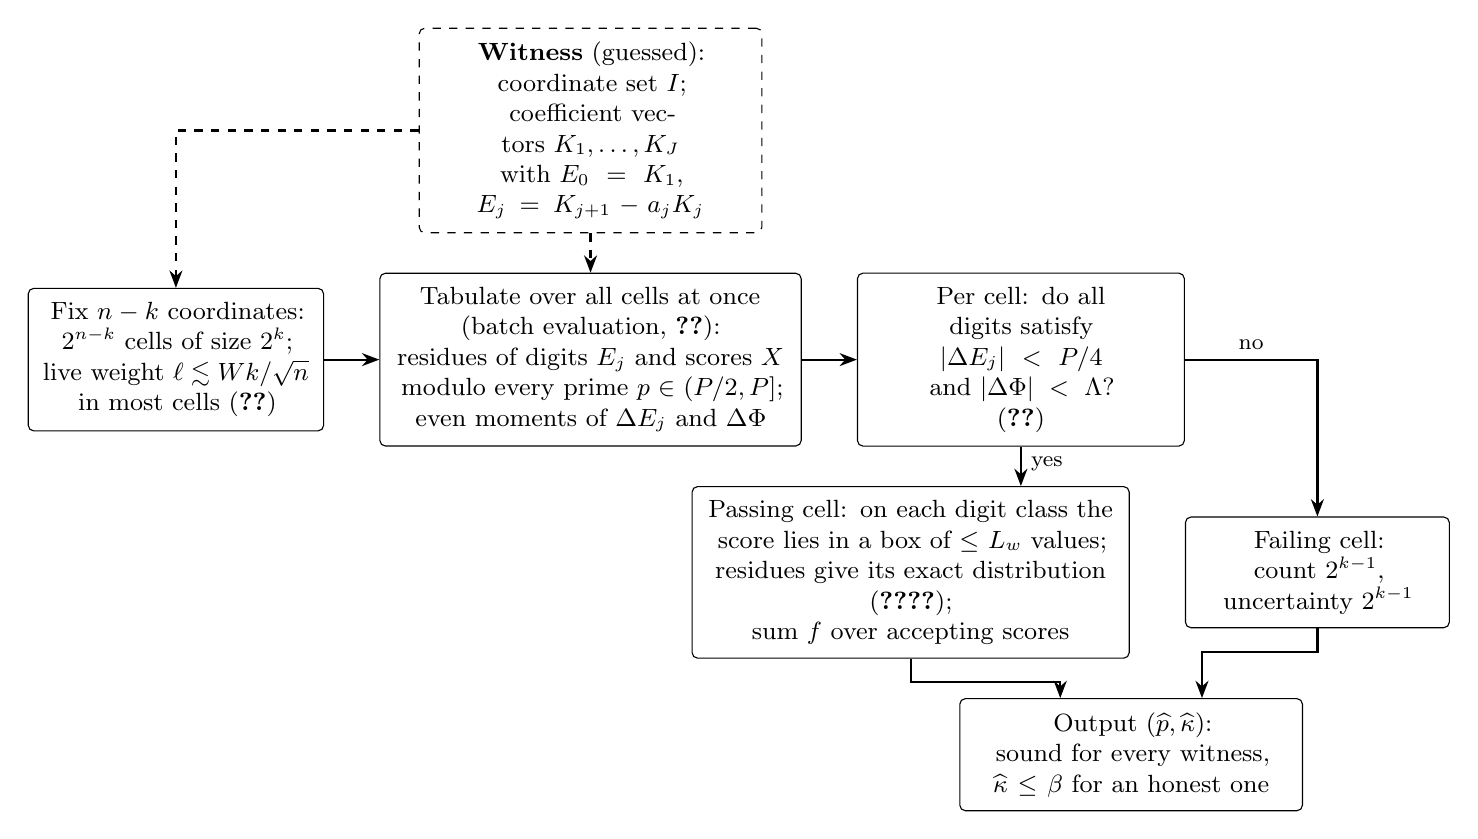
\begin{tikzpicture}[
  font=\small,
  box/.style={draw,rounded corners=2pt,align=center,inner sep=5pt,
              minimum height=11mm,text width=#1},
  wit/.style={draw,dashed,rounded corners=2pt,align=center,inner sep=5pt,
              text width=#1},
  arr/.style={-{Stealth[length=2.2mm]},thick},
  lab/.style={font=\footnotesize,align=center},
  node distance=5mm and 7mm]
\node[box=34mm] (cells) {Fix $n-k$ coordinates:\\ $2^{n-k}$ cells of size $2^k$;\\
  live weight $\ell\lesssim Wk/\sqrt n$\\ in most cells (\cref{lem:live})};
\node[box=50mm,right=of cells] (tab) {Tabulate over all cells at once\\
  (batch evaluation, \cref{lem:print}):\\
  residues of digits $E_j$ and scores $X$\\ modulo every prime $p\in(P/2,P]$;\\
  even moments of $\Delta E_j$ and $\Delta\Phi$};
\node[box=38mm,right=of tab] (test) {Per cell: do all digits satisfy\\
  $\abs{\Delta E_j}<P/4$ and $\abs{\Delta\Phi}<\Lambda$?\\
  (\cref{lem:moment})};
\node[box=52mm,below=of test,xshift=-14mm] (rec) {Passing cell: on each digit class the\\
  score lies in a box of $\le L_w$ values;\\
  residues give its exact distribution\\
  (\cref{lem:one-window,lem:two-window});\\ sum $f$ over accepting scores};
\node[box=30mm,right=of rec] (fail) {Failing cell:\\ count $2^{k-1}$,\\ uncertainty $2^{k-1}$};
\node[box=40mm,below=of rec,xshift=28mm] (out) {Output $(\widehat p,\widehat\kappa)$:\\
  sound for every witness,\\ $\widehat\kappa\le\beta$ for an honest one};
\node[wit=40mm,above=of tab] (wit) {\textbf{Witness} (guessed):
  coordinate set $I$;\\ coefficient vectors $K_1,\dots,K_J$\\
  with $E_0=K_1$, $E_j=K_{j+1}-a_jK_j$};
\draw[arr] (cells) -- (tab);
\draw[arr] (tab) -- (test);
\draw[arr] (test) -- node[lab,right,pos=.45]{yes} (rec.north -| test.south);
\draw[arr] (test.east) -| node[lab,above,pos=.25]{no} (fail.north);
\draw[arr] (rec.south) -- ++(0,-3mm) -| ([xshift=-9mm]out.north);
\draw[arr] (fail.south) -- ++(0,-3mm) -| ([xshift=9mm]out.north);
\draw[arr,dashed] (wit.west) -| (cells.north);
\draw[arr,dashed] (wit) -- (tab);
\end{tikzpicture}}
\caption{The certified counter of \cref{thm:pair-uniform}. The
mechanism: residues modulo the primes in \((P/2,P]\) determine a score
distribution only on a window of \(D'\) values for one score, or a
box of side \(L_2\) for two, and the digits confine each score to such
a window. Soundness
uses only the telescoping identity \eqref{eq:telescope} and the moment
tests, never honesty of the witness; honesty enters only in showing
that, for a suitable sampled witness, all but a $2\beta$ fraction of cells pass
(\cref{prop:complete}). In the tests, \(\Delta\) denotes deviation from a
fixed reference input of the cell and \(\Lambda\) the score-test threshold
(\cref{sec:prelim,sec:finite}).}
\label{fig:counter}
\end{figure}

\subsection{Parameters, with exact finite rules}\label{sec:finite}

Choose a sufficiently large fixed integer \(c_T\); its purpose is to
absorb polynomial running-time factors. Set
\[
 J_{\max}=\mu_n+1,\quad
 k=(2J_{\max}+c_T+\mu_n)\lambda_n.
\]
If \(k\ge n\), return the default interval \((1/2,1/2)\).
Otherwise use the following rules.
\begin{enumerate}[label=\arabic*.]
\item Let \(T\) be the smallest nonnegative integer such that
\(2^T\beta\ge4J_{\max}2^k\). Thus
\(T\ge\ln(4J_{\max}2^k/\beta)\) and \(T=\Theta(k)\).
Let \(m\) be \(n-k\) rounded up to even, and put
\[
 B_b=B_0+\ceil{\lgx(n+1)}+\ceil{\lgx(m+1)}+2,
 \quad m_T=1+B_bm\ceil{m/2},\quad U=1+2G_0m_T.
\]
These are the quantities of \cref{lem:exact} for restricted gates,
with \(B'=B_0+\ceil{\lgx(n+1)}+1\) as in the proof of \cref{lem:print}.
\item Let \(D_{\max}\) be the largest nonnegative integer satisfying
\begin{equation}\label{eq:degree-budget}
 2^{100(k+2)}U^{100D_{\max}}\le2^m.
\end{equation}
If even degree zero is inadmissible, return the default.
This is the exact integer version of
\(k+2+D_{\max}\lgx U\le m/100\).
\item For each integer \(3\le P\le\min(n,D_{\max}+1)\), let \(e_P\)
be the least positive integer with
\(P^{e_P}\ge2^{k+1+e_P}\).
Choose the largest such \(P\) satisfying
\begin{equation}\label{eq:prime-budget}
 (2e_P-1)(2J_{\max}+2)(P-1)\le D_{\max}.
\end{equation}
If none exists, return the default. Set \(e=e_P\), take all primes
\(\cP\) in \((P/2,P]\), and compute \(D'\) and \(L_2\) as in
\cref{sec:windows}. If \(\cP\) is empty, return the default.
The search for \(L_2\) is finite: admissible \(L\)'s are at most
\(D'\), and the required totients are computable by a sieve.
Use \(L_w=L_2\) for a two-circuit call and \(L_w=D'\) for the other
two kinds.
\item Set
\[
 h_E=\floor{P/4},\qquad h=\floor{\sqrt{2h_E^2}},\qquad
 R_0=\floor{\sqrt{n-k+1}},\qquad \ell_0=\frac{Wk}{\beta R_0}.
\]
Require \(P\ge100\), \(h\ge64T\), and \(2k\le D_{\max}\), or
return the default. Construct the chain of \cref{lem:chain} and
require \(J\le J_{\max}\). Finally define
\[
 \Lambda=\floor{(L_w-1)A/2}+1.
\]
\end{enumerate}

All choices depend on the normalized input, never on the witness.
The logarithmic floors and ceilings above are integer power
comparisons. Square roots are integer square roots. For rational
\(x_j\), compute \(a_j\) as the largest integer with
\(16a_j^2x_j\le1\), rather than by a real square-root operation.
The rate \(\pi^*\), all \(\pi_j\), and \(\bar\ell\) are rational.
The quantity \(s(\pi)\), which involves a real square root, is only
used in the proof and is never needed by the algorithm.
Trial division or sieving suffices for the prime list. These
preparations take polynomial time and polynomial-bit arithmetic.

If \(W=0\), the circuits are constant and the call is evaluated
exactly, using the fact that a nonempty parity has probability
\(1/2\). This branch may be taken before the parameter preparations.
All other exceptional or small cases return the sound default.

\subsection{Witnesses and the tables to be computed}

The witness specifies a \(k\)-subset \(I\) and integer coefficient
vectors for \(K_1^r,\ldots,K_J^r\), with the coefficient of gate
\(g_i^r\) in \([-\abs{w_i^r},\abs{w_i^r}]\).
A fixed encoding uses \(k\lambda_n\) bits for the ordered coordinate
list and
\[
 J\sum_{r,i}\ceil{\lgx(2\abs{w_i^r}+1)}
\]
bits for the coefficients. Invalid encodings return the default;
missing bits are treated as zeros. Only this polynomial-length
prefix is read. In particular, the algorithm cannot query an
unbounded witness as a random-access oracle.

Define the digits from these proposed \(K_j^r\)'s exactly as in
\cref{sec:chains}, and define the integer affine form
\[
 \Phi^r=M_1K_J^r-AX^r.
\]
The tabulator computes the following tables for every cell:
\begin{enumerate}[label=(\alph*)]
\item For every prime \(p\in\cP\) and every residue vector, the
joint counts of all digits \(E_j^r\) and scores \(X^r\) modulo
\(p\). There are at most \(2J+2\) forms.
For a parity call, make separate counts over each fixed subset
\(H_b=\{x:\PAR_{\Sigma\cap I}(x)=b\}\), \(b=0,1\).
\item The moments
\[
 M_{E,j}^r(y)=\sum_x(\Delta E_j^r(y,x))^{2k},\qquad
 M_{\Phi}^r(y)=\sum_x(\Delta\Phi^r(y,x))^{2k}.
\]
\end{enumerate}

These operations are legal applications of \cref{lem:print}, with
the residue polynomials of \cref{lem:residue-count}.
Indeed \((P/2)^e\ge2^{k+1}\), so every \(p\in\cP\) has
\(p^e>2^k\). The residue polynomials have degree at most the left
side of \eqref{eq:prime-budget}; moments have degree at most
\(2k\le D_{\max}\). At most twice the original number of gate
variables is needed, including the reference values, and
\eqref{eq:degree-budget} supplies the printing condition.
All coefficients and packed threshold parameters have polynomial
bit length. In particular, the chain coefficients satisfy
\(A\le M_1\), because \(\pi_J=A/M_1\le1\), and \(M_1\) is
polynomially bounded on normalized calls.

\subsection{Reconstruction inside a certified cell}

Mark a cell as \emph{uncertain} unless every one of the strict tests
\begin{equation}\label{eq:tests}
 M_{E,j}^r(y)<h_E^{2k},\qquad M_{\Phi}^r(y)<\Lambda^{2k}
\end{equation}
passes. A passing cell has pointwise bounds
\(\abs{\Delta E_j^r}<h_E\) and
\(\abs{\Delta\Phi^r}<\Lambda\), by \cref{lem:moment}.

In such a cell enumerate all integer digit vectors \(\kappa\) with
\(\abs{\kappa_j^r-E_j^r(z_y)}<h_E\). Define
\[
 K^r(\kappa)=\sum_{j=0}^{J-1}A_j\kappa_j^r.
\]
For each role the possible scores on that digit class lie in
\begin{align}
 B^r(\kappa)=\biggl(&X^r(z_y)+
 \biggl[
 \ceil{\frac{M_1(K^r(\kappa)-K_J^r(z_y))-\Lambda+1}{A}},\nonumber\\[-2pt]
 &\hspace{42mm}
 \floor{\frac{M_1(K^r(\kappa)-K_J^r(z_y))+\Lambda-1}{A}}
 \biggr]\biggr)\cap[-W^r,W^r]\cap\Z.             \label{eq:box}
\end{align}
This is a consecutive interval, possibly empty, and it contains at
most \(L_w\) integers, since
\[
 \#B^r(\kappa)\le\frac{2\Lambda-2}{A}+1\le L_w.
\]
The intersection with \([-W^r,W^r]\) keeps every table access in
the supplied domain of \(f^r\).

For each prime, take the tabulated joint counts at digit residue
\(\kappa\bmod p\), keeping all score residues. Use these as the
push-forward equations for a distribution \(F_\kappa\) on the
product of the intervals \(B^r(\kappa)\).
For one score use \cref{lem:one-window}; for two use
\cref{lem:two-window}. Solve exactly over \(\Q\).
If a box is empty, its class is empty in a passing cell, so its
tabulated data are zero and its contribution is zero.
If the equations are inconsistent, mark the entire cell uncertain.

Sum \(F_\kappa(u)\) times the requested Boolean predicate:
\(f^1(u_1)\), or \(f^1(u_1)\oplus f^2(u_2)\).
For a parity call do the reconstruction separately on \(H_b\), and
use \(f^1(u_1)\oplus(\PAR_{\Sigma\setminus I}(y)\oplus b)\).
The resulting count \(N_y\) must be an integer between zero and
\(2^k\); otherwise mark the cell uncertain.

Let \(N_{\mathrm{unc}}\) be the number of uncertain cells. Return
\begin{equation}\label{eq:output}
 \phat=2^{-n}\left(\sum_{y\text{ certain}}N_y+2^{k-1}N_{\mathrm{unc}}\right),
 \qquad \khat=2^{-n}2^{k-1}N_{\mathrm{unc}}.
\end{equation}
No clock is used: every step above is bounded on every input and every
witness, and \cref{prop:time} bounds the total.

\section{Why the algorithm is sound and useful}\label{sec:analysis}

\begin{proposition}[Soundness for every witness]\label{prop:sound}
Every normalized call, with every witness, returns an interval
containing its true acceptance probability.
\end{proposition}
\begin{proof}
The default is sound, so consider a cell that passed all tests.
Each digit is restricted to \(2h_E-1\) consecutive values, fewer
than any prime in \(\cP\). Therefore, within this cell, specifying a
digit residue specifies its exact value. The tabulated data at
\(\kappa\bmod p\) are precisely the score-residue counts on the
\emph{exact} class \(E=\kappa\).

The identity \eqref{eq:telescope} holds for arbitrary proposed
vectors. On this class it sets \(K_J^r=K^r(\kappa)\).
The certified inequality \(\abs{\Delta\Phi^r}<\Lambda\), with
integer-valued \(\Delta\Phi^r\), then gives exactly \eqref{eq:box}.
Thus the true score distribution is supported in the reconstruction
box and solves every residue equation. Injectivity makes the
computed solution equal to that distribution. Nonnegative integer
masses follow from this equality; they are not guessed assumptions.
The parity split is just a partition of the inner assignments, so
the same reasoning applies on each part.

Every certain cell's count is therefore exact. An uncertain cell
has between zero and \(2^k\) accepting points, so replacing its
count by \(2^{k-1}\) incurs error at most \(2^{k-1}\).
Summing these errors proves \eqref{eq:output}.
\end{proof}

\begin{proposition}[Existence of a useful witness]\label{prop:complete}
Suppose all preliminary checks pass and
\begin{equation}\label{eq:window-condition}
 \frac{244T\bar\ell}{h}<L_w-1.
\end{equation}
Then some witness has uncertainty radius \(\khat\le\beta\).
\end{proposition}
\begin{proof}
By \cref{lem:live}, choose \(I\) for which at most a \(\beta\)
fraction of cells have live weight above \(\ell_0\); using
\(R_0\le\sqrt{n-k+1}\) only enlarges the valid live-weight bound.
Sample the unit copies globally, with independent choices for both
roles. On each cell below the live-weight bound, the probability
that either chain fails \cref{lem:sampled} is at most
\[
 4J2^ke^{-T}\le\beta.
\]
Averaging over the global samples gives one proposal whose failures,
in addition to the high-live-weight cells, occupy at most a
\(\beta\) fraction of all cells. The sampled coefficients fit the
witness format.

On every remaining cell \(\abs{\Delta E_j^r}\le h/2\), and
\(\sqrt2(h/2)<h_E\). Thus the digit moments pass.
Also, by the last-stage bound and \(\pi_J=A/M_1\),
\[
 \abs{\Delta\Phi^r}
 \le M_1s(\pi_J)
 =A\frac{s(\pi_J)}{\pi_J}
 \le\frac{86AT\bar\ell}{h}.
\]
Because \(2\sqrt2\cdot86<244\), \eqref{eq:window-condition} gives
\[
 \sqrt2\,\frac{86AT\bar\ell}{h}
 <\frac{(L_w-1)A}{2}<\Lambda.
\]
The score moments pass as well. By the proof of \cref{prop:sound},
the residue systems on these cells are consistent and return the
exact count, so these cells are certain. Their complement has fraction at most
\(2\beta\), so its contribution to the radius is at most
\(\beta\).
\end{proof}

\begin{proposition}[Running time]\label{prop:time}
With \(c_T\) sufficiently large, for all sufficiently large \(n\) the
algorithm halts within \(2^n/n^{\mu_n}\) steps on every input and every
witness. It uses polynomial-bit words, reads a polynomial-length
witness prefix, and returns dyadic outputs of \(O(n)\) bits.
\end{proposition}
\begin{proof}
There are at most \(P^{2J+4}\) tabulations, including the moments
and parity split. By \cref{lem:print}, their total cost is
\(2^{n-k}n^{2J_{\max}+O(1)}\), since \(P\le n\).
Each cell has at most \(P^{2J}\) digit vectors. The reconstruction
boxes have polynomially many points: \(D'\le1+P^2\), and
\(L_2\le D'\). The residue systems also have polynomially many rows.
Their right sides are at most \(2^k\) and their matrix entries are
zero or one. Hadamard bounds on determinants give polynomial bit
lengths for the rational solutions and intermediate values in a
fraction-free elimination algorithm, such as Bareiss' integer-preserving
elimination~\cite{Bareiss68}. Consequently the per-class
cost, including exact arithmetic, is polynomial in \(n\). On a multitape
machine the tabulated values are first sorted into cell order, and inside
a cell the counts at each digit residue are gathered by sorting the digit
records; each sort adds only a polynomial factor.

Combining the costs gives
\[
 2^{n-k}n^{2J_{\max}+c_3}
\]
for a fixed exponent \(c_3\). This exponent can be chosen before
\(c_T\): the elementary bounds \(k,D_{\max},P\le n\),
\(J\le J_{\max}\le n\), and the normalized input bounds control
all arithmetic sizes by fixed polynomials. A fixed value of
\(c_T\) affects constants and the eventual onset, not those degrees.
Since \(2^k\ge n^{2J_{\max}+c_T+\mu_n}\), taking
\(c_T\ge c_3+2\) bounds the time by
\(2^n/n^{\mu_n+2}\le2^n/n^{\mu_n}\) for large \(n\). A call that fails a
parsing or public guard stops with the default after polynomially many
steps, and only a polynomial-length witness prefix is read, so the bound
holds on every input and every witness.

The same size bounds justify polynomial-bit words, including packed
threshold parameters and polynomial coefficients. Integer division,
square roots, and rational operations can instead be performed by
elementary multiword algorithms, at an additional fixed polynomial
cost already absorbed above. The witness prefix is polynomial, and
\eqref{eq:output} gives the asserted output length.
\end{proof}

\section{Parameters and the near-cubic bound}\label{sec:parameters}

The asymptotic calculation is uniform over normalized calls because
the printing budget uses the fixed bounds \(G_0,B_0\), not the
actual gate count. This avoids assuming that a small circuit has
the same parameter asymptotics as a circuit at the cap.

\begin{lemma}\label{lem:asymptotics}
For the fixed choices above, as \(n\to\infty\),
\[
 k,T=\Theta(\lambda_n\mu_n),\quad
 D_{\max}=\Theta(n/\lambda_n),\quad
 P=\Theta\!\left(\frac{n}{\lambda_n\mu_n^2}\right),\quad h=\Theta(P),
\]
and
\[
 L_2=\Theta\!\left(\frac{P^{3/2}}{\lambda_n^{3/4}}\right).
\]
All preliminary checks pass for large \(n\).
\end{lemma}
\begin{proof}
The definitions give \(k=\Theta(\lambda_n\mu_n)\) and
\(T=k+O(\log J_{\max}+\log(1/\beta)+1)
=k+O_{B_1}(\lambda_n)=\Theta(k)\), uniformly over the admitted precision.
Since \(k=o(n)\), we have \(m\sim n\),
\(B_b=\Theta(n\log n)\), and
\(m_T=\Theta(n^3\log n)\). Hence
\(\lgx U=7\lgx n+O(\log\log n)\), and
\eqref{eq:degree-budget} gives \(D_{\max}=\Theta(n/\lambda_n)\).

For a sufficiently small constant \(c>0\), take the candidate
\(P_0=\floor{cn/(\lambda_n\mu_n^2)}\).
Its logarithm is \((1-o(1))\lgx n\), so
\(e_{P_0}=\Theta(k/\lgx n)=\Theta(\mu_n)\).
The left side of \eqref{eq:prime-budget} is then
\(O(cn/\lambda_n)\), which is admissible for small enough \(c\).
This proves the lower bound on the selected \(P\).
For every candidate \(P\le n\), the defining inequality for \(e_P\)
gives \(e_P\ge(k+1)/\lgx(P/2)=\Omega(\mu_n)\).
Thus \eqref{eq:prime-budget} also gives the matching upper bound.
In particular \(\ln P=\Theta(\lambda_n)\).
Apply \cref{lem:primes} to obtain the bound on \(L_2\).

Now \(P/T\to\infty\), so \(h\ge64T\), and
\(D_{\max}/k\to\infty\), so \(2k\le D_{\max}\).
The other size checks are immediate. Finally \(h/T\le n\), and
\cref{lem:chain}(iii) gives \(J\le\mu_n+1=J_{\max}\).
\end{proof}


We now prove the counting interface stated in \cref{sec:counting-interface}.
\begin{proof}[Proof of \cref{thm:pair-uniform}]
The soundness proof is independent of accuracy and weight asymptotics.
For usefulness, the only remaining check is
\eqref{eq:window-condition}. If
\(\bar\ell=h^2/(256T)\), its left side is \(244h/256\), while
both \(L_2/h\) and \(D'/h\) tend to infinity. Otherwise
\(\bar\ell=\ell_0=Wk/(\beta R_0)\), and it suffices that
\[
 W<\frac{\beta R_0h(L_w-1)}{244Tk}.
\]
For pairs, \(L_w=L_2\), so this right side is
\[
 \Omega\!\left(\frac{\beta P^{5/2}\sqrt n}
 {Tk\lambda_n^{3/4}}\right)
 =\Omega\bigl(\beta\mathcal A_3(n)\bigr).
\]
For the other calls, \(L_w=D'=\Theta(P^2/\lambda_n)\), giving
\[
 \Omega\!\left(\frac{\beta P^3\sqrt n}{Tk\lambda_n}\right)
 =\Omega\bigl(\beta\mathcal A_1(n)\bigr).
\]
Take \(a_{B_1,B_2}\) strictly below both uniform constants. The prescribed
range of \(\beta\) gives \(T=k+O_{B_1}(\lambda_n)\); it changes no
power of \(\lambda_n\) or \(\mu_n\). The chain bound
\(J\le\mu_n+1\) is independent of \(\ell_0\), so reduced accuracy
does not add stages. All rational words and proposed coefficients
have polynomial bit length for fixed \(B_1,B_2\).

The normalized envelope \(W\le2n^4\) enters the parameters only through
\(G_0\), hence only through the constant in \(\lgx U=\Theta(\lambda_n)\),
which \cref{lem:asymptotics} already uses. A fixed larger \(c_T\) absorbs
the polynomial-bit arithmetic, accuracy encoding and any prescribed
polynomial call census in \cref{prop:time}. Every malformed proposal
is rejected or yields the sound default. This proves the claim.
\end{proof}


\section{Published complexity-theoretic inputs}\label{sec:imports}

The counter now provides trustworthy intervals. The remaining task
is to turn them into a hard function. This section records the
published tools used for that conversion, with their assumptions
kept separate from the new counting argument.

There are two input scales to keep in mind. The hierarchy construction
starts from a long source input of length \(N\). Its verifier uses
only \(q=O(\log N)\) random bits, so the functions submitted to the
counter have \(q\) inputs. Encoding proof addresses and amplifying
hardness later produce the final input length \(n\). A size bound
at width \(q\) is not yet a size bound at length \(n\); the transfer
explicitly pays for this change.

The short PCP compresses verification to a short random seed. Its
circuit grows polynomially with its explicit input. So we apply it only
to an explicit input of length polynomial in \(q\): the description of
a small circuit that the weak machine checks against the whole source
input. The PCPP replaces a verifier by local constraints on an encoded
input and auxiliary proof. The fixed-machine refuter supplies a
hard instance at every large source length, rather than only
infinitely often. General-circuit amplification is used only in
the separate case where a small source circuit or a small outer proof
circuit does not exist.

\begin{import}[Short PCP, in the form of Murray--Williams]\label{imp:short-pcp}
In particular, for every verifier algorithm \(V(x,y)\) running in time
\(T(n)\ge n\), where \(T(n)\) is computable from \(n\) in
\(\poly(n,\log T(n))\) time, there is an algorithm \(A\) running in
\(\poly(n,\log T(n))\) time which, given \(x\in\{0,1\}^n\), outputs an
oracle circuit \(C^O_x\) with the following properties:
\begin{itemize}
\item \(C^O_x\) has \(\ell=\log_2(T(n))+O(\log\log T(n))\) inputs,
\(\poly(n,\log T(n))\) size, and each copy of the oracle gate \(O\) in
\(C^O_x\) has \(\ell\) inputs as well.
\item If there is a \(y\) of length \(T(n)\) such that \(V(x,y)\)
accepts, then there is an oracle \(O:\{0,1\}^\ell\to\{0,1\}\) such that
\(C^O_x\) is unsatisfiable.
\item If \(V(x,y)\) rejects on all \(y\) of length \(T(n)\), then for
every oracle \(O:\{0,1\}^\ell\to\{0,1\}\), \(C^O_x\) has at least
\(2^\ell\cdot(1-1/n)\) satisfying assignments.
\end{itemize}
\end{import}
The convention is inverted: \(C^O_x\) is unsatisfiable when the oracle
is accepted on every random string, and its satisfying assignments are
the rejecting random strings.
\Cref{imp:short-pcp} is the statement of Murray and Williams~\cite[Section~5, in the
proof of Theorem~1.4]{MW20}, quoted verbatim
except that ``they give an algorithm'' reads ``there is an algorithm'',
and that the computability of \(T\) is stated. Its opening ``In
particular'' refers to their preceding sentence, that the verifier of
Ben-Sasson and Viola ``yields proofs of \(\tilde O(T(n))\) length for all
running times \(T(n)\)''. Murray and Williams leave
the computability hypothesis implicit, but within its time bound the
algorithm \(A\) must output a circuit with
\(\ell=\log_2T(n)+O(\log\log T(n))\) inputs, and hence determine
\(\log T(n)\) to within \(O(\log\log T(n))\); the time
bound to which we apply the input satisfies the hypothesis
(\cref{lem:succinct-verifier}(i)). They credit the
construction to Ben-Sasson and Viola~\cite{BV14}, noting that it ``is
not formally stated in their article, but it is immediate from their
Theorem~1.1''~\cite[footnote~5]{MW20}. At polynomial time bounds,
the printed theorem asserts smaller query and decision complexity
than its proof supplies; \cref{rem:bv14-printed} explains the
input-length dependence and the resulting SAT-compression consequence.
The statement of Murray and Williams is
weaker. Section~4.4 of~\cite{BV14} obtains it from the verifier of
earlier work; we rely instead on our
proof of the case used here (\cref{thm:short-pcp-ours}).
The size bound keeps the dependence on the explicit input length \(n\).
We apply the input once, to one fixed verifier whose explicit inputs are
short descriptions of circuits (\cref{sec:gadget-transfer},
\cref{lem:succinct-verifier}).

\Cref{app:short-pcp-proof} proves \cref{imp:short-pcp} for
deterministic multitape verifiers with computable time bounds, the case
used here (\cref{thm:short-pcp-ours}). We include this proof for the
following reason. The argument of~\cite[Section~4]{BV14} takes its
polylogarithmic-time verifier from earlier work (``all points but for
preprocessing were proved in [BS08, BGH+05]''~\cite[Section~4.2]{BV14}).
The full construction of such a verifier is written out by Ben-Sasson,
Chiesa, Genkin, and Tromer. They describe their construction as
implying ``a proof of a theorem left implicit in''~\cite{BGHSV05}
(\cite[Remark~8.9]{BCGT13}). The proof in \cref{app:short-pcp-proof}
uses their PCP construction~\cite{BCGT13}, with our own reduction to
it and a randomness-efficient soundness amplification.

\begin{remark}[The printed form of {\cite[Theorem~1.1]{BV14}}]
\label{rem:bv14-printed}
As printed, \cite[Theorem~1.1]{BV14}, restated as
\cite[Lemma~3.10]{CLW20}, asserts more for every \(T(n)\ge n\): query
circuits \(\mathrm{Query}:\{0,1\}^r\to[2^r]^t\) with
\(t=\poly(r)\), a 3CNF decision predicate on the \(t\) answers,
\(2^r\le T\polylog T\), perfect completeness, and soundness
\(n^{-10}\). At polynomial time bounds this form is stronger than its
proof supplies, as the following consequence shows. Apply it to a
verifier for SAT running in time \(T(n)=O(n^2)\). For large \(n\),
\(2^r\le T\polylog T<n^{10}\), so on an unsatisfiable instance no random
string would be accepted. Hence an instance would be satisfiable exactly
when the 3CNF decision predicate at the single random string \(0^r\), a
formula on at most \(t=\poly(r)=\polylog n\) distinct proof bits, is
satisfiable. After duplicate clauses are deleted, this would map SAT
instances of size \(n\) to SAT instances of size \(\polylog n\) in
polynomial time, and iterating it would decide SAT in polynomial
time. The argument of~\cite[Section~4.4]{BV14} gives query
and decision complexity \(\poly(n,\log T)\), which is \(\poly(r)\) only
when \(\log T\ge n^{\Omega(1)}\), as in its applications to
\(\NTIME(2^n)\). We use only \cref{imp:short-pcp}.
\end{remark}

\begin{import}[Fixed-machine refuter]\label{imp:ae-refuter}
For every time-constructible \(N\le \Tclk(N)\le2^{\poly(N)}\), there
are a fixed language \(L_{\Tclk}\in\NTIME[\Tclk(N)]\) and a deterministic
SAT-oracle procedure \(R_{\Tclk}\) with the following property. For each
fixed nondeterministic machine \(M\) running in \(o(\Tclk(N))\) time
and guessing at most \(N/10\) bits, the procedure
\(R_{\Tclk}(M,1^N)\) returns, for every sufficiently large \(N\), a word
\(z_N\in\{0,1\}^N\) on which \(M\) and \(L_{\Tclk}\) disagree.
Its running time is \(\poly(\Tclk(N))\).
\end{import}
This is \cite[Theorem~1.13]{CLW20}, read for multitape Turing machines.
Its proof in \cite[Section~4]{CLW20}, with formal version Theorem~4.6,
adapts the almost-everywhere hierarchy of Fortnow--Santhanam~\cite{FS16}
and assumes random-access machines for simplicity. \Cref{lem:multitape-refuter}
in \cref{app:multitape} derives the multitape reading. There the
diagonal language runs each enumerated machine through the
nondeterministic accepting-time simulation of
\cite[Lemma~3 and Condition~2]{SFM78}, with its tape reduction due
to~\cite{BGW70}, under an \(O(\Tclk(N))\) clock. Genuine prefixes of
the input and witness give the required fast branches even when the
weak machine runs in sublinear time; faithfulness and the outer clock
give the diagonal recurrence. \Cref{cor:framed-refuter} gives the precise
framed-input and framed-witness version assumed by the Lean proof,
throughout the same clock range. Our weak machines
guess at most \(\floor{N/16}\) bits, within the promise. We do not
introduce a guessed computation trace for them: that would needlessly
increase the number of nondeterministic bits. Arithmetic on
polynomial-bit integers is expanded into polynomially many machine
steps. This is deterministic overhead, absorbed below by the counting
algorithm's superpolynomial saving.

\begin{import}[General-circuit hardness amplification]
\label{imp:ae-amplification}
There is an absolute constant \(b_{\rm amp}\ge1\) with the following
property. For every fixed integer \(G\ge b_{\rm amp}\) there is a constant
\(a_G\ge1\) such that, if a \(q\)-input Boolean function has no general
Boolean circuit of size \(q^G\), its truth table determines, in
\(2^{O(q)}\) time, a function on at most \(a_Gq\) inputs having agreement
less than \(1/2+q^{-G/b_{\rm amp}}\) with every general circuit of size
\(q^{G/b_{\rm amp}}\).
\end{import}
We use \cite[Lemma~3.9]{CLW20} with \(S(q)=q^G\). Chen, Lyu, and Williams
attribute it to Sudan, Trevisan, and Vadhan~\cite{STV01}, where it is the
worst-case-to-average-case amplification of \cite[Theorem~24]{STV01}
applied to the binary code of \cite[Lemma~28]{STV01}. That code
concatenates the Reed--Muller code of \cite[Lemma~25]{STV01}, whose list
decoder is the polynomial reconstruction of \cite[Theorem~29]{STV01},
with the Hadamard code of \cite[Lemma~27]{STV01}. The companion assumes
only Theorem~29. Its constant \(c=b_{\rm amp}\) is fixed
before the size function, while the \(O(q)\) arity and the \(2^{O(q)}\)
construction time may depend on \(S\), hence on \(G\). We state it only
for \(G\ge b_{\rm amp}\), so that \(S(q)=q^G\ge q^{b_{\rm amp}}\);
every use below has \(G>b_{\rm amp}\). Every use below
fixes \(G\) first. We apply this input only in the branches where the
source input or an outer PCP oracle is hard for \emph{general} circuits.
The Lean input quantifies over every time-constructible \(S\).
The \emph{Full-range amplification interface} argument in
\cref{app:sources} derives that formulation, including small sizes,
finite initial lengths, and a construction-time bound independent of
whether the supplied function is hard.


\section{Almost-everywhere hardness from a weighted local-proof table}
\label{sec:gadget-transfer}

The transfer keeps every guessed proof coordinate Boolean. Its useful
refinement is to measure the error of the classical two-query gadget as
a whole. The ten clauses of that gadget admit a quadratic penalty with
a weighted stability bound of total weight five. We therefore address
five weighted proof coordinates, rather than all twenty literal
positions of the ten two-literal clauses (unit clauses are written as
\(X\vee X\), as in \cite[footnote~17]{CW19}). The probability estimates still involve at most two
target circuits.

Recall from \cref{thm:pair-uniform} that
\[
 \mathcal A_3(n)=\frac{n^3}{\lambda_n^{21/4}\mu_n^7}.
\]
The constant $\gamma$ below is a rational lower bound on the rejection
gap of a perfectly complete three-query PCPP (\cref{imp:three-pcpp}). It
is fixed throughout this section.

\subsection{The published proximity construction and its local gadget}

\begin{import}[Pointwise three-query PCPP]\label{imp:three-pcpp}
There are a rational constant $0<\gamma<1$, a binary linear code
$\operatorname{Enc}$ of constant rate with a polynomial-time encoder,
and a polynomial-time transformation taking a Boolean circuit $D$ on
$q$ inputs to a polynomial-size list of three-literal clauses on
variables $Y\cup Z$, such that the following hold for every
$x\in\{0,1\}^q$ with $Y=(x,\operatorname{Enc}(x))$:
\begin{itemize}
\item If $D(x)=1$, an auxiliary assignment computable in polynomial
time satisfies every clause.
\item If $D(x)=0$ and $q\ge2$, every auxiliary assignment leaves at
least a $\gamma$ fraction of the clauses false.
\end{itemize}
We call $(x,\operatorname{Enc}(x))$ the \emph{systematic word} of $x$
and its coordinates the \emph{systematic coordinates}. Each systematic
coordinate is a parity of input coordinates. The number of clauses can
be taken to be a power of two.
\end{import}

This is the pointwise form of the perfectly complete three-query PCP of
proximity (PCPP) of Chen and Williams~\cite[Lemma~24]{CW19}, applied to
a circuit that checks systematic words. A PCPP verifier for a circuit
$C$ reads a few bits of an input word $y$ and of an auxiliary proof. It
accepts every $y$ with $C(y)=1$ together with a suitable proof. Whatever
the proof, it rejects with constant probability every $y$ whose relative
Hamming distance from all words accepted by $C$ is at least the
proximity parameter. The underlying proximity construction is due to
Ben-Sasson, Goldreich, Harsha, Sudan, and Vadhan~\cite{BGHSV06};
\cref{app:sources} records the cited statements and the uniform
versions used here.

Let $\operatorname{Enc}$ map $q$ bits to $L(q)$ bits and have minimum
relative distance $\delta_{\rm E}>0$ for $q\ge2$. Given $D$, the
\emph{checked circuit} $D^{\rm chk}$ on $q+L(q)$ inputs $(u,v)$ accepts
exactly when $D(u)=1$ and $v=\operatorname{Enc}(u)$. It evaluates $D$
on the first block and compares each coordinate of the second block
with the corresponding parity of the first block. These comparisons
take $O(q\,L(q))$ gates, so $D^{\rm chk}$ has polynomial size; the
parity supports are obtained by encoding the $q$ unit vectors. Thus
$D^{\rm chk}$ accepts a word exactly when it is the systematic word of
some $x'$ with $D(x')=1$.

Suppose that $D(x)=0$ and $q\ge2$. Every word accepted by
$D^{\rm chk}$ is the systematic word of some $x'$ with $D(x')=1$, so
$x'\ne x$. Since the distance is positive, distinct messages have
distinct codewords, and hence $L(q)\ge q$. The codewords
$\operatorname{Enc}(x)$ and $\operatorname{Enc}(x')$ differ in at least
$\delta_{\rm E}L(q)$ coordinates. So the two systematic words differ in
at least $\delta_{\rm E}L(q)\ge(\delta_{\rm E}/2)(q+L(q))$ of their
$q+L(q)$ coordinates, and $(x,\operatorname{Enc}(x))$ has relative
distance at least $\delta_{\rm E}/2$ from every word accepted by
$D^{\rm chk}$. Apply the PCPP interface from \cref{app:sources},
which covers distance at least the stated proximity, to $D^{\rm chk}$
with proximity parameter $\delta_{\rm E}/2$. It uses the source
construction at a smaller fixed rational proximity parameter.
Every proof is then accepted with probability at
most a constant $s<1$, so at least a $1-s$ fraction of the clauses is
false. If $D(x)=1$, then $D^{\rm chk}$ accepts
$(x,\operatorname{Enc}(x))$, which the encoder computes from $x$ in
polynomial time, and perfect completeness with the efficient
honest-proof procedure applies. In the constant-size clause conversion
that proves~\cite[Lemma~24]{CW19}, pad to a power-of-two number of
clauses with tautologies before selecting a clause uniformly. This
preserves perfect completeness and leaves a fixed positive rejection
bound $1-s_{\rm pad}$. Finally choose a rational $\gamma$ with
$0<\gamma<1-s_{\rm pad}$.

This reduction re-encodes and never decodes. The proof
of~\cite[Theorem~5]{CW19} instead composes the circuit with the
decoder of its code; the checked circuit needs only the encoder and
the minimum distance.

For one three-literal clause, let $x_1,x_2,x_3$ be its literal values.
The classical Garey--Johnson--Stockmeyer gadget~\cite{GJS76}, in
the form recorded by Chen--Williams~\cite[Lemma~47]{CW19}, introduces
a Boolean helper $y$ and uses the ten constraints
\[
 x_1,\ x_2,\ x_3,\quad
 \neg x_1\vee\neg x_2,\
 \neg x_2\vee\neg x_3,\
 \neg x_3\vee\neg x_1,\quad
 y,\quad x_1\vee\neg y,\ x_2\vee\neg y,\ x_3\vee\neg y.
\]
If $k=x_1+x_2+x_3$, their total satisfaction score is
$\operatorname{sat}(x,y)=6+k-\binom{k}{2}+y(k-2)$. We use the penalty
\begin{align}
 Q(x_1,x_2,x_3,y)
 &=7-\operatorname{sat}(x,y)\notag\\
 &=1-\sum_i x_i+\sum_{i<j}x_ix_j+2y-y\sum_i x_i.
 \label{eq:gadget-penalty}
\end{align}
Its values on Boolean arguments are
\[
\begin{array}{c|rrrr}
 k&0&1&2&3\\ \hline
 Q(k,0)&1&0&0&1\\
 Q(k,1)&3&1&0&0
\end{array}
\]
Thus $Q\ge0$, and a false original clause forces $Q\ge1$ for
either helper. For a true original clause, the choice
$y^*=x_1x_2x_3$ gives penalty zero.

\begin{lemma}[Weighted stability of the gadget]
\label{lem:gadget-stability}
For every true honest triple $x\ne000$, with $y^*=x_1x_2x_3$, and
every Boolean replacement $x',y'$, we have
\[
 Q(x',y')\le\sum_{i=1}^3|x_i-x_i'|+2|y^*-y'|.
\]
\end{lemma}
\begin{proof}
If $y'=y^*=0$, the honest triple has weight one or two. The only
nonzero penalties with helper zero occur at weights zero and three,
each requiring an input change. If $y'=y^*=1$, the honest triple
is $111$, and the table gives $Q(k',1)\le3-k'$, its Hamming distance
from that triple. If the helper changes, its weight already pays two.
The only penalty exceeding two is $Q(0,1)=3$; this also requires at
least one input change from a true honest triple.
\end{proof}

The aggregate seven-versus-six score is classical~\cite{GJS76}, and
Chen--Williams use it in this aggregate form to prove
\cite[Lemma~25]{CW19}; what is added here is its weighted stability
under proof-table errors. This estimate uses cancellation within the
ten-clause score. Applying
a separate union bound to every clause would discard that cancellation.
The helper has weight two, and each original coordinate has weight one.

\subsection{A certified upper estimate using pair means}

Writing the two-literal clauses in the XOR basis, as Chen--Williams
do for two-query predicates~\cite[proof of Theorem~5]{CW19}, the
identity $ab=(a+b-(a\oplus b))/2$ gives
\begin{equation}\label{eq:gadget-pair-identity}
 Q=1+\frac12\left(
 y-\sum_i x_i-\sum_{i<j}(x_i\oplus x_j)
                 +\sum_i(x_i\oplus y)\right).
\end{equation}
There are ten probability terms, all with coefficient of magnitude
$1/2$. A literal is a guessed Boolean proof coordinate or its
complement, or a prescribed systematic parity or its complement. Hence every nonexact
term is a single-circuit, pair-XOR, or circuit-XOR-raw-parity call.
Pure parity terms, constants, and repeated-coordinate identities are
evaluated exactly. No closure of the target class under XOR is used.

For each nonexact term let $(\widehat p,\widehat\kappa)$ be the
counter's estimate and certified radius, and let $\sigma\in\{-1,1\}$
be its sign in \cref{eq:gadget-pair-identity}. Substitute
$\sigma\widehat p+\widehat\kappa$ for the signed probability and
average the resulting expressions over all gadgets. Call the result
$U$, and write $\mathbb E Q$ for the exact average of the penalty over
gadgets and over $x\in\{0,1\}^q$, evaluated on the guessed coordinates.
Soundness of the intervals gives
\begin{equation}\label{eq:gadget-upper}
 U\ge\mathbb E Q\quad\text{for every witness}.
\end{equation}
For a useful witness (\cref{prop:complete}) with all radii at most
$\omega$, it also gives
\begin{equation}\label{eq:gadget-upper-complete}
 U\le\mathbb E Q+10\omega.
\end{equation}
Indeed a signed probability endpoint loses at most $2\omega$, and
its coefficient has magnitude $1/2$. Arbitrary witnesses may return
broader intervals; only the existence of a useful witness asserts the
small-radius bound.

\subsection{The arbitrary-lookup theorem and its common-language refinement}

The fixed-error statement is \cref{thm:main}. We prove it together
with the following refinement, using the same verifier and different
accuracy schedules.

\begin{theorem}[One language approaching the fixed-error boundary]
\label{thm:gadget-boundary}
Fix a nondecreasing function $\rho:\N\to\N$, computable in time
polynomial in its argument, such that $\rho(u)\to\infty$ and
$\rho(u)=o(u)$. There are a positive integer $K$ and one language
$F_\rho\in\ENP$ such that, for every sufficiently large $n$ and every
$C\in\cW$,
\[
 W(C)\le
 \left\lfloor\frac{\mathcal A_3(n)}{K2^{\rho(2\lambda_n)}}\right\rfloor
 \quad\Longrightarrow\quad
 \operatorname{agr}(C,F_\rho)<1-\frac\gamma5+2^{-\rho(\lambda_n)}.
\]
In particular, this same language works for every fixed
$A,\alpha>0$ and every fixed $d<\gamma/5$: eventually every
circuit of weight at most $An^{3-\alpha}$ disagrees with it
on more than a $d$ fraction of inputs.
\end{theorem}

The cap in \cref{thm:gadget-boundary} is $n^{3-o(1)}$. The limiting
disagreement bound remains a fixed constant. By output complementation,
the absolute signed correlation is less than
$1-2\gamma/5+2^{1-\rho(\lambda_n)}$.

\paragraph{One language approaching the fixed-error boundary.}
\Cref{thm:main} fixes \(d\) first. A different accuracy schedule
gives one language whose forced error approaches \(\gamma/5\), at the
cost of one additional logarithmic factor.

\begin{corollary}\label{cor:main-boundary}
There are a positive integer \(C_0\) and one \(F\in\ENP\) such that,
for every sufficiently large \(n\) and every \(C\in\cW\),
\[
 W(C)\le\floor{\frac{n^3}{C_0\lambda_n^{25/4}\mu_n^7}}
 \quad\Longrightarrow\quad
 \operatorname{agr}(C,F)<1-\frac\gamma5+\frac1{\lambda_n}.
\]
\end{corollary}

This is the case \(\rho(u)=\ceil{\lgx(u+2)}\) of the general scheduling
statement, \cref{thm:gadget-boundary}. It still gives constant-error
hardness, not vanishing correlation.

\subsection{A fixed weak machine and its source input}
\label{sec:gadget-machine}

The next three subsections prove \cref{thm:main,thm:gadget-boundary}.

\emph{Idea of proof.} The steps are to construct a verifier sound on
every guess, extract a hard Boolean table from a rejected
yes-instance, and then account for every final input length.
\begin{itemize}
\item This subsection builds one fixed weak machine
(\cref{fig:outer-step}). It guesses a small source circuit for its
input, checks it at every position, and applies the short PCP to the
circuit's description. It then guesses a proof-oracle circuit, applies
the three-query PCPP, and accepts when the certified estimate \(U\) of
the gadget penalty is small. PCPP soundness makes every branch reject a
hierarchy no-instance. The counter's time saving keeps the machine fast
enough for the refuter.
\item \Cref{sec:gadget-extract} fixes a yes-instance that the machine
rejects. Either some function on \(q\) inputs is hard for general
circuits, and the amplifier finishes the proof, or a canonical pair of
circuits makes the outer verifier a tautology. In the second case, a
target circuit that approximated the honest weighted local-proof table too
well would yield an accepting branch.
\item \Cref{sec:all-lengths} pads the hard function to every final
length and recovers it in \(\ENP\).
\end{itemize}

\begin{figure}[tp]
\centering
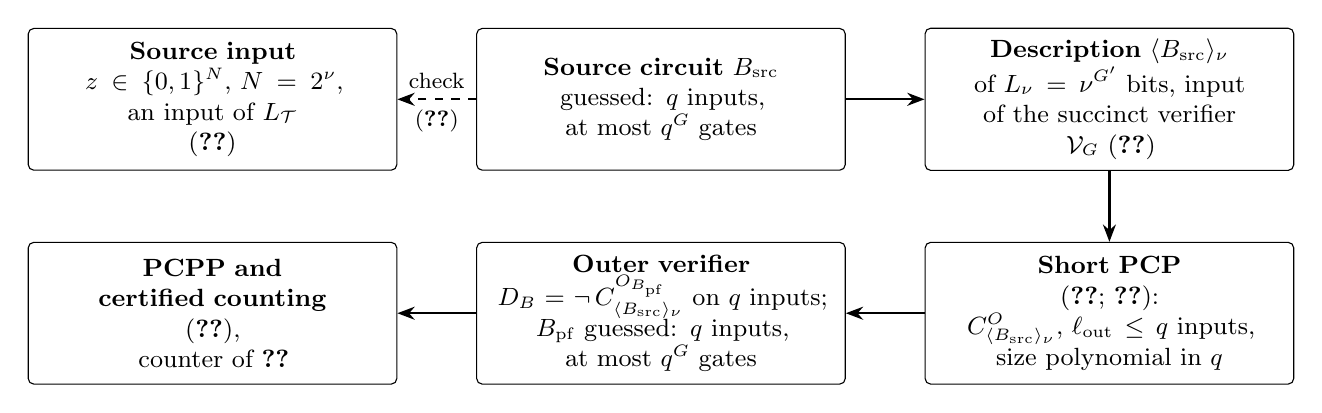
\begin{tikzpicture}[
  font=\small,
  box/.style={draw,rounded corners=2pt,align=center,inner sep=4pt,
              text width=44mm,minimum height=18mm},
  flow/.style={-{Stealth[length=2.2mm]},thick},
  lab/.style={font=\footnotesize,align=center},
  node distance=9mm and 10mm]
\node[box] (z) {\textbf{Source input}\\ \(z\in\{0,1\}^N\), \(N=2^\nu\),\\
  an input of \(L_{\Tclk}\)\\ (\cref{imp:ae-refuter})};
\node[box,right=of z] (src) {\textbf{Source circuit} \(B_{\rm src}\)\\
  guessed: \(q\) inputs,\\ at most \(q^G\) gates};
\node[box,right=of src] (desc) {\textbf{Description}
  \(\langle B_{\rm src}\rangle_\nu\)\\ of \(L_\nu=\nu^{G'}\) bits, input\\
  of the succinct verifier\\ \(\mathcal V_G\) (\cref{app:multitape})};
\node[box,below=of desc] (pcp) {\textbf{Short PCP}\\
  (\cref{imp:short-pcp}; \cref{app:short-pcp-proof}):\\
  \(C^O_{\langle B_{\rm src}\rangle_\nu}\), \(\ell_{\rm out}\le q\) inputs,\\
  size polynomial in \(q\)};
\node[box,left=of pcp] (D) {\textbf{Outer verifier}\\
  \(D_B=\neg\,C^{O_{B_{\rm pf}}}_{\langle B_{\rm src}\rangle_\nu}\)
  on \(q\) inputs;\\ \(B_{\rm pf}\) guessed: \(q\) inputs,\\ at most
  \(q^G\) gates};
\node[box,left=of D] (pcpp) {\textbf{PCPP and}\\
  \textbf{certified counting}\\
  (\cref{sec:gadget-transfer}),\\ counter of
  \cref{thm:pair-uniform}};
\draw[flow,dashed] (src) -- node[lab,above]{check} node[lab,below]{\eqref{eq:source-check}} (z);
\draw[flow] (src) -- (desc);
\draw[flow] (desc) -- (pcp);
\draw[flow] (pcp) -- (D);
\draw[flow] (D) -- (pcpp);
\end{tikzpicture}
\caption{The fixed weak machine of \cref{sec:gadget-machine}. The source input enters
only the deterministic source check. The short PCP sees only a
description of polynomially many bits in \(q=\Theta(\log N)\), so every
later object has size polynomial in~\(q\). At the refuter's rejected
yes-instance, the source input is hard for general circuits when no
source circuit exists (\textsc{NoSource}), and so is the first accepted
oracle when no small proof-oracle circuit computes it (\textsc{NoProof});
both are then amplified. Otherwise (\textsc{Tautology}) the honest weighted
local-proof table of the canonical pair selected in \cref{sec:gadget-extract}
is the hard function.}
\label{fig:outer-step}
\end{figure}

The constants of this subsection are chosen in the order $\epsilon$ (from
$d$ or $\rho$ and $\gamma$), $\eta_0$ (from \cref{thm:pair-uniform}), $d_0$,
$G$, $G'$, $C_{\rm clk}$, $A_{\rm pad}$, $d_G$, and finally the padding and
cap constants; the order-of-constants list at the end of
\cref{app:multitape} checks that no constant depends on one chosen after
it. Both theorems use one parameter template. For the fixed-error
theorem, choose a fixed $\epsilon=2^{-e_0}$, for a positive integer $e_0$, with
$\epsilon<\gamma/10$ and $d<\gamma/5-\epsilon$, and set
$\epsilon_q=\epsilon$. For the boundary theorem, set
\[
 \epsilon_q=2^{-\rho(2\lambda_q)}.
\]
In both cases put
\begin{equation}\label{eq:gadget-parameters}
 P_q=128/\epsilon_q,\qquad
 \omega_q=\epsilon_q/128,\qquad
 b(q)=\left\lfloor\eta_0\epsilon_q\mathcal A_3(q)\right\rfloor,
\end{equation}
where $\eta_0>0$ is a fixed rational smaller than $a_{1,1}/512$,
and $a_{1,1}$ is the constant in \cref{thm:pair-uniform} for
inverse-polynomial precision exponent and bit envelope both equal to
one. Think of $P_q$ as the number of addresses per gadget (the honest
table repeats each of its five entries about $P_q/5$ times), of
$\omega_q$ as the radius requested from the counter, and of $b(q)$ as the
native weight cap, an $\eta_0\epsilon_q$ fraction of the counter's pair
cap. The integer $P_q$ is a power of two. Eventually
$\omega_q\ge q^{-1}$, its representation has at most $q$ bits,
and $\epsilon_q<\gamma/10$. The weak machine checks these conditions
before guessing anything. Two circuits of weight at most $b(q)$
have total weight below $a_{1,1}\omega_q\mathcal A_3(q)$.
Check the exponent and representation-length bounds before expanding
any power of two; failed finite public guards cause immediate rejection.

We use the published short PCP, general-circuit amplifier, and
fixed-machine refuter from \cref{sec:imports}. There is a fixed
integer $h_{\rm sim}$ such that, for every fixed $A\ge1$ and all
sufficiently large $q$, every target circuit on at most $Aq$ inputs and
of weight at most $q^3$ has a general Boolean simulation of size
$q^{h_{\rm sim}}$. Normalize its bottom thresholds, evaluate their integer
linear forms, form the top sum, and look up the polynomial-length output
table. All integers have polynomial bit length, and the size is a fixed
polynomial in $q$ and the number of inputs, so one exponent serves every
fixed $A$. Choose a fixed integer $G$ with $G/b_{\rm amp}>h_{\rm sim}+1$,
using the exponent in \cref{imp:ae-amplification}, and let $a_G$ be its
arity constant for this $G$.

Take $\Tclk(N)=N^{C_{\rm clk}}$. The hierarchy language
$L_{\Tclk}$ of \cref{imp:ae-refuter} has a nondeterministic multitape
verifier $\mathcal D$ that halts within $O(\Tclk(N))$ steps on every input and witness (\cref{lem:multitape-refuter}), with no short-witness
restriction. Only source lengths $N=2^\nu$ are used
(\cref{sec:all-lengths}); the weak machine rejects every input whose
length is not a power of two.

The circuit of \cref{imp:short-pcp} grows with the length of its
explicit input, so the short PCP is not applied to the source input
itself. Instead the weak machine guesses a small general circuit for
the source input, checks it at every position, and applies the short
PCP to the description of that circuit.

For a general circuit $B$ with
$a\ge\nu$ inputs, let $\mathrm{tt}_N(B)\in\{0,1\}^N$ be the word whose
$i$th bit is $B(\mathrm{bin}_\nu(i)0^{a-\nu})$, where
$\mathrm{bin}_\nu(i)$ is the $\nu$-bit binary expansion of $i<N$. Fix a
self-delimiting binary description of general circuits that lists the
gates, so that a description of $n$ bits has at most $n$ gates, and
whose length is polynomial in the numbers of gates and inputs. Fix an integer
$G'\ge2$, depending only on $G$ and on this description format, such
that for all large $\nu$ every description of a circuit with at most
$q^G$ gates on $q$ inputs has fewer than $\nu^{G'}$ bits. Such a $G'$
exists: these descriptions have length at most a fixed polynomial in
$q=O(\nu)$ whose degree depends only on $G$ and the format, and any $G'$
above that degree works. Put
\[
 L_\nu=\nu^{G'},
\]
and, when the description of $B$ has at most $L_\nu$ bits, let
$\langle B\rangle_\nu\in\{0,1\}^{L_\nu}$ be that description followed by
zeros.

\Cref{lem:succinct-verifier} in \cref{app:multitape} gives one
deterministic multitape verifier $\mathcal V_G(u,y)$, a nondecreasing
time bound $T_G(n)\ge n$ within which $\mathcal V_G$ halts on every input
of length $n$ and every witness, and a constant $c_G$. They satisfy
$T_G(L_\nu)=c_G\Tclk(N)$, and, for every such $B$, some witness of length
$T_G(L_\nu)$ makes $\mathcal V_G$ accept $\langle B\rangle_\nu$ exactly
when $\mathrm{tt}_N(B)\in L_{\Tclk}$. The only size bound that
$\mathcal V_G$ places on $B$ is the length $L_\nu$, which depends on
$N$ and the fixed $G'$ alone; the weak machine enforces the bound $q^G$
separately. Only three properties of $L_\nu$ are used:
\begin{itemize}
\item it is a fixed polynomial in $\nu$;
\item it has degree at least two;
\item it eventually exceeds the description length of every circuit
with at most $q^G$ gates on $q$ inputs.
\end{itemize}
$L_\nu$ is fixed before $\mathcal V_G$, and these
properties hold whatever constants are chosen after it.

We apply \cref{imp:short-pcp} once, to $\mathcal V_G$ with the time bound
$T_G$, which is computable from the input length in polynomial time, as
that input requires (\cref{lem:succinct-verifier}(i)). On an input $\langle B\rangle_\nu$ it constructs, in time
$\poly(L_\nu,\log T_G(L_\nu))=\nu^{O_{G,C_{\rm clk}}(1)}$, an oracle circuit
$C^O_{\langle B\rangle_\nu}$ of size $\nu^{O_{G,C_{\rm clk}}(1)}$ with
$\ell_{\rm out}=\lgx\Tclk(N)+O(\log\log\Tclk(N))$ inputs. Pad it to the
exact native width
\[
 q(N)=\lceil\log_2\Tclk(N)\rceil+
 A_{\rm pad}\lceil\log_2(\log_2\Tclk(N)+2)\rceil+A_{\rm pad},
\]
by adding inputs that it ignores, for a sufficiently large fixed integer
$A_{\rm pad}$, chosen after $C_{\rm clk}$ as at the end of
\cref{app:multitape} so that $\ell_{\rm out}\le q(N)$. Then
$q=\Theta(\log N)$ and $2^q/\Tclk(N)=q^{O(1)}$.

On a source input $z\in\{0,1\}^N$, the weak machine first rejects
unless $N=2^\nu$ is a power of two. It computes a
fixed polynomial envelope for all its guesses and rejects if it
exceeds $\lfloor N/16\rfloor$. It also checks the precision guards
above and $\gamma/L_\nu<\epsilon_q$, and it rejects unless the
description of the source circuit $B_{\rm src}$ guessed below has at
most $L_\nu$ bits. By the choice of $G'$, once $\nu$ is large every
general circuit with $q$ inputs and at most $q^G$ gates has such a
description, so the last guard rejects at only finitely many lengths.
Since $q=\Theta(\nu)$ and
$G'\ge2$, $\gamma/L_\nu=O(q^{-2})$, while $\epsilon_q\ge128/q$
eventually under both schedules; so these guards, too, fail at only
finitely many lengths.

The machine guesses a general circuit $B_{\rm src}$ with $q$ inputs and
at most $q^G$ gates, the \emph{source circuit}, rejecting malformed
descriptions. It then checks deterministically that
\begin{equation}\label{eq:source-check}
 B_{\rm src}\bigl(\mathrm{bin}_\nu(i)0^{q-\nu}\bigr)=z_i
 \qquad\text{for every }i<N,
\end{equation}
that is, $\mathrm{tt}_N(B_{\rm src})=z$, and rejects otherwise. It
constructs $C^O_{\langle B_{\rm src}\rangle_\nu}$, whose number
$\ell_{\rm out}$ of inputs may depend on $B_{\rm src}$, and guesses a
general circuit $B_{\rm pf}$ with $q$ inputs and at most $q^G$ gates,
the outer proof oracle, again rejecting malformed descriptions. It
answers an oracle query $a\in\{0,1\}^{\ell_{\rm out}}$ by
\[
 O_{B_{\rm pf}}(a)=B_{\rm pf}\bigl(a0^{q-\ell_{\rm out}}\bigr),
\]
the same zero padding as in \eqref{eq:source-check}. Write
$B=(B_{\rm src},B_{\rm pf})$. Substituting $O_{B_{\rm pf}}$ for every
oracle gate and negating the output gives the outer verifier
\[
 D_B(x)=\neg\,C^{O_{B_{\rm pf}}}_{\langle B_{\rm src}\rangle_\nu}
 (x_1,\ldots,x_{\ell_{\rm out}}),\qquad x\in\{0,1\}^q,
\]
which ignores its last $q-\ell_{\rm out}$ inputs. The negation turns
the convention of \cref{imp:short-pcp} into the usual one: $D_B(x)=1$
means that the outer verifier accepts the random string $x$. Since
$L_\nu\le q^{G'}$, $D_B$ is a circuit of size $q^{O_{G,C_{\rm clk}}(1)}$ on $q$
inputs. The exponent depends on $C_{\rm clk}$ as well, through
$\mathcal V_G$; this is harmless, because the constants that depend on
it, beginning with the exponent $d_G$ below, are chosen after
$C_{\rm clk}$ (\cref{app:multitape}). Apply \cref{imp:three-pcpp}. Choose a fixed $d_G$ bounding
all resulting clause counts and repeat the whole clause list to
exactly
\[
 M=2^{\lceil d_G\log_2(q+2)\rceil}
\]
clauses. If the list is longer than $M$, which happens at only
finitely many lengths, the machine rejects. The original length divides
this number. This fixes the eventual table arity independently of the
guessed pair.

For each resulting three-literal clause introduce a fresh helper name,
disjoint from all original auxiliary and systematic names. The
machine guesses one normalized target circuit of weight at most
$b(q)$ for each distinct auxiliary name, including every fresh
helper. All appearances of one name use this same circuit.
Systematic coordinates are supplied exactly as the prescribed
parities. Reject malformed or oversized descriptions. The weight test $W\le b(q)$ is the
integer comparison $W^4\lambda_q^{21}\mu_q^{28}\le(\eta_0\epsilon_q)^4q^{12}$. Only existence
of normalized integer descriptions is required; an efficient
normalization algorithm is not assumed.

Finally guess the polynomial-length witness prefixes for the nonexact
counter calls in \cref{eq:gadget-pair-identity}, each requesting
radius $\omega_q$, form the certified upper
estimate $U$, and accept exactly when
\begin{equation}\label{eq:gadget-acceptance}
 U<\gamma-\epsilon_q.
\end{equation}

On a hierarchy no-instance $z$, consider a branch whose source circuit
passes the check \eqref{eq:source-check}; every other branch rejects.
Then $\mathrm{tt}_N(B_{\rm src})=z\notin L_{\Tclk}$, so $\mathcal V_G$
rejects $\langle B_{\rm src}\rangle_\nu$ with every witness, and by
\cref{imp:short-pcp} the circuit
$C^{O_{B_{\rm pf}}}_{\langle B_{\rm src}\rangle_\nu}$ is satisfied by at
least a $1-1/L_\nu$ fraction of its inputs. Hence $D_B(x)=1$
on at most a $1/L_\nu$ fraction of inputs. On every remaining
input, \cref{imp:three-pcpp} forces at least a $\gamma$ fraction
of false original clauses, each contributing penalty at least one.
All other penalties are nonnegative. Consequently every Boolean
guess satisfies
\[
 \mathbb E Q\ge\gamma(1-1/L_\nu)>\gamma-\epsilon_q.
\]
Every witness has $U\ge\mathbb E Q$, so every branch rejects.

All guesses have a fixed polynomial bound in $q$ and hence are
$o(N)$; the initial guard enforces the stated limit at every length.
Evaluating a circuit with at most $q^G$ gates takes $q^{O(G)}$ steps,
so the check \eqref{eq:source-check} takes $Nq^{O(G)}\le N^{d_0}$ steps
for $d_0=2$ and all large $N$. This exponent depends on no PCP
construction. Constructing $C^O_{\langle B_{\rm src}\rangle_\nu}$ and
$D_B$ takes $q^{O_{G,C_{\rm clk}}(1)}=N^{o(1)}$ steps by \cref{imp:short-pcp}. Choose an integer
$C_{\rm clk}>d_0+2$. The polynomially many
pair calls and their deterministic multiword arithmetic overhead
take
\[
 2^q q^{O(1)-\mu_q}=o(\Tclk(N)).
\]
Polynomial-bit arithmetic is expanded into operations on
$O(\log T)$-bit words; no new nondeterministic bits are needed.
The refuter therefore applies to this one fixed weak machine. At
every sufficiently large source length it returns a hierarchy
yes-instance that the weak machine rejects.

\subsection{Extracting a hard table}
\label{sec:gadget-extract}

Fix such a rejected yes-instance $z\in\{0,1\}^N$, with $N=2^\nu$. The
two cases below, the
SAT-checked canonical choices, and the clause-indexed proof table
follow Chen--Lyu--Williams~\cite[Sections~6.2.4--6.2.5]{CLW20}.
Their proof of~\cite[Lemma~6.5]{CLW20} averages cofactors into
real-valued proofs; we instead select one
Boolean cofactor per name and weight the list positions. Call a general
circuit with $q$ inputs and at most $q^G$ gates a \emph{source circuit
for $z$} if it satisfies \eqref{eq:source-check}. Descriptions are
ordered lexicographically, and ``first'' refers to this order. The
canonical choices are made in three steps, which yield the three cases
named in \cref{sec:overview}.
\begin{enumerate}[label=(\roman*)]
\item (\textsc{NoSource}) If $z$ has no source circuit, let $X_z:\{0,1\}^q\to\{0,1\}$ map
$u$ to $z_i$, where $\mathrm{bin}_\nu(i)$ is the first $\nu$ coordinates
of $u$. A general circuit of at most $q^G$ gates computing $X_z$ would
be a source circuit for $z$. Hence $X_z$ has general circuit complexity
greater than $q^G$.
\item Otherwise let $B^*_{\rm src}$ be the first source circuit for $z$.
Then $\mathrm{tt}_N(B^*_{\rm src})=z\in L_{\Tclk}$, so some witness of
length $T_G(L_\nu)$ makes $\mathcal V_G$ accept
$\langle B^*_{\rm src}\rangle_\nu$, and \cref{imp:short-pcp} provides an
oracle on $\ell_{\rm out}$ inputs that makes
$C^O_{\langle B^*_{\rm src}\rangle_\nu}$ unsatisfiable, that is,
accepted on every random string. Let $O^*$ be the first such oracle,
viewed as a truth table, and let $\widehat O^*(av)=O^*(a)$ for
$a\in\{0,1\}^{\ell_{\rm out}}$ and $v\in\{0,1\}^{q-\ell_{\rm out}}$.
\item (\textsc{NoProof}) If no general circuit $B_{\rm pf}$ with $q$ inputs and at most
$q^G$ gates satisfies $O_{B_{\rm pf}}=O^*$, then $\widehat O^*$ has
general circuit complexity greater than $q^G$, since a circuit computing
it would satisfy that equation.
\end{enumerate}
Cases (\textsc{NoSource}) and (\textsc{NoProof}) are treated together. In each of them
we obtain a function on $q$ inputs with general circuit complexity
greater than $q^G$. By
\cref{imp:ae-amplification} and the choice of $G$, the
amplified function, on at most $a_Gq$ inputs, has agreement $1/2+o(1)$
against every target circuit considered here. This is eventually below
$1-\gamma/5+\epsilon_q$.

Otherwise, in case (\textsc{Tautology}), let $B^*_{\rm pf}$ be the first
general circuit with $q$ inputs and at most $q^G$ gates such that
$O_{B^*_{\rm pf}}=O^*$, and put
$B=(B^*_{\rm src},B^*_{\rm pf})$. Then $D_B$ is a tautology, because
$C^{O^*}_{\langle B^*_{\rm src}\rangle_\nu}$ is unsatisfiable, and its
source circuit passes the check \eqref{eq:source-check}, so the weak
machine can guess $B$. This canonical choice suffices: the argument
below uses only that $B$ is a pair whose source circuit passes the
check, that $D_B$ is a tautology, and that the weak machine rejected $z$
on every branch, including those that guess $B$. The efficient honest proof from
\cref{imp:three-pcpp} defines Boolean coordinate functions $\Pi_X(x)$
that make every three-literal clause true. For each fresh helper, define its
honest function to be the AND of that clause's three honest literal
values. For gadget $a$, form the five-entry list of underlying
coordinate names
\[
 (X_{a,1},X_{a,2},X_{a,3},Y_a,Y_a).
\]
The first three entries are unsigned names: the clause's literal
signs remain in the verifier, not in the table definition. Fill
$P_q$ address positions by cycling through this list, and define
the target table to return the corresponding honest coordinate.
Its exact arity is
\begin{equation}\label{eq:gadget-table-arity}
 q_0(q)=q+\log_2M+\log_2P_q=q+O(\log q).
\end{equation}

Suppose a target circuit $C$ of weight at most $b(q)$ approximates
this table with error $\delta$. For each auxiliary name choose,
among the addresses whose list entry is that name, one minimizing
the error of the cofactor
$C(x,\text{address})$ against that name's honest function. Use that
one cofactor at every occurrence of the name. These are literal
restrictions of $C$, with unchanged top weight. Systematics remain
exact. The chosen integer descriptions can be guessed by the weak
machine.

Let $t_q=\lfloor P_q/5\rfloor$. If a name has total stability weight
$I_X$ across the five-entry lists (one per literal occurrence, two
for a helper, as in \cref{lem:gadget-stability}), it appears in at
least $t_qI_X$
table positions. The minimum error is at most its occurrence-average
error. Write $e_X$ for the chosen cofactor's error and
$\mathrm{err}(a,j)$ for the error of $C$ at address $(a,j)$, so that
$\delta$ is the average of $\mathrm{err}$ over all $MP_q$ addresses.
Applying \cref{lem:gadget-stability} pointwise and summing over names,
\[
 \mathbb E Q\le\frac1M\sum_XI_Xe_X
 \le\frac1{Mt_q}\sum_{a,j}\mathrm{err}(a,j),
\]
which gives
\begin{equation}\label{eq:gadget-table-error}
 \mathbb E Q\le\frac{P_q}{\lfloor P_q/5\rfloor}\delta.
\end{equation}
This argument also covers repeated names within one clause and
different literal signs on the same name. Each fresh helper has one
common guessed value despite appearing twice in its five-entry list.

Since $P_q=128/\epsilon_q$ and $0<\epsilon_q<1$,
\[
 \frac{P_q}{\lfloor P_q/5\rfloor}\le5+\epsilon_q.
\]
If $\delta\le\gamma/5-\epsilon_q$, a useful counting witness yields
\begin{align*}
 U&\le(5+\epsilon_q)(\gamma/5-\epsilon_q)+10\omega_q\\
  &\le\gamma-4\epsilon_q+10\epsilon_q/128
   <\gamma-\epsilon_q.
\end{align*}
This would be an accepting branch on the rejected source input.
We conclude that the table has agreement strictly below
$1-\gamma/5+\epsilon_q$ at native weight $b(q)$.

\subsection{Every sufficiently large length and uniform recovery}
\label{sec:all-lengths}

Choose a fixed integer $K_{\rm amp}\ge a_G$ large enough
to accommodate the general amplifier, and pad the function in either
case to exactly $m(q)=K_{\rm amp}q_0(q)$ inputs, ignoring a suffix.
Use source lengths $N_\nu=2^\nu$. The native widths $q(N_\nu)$ have
bounded additive jumps. For a final length $n$, choose the largest $\nu$
with $m(q(N_\nu))\le n/2$. When none exists, set the slice to zero.

The boundary schedule can have jumps, so bounded additive gaps in
$m(q)$ should not be assumed. Instead, the next native width is
$q+O(1)$ and, by \cref{eq:gadget-table-arity}, its entire core has
length $K_{\rm amp}q+O(\log q)$. Maximality consequently gives
\[
 q\le n\le B_{\rm len}q
\]
eventually, for a fixed constant $B_{\rm len}$. Monotonicity of $\rho$
makes the core schedule monotone, so this selection is effective.
If a circuit approximates the padded function, averaging over the
ignored suffix gives a restriction with at least the same agreement
and no larger top weight.

For the fixed-error schedule, $b(q)=\lfloor\eta_0\epsilon
\mathcal A_3(q)\rfloor$ and
$\mathcal A_3(n)\le B_{\rm len}^3\mathcal A_3(q)$. Choosing
$K_d>2B_{\rm len}^3/(\eta_0\epsilon)$ handles the floor and the native cap.
Since $d<\gamma/5-\epsilon$, this proves
\cref{thm:main}.

For the boundary schedule, $\lambda_n\le2\lambda_q$ eventually,
and hence
\[
 \epsilon_q\le2^{-\rho(\lambda_n)},\qquad
 2^{-\rho(2\lambda_n)}\mathcal A_3(n)
 \le B_{\rm len}^3\,2^{-\rho(2\lambda_q)}\mathcal A_3(q).
\]
Choose $K>2B_{\rm len}^3/\eta_0$ to handle the cap and its floor. These
inequalities prove the claimed advantage bound. Moreover
$2^{\rho(2\lambda_n)}=n^{o(1)}$, so the same cap eventually
contains every fixed $An^{3-\alpha}$. The error bound tends
to $\gamma/5$, proving the common-language quantifiers in
\cref{thm:gadget-boundary}.

For completeness, all canonical choices are recoverable in $\ENP$.
The fixed-machine refuter runs in $\operatorname{poly}(\Tclk(N_\nu))
=2^{O(q)}$ time with SAT access. The choices of
\cref{sec:gadget-transfer} are recovered in three stages, by prefix
self-reduction on SAT formulas of size $2^{O(q)}$. First, a formula over
the description of $B_{\rm src}$ with the $N$ constraints
\eqref{eq:source-check}, of size $Nq^{O(G)}$, finds the first source
circuit $B^*_{\rm src}$, or shows that there is none, in which case the
table is $X_z$. Second, the algorithm of \cref{imp:short-pcp} is run
deterministically on $\langle B^*_{\rm src}\rangle_\nu$, in
$q^{O_{G,C_{\rm clk}}(1)}$ time; a formula with one variable per oracle address and the
constraints $C^O_{\langle B^*_{\rm src}\rangle_\nu}(R)=0$ for all
$2^{\ell_{\rm out}}$ inputs $R$, of size
$2^{2\ell_{\rm out}}q^{O_{G,C_{\rm clk}}(1)}=2^{O(q)}$ (each oracle gate
becomes a selector over the $2^{\ell_{\rm out}}$ oracle variables),
finds the first oracle $O^*$. The algorithm of
\cref{thm:short-pcp-ours} is non-adaptive: its queries depend on the
random string alone (\cref{rem:short-pcp-nonadaptive}), so for it each oracle gate reads a fixed
variable once $R$ is fixed, and the size is also
$2^{\ell_{\rm out}}q^{O_{G,C_{\rm clk}}(1)}$. Third, a formula over the description of
$B_{\rm pf}$ with the $2^{\ell_{\rm out}}$ constraints
$B_{\rm pf}(a0^{q-\ell_{\rm out}})=O^*(a)$, of size
$2^{\ell_{\rm out}}q^{O(G)}$, finds the first $B^*_{\rm pf}$, or shows
that there is none, in which case the table is $\widehat O^*$. No formula
contains the algorithm of \cref{imp:short-pcp}. Run the general amplifier
on $X_z$ or $\widehat O^*$. If no oracle $O^*$ exists at an exceptional
initial source length, the second stage detects that case and the slice
is set to zero. In the
small-oracle branch, the honest PCPP proof and each AND helper are
computable in polynomial time once the pair is known. Every new
schedule is computable in polynomial time in $q$. Since $q=O(n)$,
the final functions belong to $\ENP$.

\begin{proof}[Proof of \cref{cor:main-boundary}]
Take \(\rho(u)=\ceil{\lgx(u+2)}\) in
\cref{thm:gadget-boundary}. This is a polynomial-time computable,
nondecreasing, unbounded sublinear integer schedule. If \(K\)
is its cap constant, then
\(2^{\rho(2\lambda_n)}\le4\lambda_n+4\le8\lambda_n\).
Taking \(C_0\ge8K\) places the corollary's cap within that theorem's
cap, including its floor. Also
\(2^{-\rho(\lambda_n)}\le1/(\lambda_n+2)<1/\lambda_n\).
Use the theorem's fixed language as \(F\).
\end{proof}

\section{What remains open at the cubic scale}\label{sec:scope}

The main theorem combines an exponent improvement with
almost-everywhere constant-error hardness. Three extensions remain
distinct challenges.

\paragraph{Vanishing correlation for arbitrary symmetric tops.}
The weighted local-proof table uses only single and pair means. In the
signed-sum XOR reconstruction of Chen--Lyu--Williams~\cite{CLW20},
guessed proof coordinates can instead be arbitrary real signed sums
of circuit outputs. Certifying that such a coordinate \(S\) behaves
like a Boolean value uses the nonnegative test \(S^2(1-S)^2\), whose
expectation requires products of four outputs. The pair counter does
not supply these probabilities at the near-cubic cap. A method for
counting them, or a transfer avoiding that requirement, would address
the missing step. Applying an XOR lemma to \cref{thm:main} alone does
not establish the desired circuit lower bound.

\paragraph{Beyond the cubic exponent.}
The two-score window is close, up to logarithms, to the dimension
bound for reconstructing unrestricted histograms from these modular
data (\cref{rem:rank}). Improving this particular window alone cannot
supply another polynomial gain. One could seek further localization,
exploit restrictions on histograms arising from threshold circuits,
or use different measurements. The scalar counter's near-\(n^{7/2}\)
capacity is larger, but a lower-bound transfer must pay for all joint
probabilities it needs.

\paragraph{Broader circuit classes and more explicit hard functions.}
Unbounded unequal top weights in \(\THR\circ\THR\) are not controlled
by our gate budget. Extending the exponent to that model remains
open. So does obtaining the same gate exponent with a hard function
in \(\mathrm P\), rather than \(\ENP\). Neither extension follows
from the restriction estimate or the formal proof companion.

\appendix
% Name appendix sections "Appendix" in cross-references.
\makeatletter
\@ifpackageloaded{cleveref}{\crefalias{section}{appendix}%
  \crefalias{subsection}{subappendix}%
  \crefalias{subsubsection}{subsubappendix}}{}
\makeatother
\section{Proofs of supporting lemmas with explicit constants}\label{app:standard}

The three proofs below give the explicit constants and encodings
used by the counting algorithm. Attributions appear with each statement.


\subsection{Live gates}\label{app:live}
\begin{proof}[Proof of \cref{lem:live}]
A threshold gate is unate, so the chain-counting argument in the
proof of \cite[Lemma~A.3.1]{CTW26}, which combines their (14) and (15),
bounds the fraction of restrictions leaving \(g\) live by
\(k\binom{n-k}{\floor{(n-k)/2}}2^{-(n-k)}\). For the second inequality
put \(M=n-k\). If \(M=2r\), the quantities
\((\binom{2r}r4^{-r})^2(2r+1)\) start at one and decrease, because
their successive ratio is \((2r+1)(2r+3)/(2r+2)^2<1\).
The odd case \(M=2r+1\) follows from
\(\binom{2r+1}r2^{-2r-1}=\binom{2r}r4^{-r}(2r+1)/(2r+2)
\le\sqrt{2r+1}/(2r+2)<1/\sqrt{2r+2}\).
Finally, sum the probability estimate over signed unit copies, fix
\(I\) by averaging, and apply Markov's inequality over \(y\).
\end{proof}

\subsection{Totient sums and the two-score window}\label{app:window-size}
\begin{proof}[Proof of \cref{lem:window-size}]
These are standard totient-summation calculations; see
Apostol~\cite[Chapters~2--3 and~11]{Apostol76} for the M\"obius
identities, arithmetic averages, and Euler products.
Write \(\mu\) for the M\"obius function. Since
\(m\varphi(m)=\sum_{d\mid m}\mu(d)m^2/d\),
\[
 S(q)=\sum_{d\le q}\mu(d)d\sum_{e\le q/d}e^2.
\]
The sum-of-squares formula gives
\(\abs{\sum_{e\le y}e^2-y^3/3}\le y^2\) for \(y\ge1\).
Therefore
\[
 S(q)\ge\frac{q^3}{3}\sum_{d\le q}\frac{\mu(d)}{d^2}
          -q^2\sum_{d\le q}\frac1d.
\]
Use \(\sum_{d\ge1}\mu(d)/d^2=6/\pi^2\), a tail of magnitude at most
\(1/q\), and \(\sum_{d\le q}1/d\le1+\ln q\).
For \(L=\floor{cD'^{3/4}}\), the associated \(q\) is
\((1/c+o(1))D'^{1/4}\). Thus \(S(q)\ge L\) eventually whenever
\(c^4<2/\pi^2\); this includes \(c=3/5\).
Conversely \(S(q)\le\sum_{m\le q}m^2=O(q^3)\), and
\(q\le(D'-1)/(L-1)\), so every admissible \(L\) is
\(O(D'^{3/4})\).
\end{proof}


\subsection{Disjoint exact-threshold decomposition}\label{app:exact}
\begin{proof}[Proof of \cref{lem:exact}]
Complement negative-weight inputs, obtaining
\(g=\ind[\sum_i\abs{a_i}\widehat z_i\ge t']\).
If \(t'\le0\) or \(t'>\sum_i\abs{a_i}\), use a constant exact test.
Otherwise \(0<t'\le\sum_i\abs{a_i}<2^{B_b}\). Define
\[
 d_j=\floor{t'/2^j}-\sum_i\floor{\abs{a_i}/2^j}\widehat z_i,
 \qquad 0\le j\le B_b.
\]
Then \(d_{B_b}=0\), \(g=\ind[d_0\le0]\), and
\[
 d_j=2d_{j+1}+r_j,\qquad -m\le r_j\le1.
\]
Here \(r_j=\tau_j-\sum_i\delta_{ij}\widehat z_i\), where \(\tau_j\) and
\(\delta_{ij}\) are the \(j\)th binary digits of \(t'\) and \(\abs{a_i}\),
because \(\floor{c/2^j}=2\floor{c/2^{j+1}}+c_j\) for every integer
\(c\ge0\) with \(j\)th binary digit \(c_j\). Thus \(r_j\) is an affine
form with coefficient magnitudes at most one.
If \(d_{j+1}<0\), then \(d_j\le-1\): negativity persists toward
smaller indices. Thus
\[
 \ind[d_0\le0]
 =\ind[d_0=0]+\sum_{j<B_b}\ind[d_{j+1}\ge0>d_j]
\]
is a disjoint sum. At a crossing, the pair
\((a,b)=(d_{j+1},d_j)\) satisfies
\(0\le a\le\floor{(m-1)/2}\) and \(-m\le b\le-1\).
There are at most \(m\ceil{m/2}\) such pairs per level.

Discard a pair if \(b-2a\notin[-m,1]\). For each remaining pair, use
the single exact test
\[
 (m+2)(d_{j+1}-a)+\bigl(r_j-(b-2a)\bigr)=0.
\]
The second term has magnitude at most \(m+1\). Reducing the equality
modulo \(m+2\) forces this term to be zero, then forces
\(d_{j+1}=a\) and \(d_j=b\). All displayed coefficients have the
claimed bit length. The tests are disjoint because the crossing
level and its pair are unique.
\end{proof}


\section{Source mapping for the published inputs}\label{app:sources}

The principal published inputs are listed below with their source
locations and adaptations; supporting references appear at their points
of use. Each listed statement was checked against a copy of its source. \emph{Verbatim}
means the statement is used as the source states it; \emph{adapted}
records what changed.

\begin{center}\footnotesize
\begin{tabularx}{\textwidth}{@{}>{\raggedright\arraybackslash}p{.21\textwidth}
 >{\raggedright\arraybackslash}p{.30\textwidth}>{\raggedright\arraybackslash}X@{}}
\toprule
Statement here & Source location & Use and adaptation\\
\midrule
\Cref{imp:batch}, rectangular product &
\cite[Corollary~4.4 = Corollary~C.2, and Appendix~C]{WilACC14}; \cite{Cop82} &
Adapted: the dimensions \(N^{0.1}\) are read as \(\ceil{N^{0.1}}\), and the uniform multitape clause is Williams' Appendix~C. The same import is used in \cite[Appendix~B]{NagCubic}.\\
\Cref{lem:signed-boolean-product,lem:signed-printer}, signed printing &
\cite[Appendix~B]{NagCubic}; \cite{Mat91} &
Proved here: binary slicing and Matou\v{s}ek's bucketing reduce signed exact-threshold printing to \cref{imp:batch}.\\
\Cref{imp:short-pcp}, short PCP &
\cite[Section~5, proof of Theorem~1.4, and footnote~5]{MW20}, credited there to \cite[Theorem~1.1]{BV14} &
Adapted: the implicit hypothesis that \(T(n)\) is computable in \(\poly(n,\log T(n))\) time is stated; applied once, to the succinct verifier of \cref{lem:succinct-verifier}. Proved for multitape verifiers in \cref{thm:short-pcp-ours}; \cref{cor:short-pcp-clock} and its following interface paragraph give the clock-as-data and small-input clauses. The printed \cite[Theorem~1.1]{BV14} and its restatement \cite[Lemma~3.10]{CLW20} are not used (\cref{rem:bv14-printed}).\\
\Cref{thm:short-pcp-ours}, the short PCP for multitape verifiers &
\cite[Theorem~11.1 with Equation~(6) of Theorem~11.3]{BCGT13}; \cite[Corollary~3.2]{Sho88}, as used in \cite[Algorithm~17]{BCGT13}; the construction of \cite[Definitions~4.15, 7.1 and~8.4, Constructions~8.3 and~8.5, Remark~11.2, Lemmas~12.23 and C.2--C.8, recursions~(27)--(28) of Section~C.8]{BCGT13}; \cite[Lemma~4.7]{BV14} &
Adapted: each proximity sub-verifier runs once on a shared random string, and soundness is amplified with a small-bias set (\cref{lem:small-bias,lem:patch-r}, proved here) instead of naive repetition. The random-access simulation (\cref{lem:tm-ram}), the reduction to an affine constraint instance (\cref{thm:trace,thm:embedding,lem:acsp-degree,lem:generator}) and the soundness of the single-run verifier are proved here. The randomness and proof-length bounds at the parameter tuple used are proved here (\cref{lem:rs-recursion}); the general bound of \cite[Lemma~C.1]{BCGT13} is not used (\cref{rem:bcgt-c1}).\\
\Cref{imp:ae-refuter}, fixed-machine refuter &
\cite[Theorem~1.13 and Section~4.1]{CLW20}, formal version Theorem~4.6; \cite{FS16}; \cite[Lemma~3 and Condition~2]{SFM78}; \cite{BGW70} &
Derived: \cref{lem:multitape-refuter,cor:framed-refuter} use accepting-time universal simulation and faithful prefix verification to cover the full clock range, including linear clocks. The framed weak machine retains exactly \(\floor{N/16}\) witness bits; framing and simulation guesses belong to the hierarchy verifier.\\
\Cref{imp:ae-amplification}, amplification &
\cite[Lemma~3.9]{CLW20}; the reconstruction theorem \cite[Theorem~29]{STV01}, with the constructions and arguments of \cite[Theorem~24 and Lemmas~25, 27 and~28]{STV01} &
Derived: used at \(S(q)=q^G\), with absolute \(b_{\rm amp}\) and an arity factor depending on \(G\). The full-range argument below supplies the Lean formulation for every time-constructible \(S\), including every-length correctness and unconditional eventual runtime. Theorem~29 is the only premise taken from \cite{STV01}; the companion proves the binary code, the circuit reconstruction and the uniform construction from it.\\
\Cref{imp:three-pcpp}, three-query PCPP &
\cite[Lemma~22, at soundness \(1/2\), and Lemma~26]{CW19}; \cite{BGHSV06} &
Derived: the clause conversion of \cite[Appendix~A]{CW19}, which proves \cite[Lemma~24]{CW19}, is a proved step; only the encoder of \cite[Lemma~26]{CW19} is used. The stronger three-block code of \cite[Lemma~27]{CW19} is proved separately in the companion and is not needed. The uniform trimming and code argument below supplies polynomial proof length, the proximity-boundary convention, efficient honest proofs, and parity supports. The pointwise form checks systematic words instead of decoding, pads with tautologies to a power of two, and takes a smaller rational \(\gamma\).\\
\bottomrule
\end{tabularx}
\end{center}

\begin{center}\footnotesize
\begin{tabularx}{\textwidth}{@{}>{\raggedright\arraybackslash}p{.21\textwidth}
 >{\raggedright\arraybackslash}p{.30\textwidth}>{\raggedright\arraybackslash}X@{}}
\toprule
Statement here & Source location & Use and adaptation\\
\midrule
\Cref{lem:integer}, integer weights &
\cite[Lemma~3.2]{CTW26}; the classical fact is \cite{MTT61}; sharper bound in \cite[Section~3]{Has94} &
Verbatim.\\
\Cref{lem:live}, live gates &
\cite[Lemma~4.1; Lemma~A.3.1, (14)--(15)]{CTW26}; \cite{KW16,Lub66} &
Adapted: the explicit bound \(k/\sqrt{n-k+1}\) and the Markov step are added.\\
\Cref{lem:bernstein} &
\cite[Theorem~2.8.4, first edition]{Vershynin18}, with \(K=1\) &
Specialized to \(K=1\) and an upper bound \(V\) on the sum of the variances.\\
\Cref{lem:exact}, disjoint exact thresholds &
\cite[Theorem~7]{HP10}; \cite[Proposition~18(2), Appendix~B, Lemmas~48--49]{CW19} &
Own variant with explicit bit lengths, proved in \cref{app:exact}.\\
Packing \eqref{eq:pack} &
\cite[Proposition~18(5)]{CW19} &
Adapted: the source states the containment AND\(\circ\)ETHR\(\subseteq\)ETHR; the explicit packing formula is proved here.\\
\Cref{lem:amp}, modulus amplification &
\cite[Section~2.3]{BT94}; \cite{Tod91,Yao90}; used in \cite{WilACC14} &
Verbatim; the short proof is included.\\
\Cref{lem:two-window}, two-score window &
\cite[Theorem~1 and its divisibility lemma]{HT01} &
Adapted: modular reconstruction over \(\Q\) using all short primitive directions, with the explicit box-size bound in \cref{lem:window-size}.\\
\Cref{lem:primes}, prime count &
Prime number theorem \cite[Chapters~4 and~13]{Apostol76}; \cite{Erdos32} &
Derived: the prime number theorem gives the dyadic prime count; summation and \cref{lem:window-size} give the displayed window estimates.\\
Gadget and \cref{lem:gadget-stability} &
\cite{GJS76}, in the form of \cite[Lemma~47]{CW19}; the aggregate score is used in \cite[Lemma~25]{CW19} &
Adapted: the weighted stability bound is new.\\
Extraction and canonical recovery &
\cite[Sections~6.2.4--6.2.5 and Lemma~6.5]{CLW20} &
Adapted: one Boolean cofactor is selected per name instead of averaging cofactors.\\
\bottomrule
\end{tabularx}
\end{center}

\paragraph{Full-range amplification interface.}
We justify the formulation of \cite[Lemma~3.9]{CLW20} used by the
companion, for every time-constructible \(S:\mathbb N\to\mathbb N\).
Here circuit size counts all DAG nodes, including input and constant
nodes. Following the construction of \cite[Lemmas~25 and~28]{STV01}
and the circuit argument of its Theorem~24, the polynomial
reconstruction theorem \cite[Theorem~29]{STV01} gives absolute constants
\(A\ge1\) and an integer \(a\ge1\) with the following consequence. An
\(s'\)-node circuit agreeing with the encoded function on more than
a \(1/2+\delta\) fraction yields an exact circuit for the original
\(n\)-input function with at most
\(A(n/\delta)^a s'+n+2\) nodes. The polynomial reconstruction
overhead includes fixing the decoder's randomness and conversion
to our fan-in-two basis; the last term allows input and constant
nodes. Choose an integer \(c>2a+2\), once and before \(S\).

Every \(n\)-input function has a circuit with fewer than
\(U(n)=2^{n+3}\) nodes. Indeed Shannon expansion combines two
\((n-1)\)-input circuits as
\((x\wedge f_1)\vee(\neg x\wedge f_0)\), adding at most five nodes.
Thus \(B(0)=1\) and \(B(n)\le2B(n-1)+5\) give
\(B(n)\le6\cdot2^n-5<U(n)\).
For all sufficiently large \(n\), construct the output as follows.
If \(S(n)=0\), use a constant function: the target size is zero and
no circuit has zero nodes. If \(1\le S(n)\le n^c\), use parity on
\(n+1\) bits. A circuit with at most \(S(n)^{1/c}\le n\) nodes
omits an input, so pairing assignments that differ only in that
input gives agreement exactly \(1/2<1/2+S(n)^{-1/c}\).
If \(S(n)\ge U(n)\), use a constant function, since no input
function satisfies the hardness premise.

In the remaining regime \(n^c<S=S(n)<U(n)\), put
\(\epsilon=S^{-1/c}\). Compute the least integer \(k\) such that
\(2^{ck}\ge S\), and use the dyadic accuracy
\(\delta=2^{-k-2}\); then
\(\epsilon/8<\delta\le\epsilon/4\).
All parameter choices use integer arithmetic. Apply the binary
encoder of \cite[Lemma~28]{STV01} to the truth table.
A circuit of size at most \(S^{1/c}\) with agreement at least
\(1/2+\epsilon\) would have agreement strictly greater than
\(1/2+\delta\). After increasing the absolute constant \(A\) to
absorb \(8^a\), reconstruction gives size at most
\[
 A n^a S^{(a+1)/c}+n+2<S.
\]
The strict inequality holds uniformly in this regime from a fixed
onset: dividing by \(S>n^c\) bounds the left side by
\[
 \frac{A}{n^{\,c-2a-1}}+\frac{n+2}{n^c}<1.
\]
This contradicts the premise and proves the required strict
agreement bound.

For clarity about the truth-table layout, in the construction of
\cite[Lemmas~25 and~28]{STV01} choose a binary extension field,
rounding its size up to the required scale, and round the number
of polynomial variables up. The evaluation domain is then
\(\mathbb F^m\); concatenation with a Hadamard block indexes the
binary codeword by a product of binary cubes. Its length is a
power of two, with no padding of the codeword, and remains
\(\poly(2^n,1/\delta)\). These roundings preserve the polynomial
reconstruction bound above. Since \(S<U(n)\), we have
\(1/\delta=2^{O(n)}\), so the output has \(O(n)\) input bits and
its entire truth table is computable in \(2^{O(n)}\) time.

Choose one onset \(n_0\ge2\) for these estimates, also large enough
that \(n^c<U(n)\) for \(n\ge n_0\). At each of the finitely many
lengths \(n<n_0\) with \(S(n)>0\), output parity on \(S(n)+1\)
bits instead. Since \(S(n)^{1/c}\le S(n)\), the same missing-input
argument gives hardness at every such length, for every supplied
function. The case \(S(n)=0\) is as above. These finitely many
choices can be hardcoded after \(S\) is fixed; the arity and
runtime bounds in the companion have onsets, while its hardness
clause holds at every length.

Finally the eventual runtime must hold even on easy input
functions and for very large \(S(n)\). Fix a time constructor
computing \(S(n)\) from unary \(n\) within \(C(S(n)+1)\) steps.
For \(n\ge n_0\), run it for only \(C(U(n)+1)\) simulated steps.
A timeout implies \(S(n)>U(n)\); a returned value at least \(U(n)\)
also selects the constant output. Otherwise the returned value
determines the cases above. Initialization, the capped simulation,
integer operations, and reading and writing the framed arities
and truth tables all take \(2^{O(n)}\) time. The usual
polynomial-overhead simulation into \texttt{TM2}, the multi-stack
machine model of the Lean mathematical library in which the companion
states this input, preserves this bound.
After increasing its exponent and onset, the bound is
\(2^{en}\) as required by the companion. The machine never tests
whether the input function is hard. Its constants and onsets may
depend on \(S\); the exponent \(c\) in the hardness conclusion
does not.

\paragraph{Uniform three-query PCPP and code interfaces.}
We spell out the uniformity and boundary conventions of the
companion's two inputs underlying \cref{imp:three-pcpp}.
For a fixed real \(0<\delta<1\), choose a positive rational
\(\eta<\delta\) and apply \cite[Lemma~22]{CW19} at proximity
\(\eta\) and soundness \(1/2\), followed by the constant-size clause
conversion of \cite[Appendix~A]{CW19} that proves
\cite[Lemma~24]{CW19}. Distance at least \(\delta\) from every
accepting word implies the source's strict distance condition at
\(\eta\). In that clause conversion,
round the common clause count up to a power of two and pad each
block with tautological three-literal clauses; use a dummy proof
coordinate if necessary and repeat literals in shorter clauses.
Uniform binary coins then select exactly three literals, and
padding decreases the rejection probability by at most a fixed
factor. The verifier is nonadaptive
(\cite[Definition~20]{CW19}):
for a fixed circuit \(C\) and coin string, its three queried
addresses and their signs are determined without oracle answers.
Enumerate all \(2^r=\poly(|C|)\) coin strings, list the proof
addresses they use, and sort and relabel the distinct addresses.
There are at most \(3\cdot2^r\) of them. Restricting an original
proof to these addresses preserves every verifier outcome;
conversely every trimmed proof extends arbitrarily at unused
addresses and has the same outcomes. Thus trimming preserves
both perfect completeness and soundness.

The verifier's uniform algorithms compute each address in
polynomial time, so the addresses have polynomial bit length.
Enumeration, comparison, relabeling, and emission of the
three-literal clauses are polynomial-time operations. Apply the
same restriction to the honest proof: the proof produced
by~\cite[Lemma~22]{CW19}, extended to the auxiliary bits of the
clause conversion by evaluating its constant-size circuits
(\cite[Appendix~A]{CW19}). Its uniform polynomial construction is
preserved. If \(m\) is the companion's circuit
node count, then \(n\le m\), and a topological node list has
ordinary description length \(O((m+1)\log(m+2))\).
The companion's balanced binary encodings also have polynomial
length in \(m+1\): each pairing multiplies bit length by a
constant and the list tree has logarithmic depth. Encoding and
decoding these descriptions take polynomial time. Consequently
the proof length and number of coin strings are bounded by
\(K(m+1)^e\), and the constructor and honest-proof algorithm
have polynomial-time TM2 realizations on the stated encodings.

For the code, the cited statement is \cite[Lemma~26]{CW19}: a
constant-rate binary linear code with positive minimum relative
distance, an efficient encoder, and an efficient decoder that corrects
a constant fraction of errors. The main result uses only the encoder
facts: linearity, so that each output coordinate is a parity of a
fixed support of message coordinates; constant rate; positive minimum
relative distance; and a polynomial-time encoder. These are what the
checked circuit and the distance argument after \cref{imp:three-pcpp}
use. The finitely many short lengths can use identity codes, with the
common distance constant decreased if needed. At \(n=0,1\) choose
arbitrary fixed interfaces, since the companion's code clauses
concern \(n\ge2\). The encoder has a polynomial-time TM2 realization.

The companion's code input is exactly these encoder facts, for
\(n\ge2\), derived from~\cite[Lemma~26]{CW19} as just described. The
companion also proves the stronger full code statement
of~\cite[Lemma~27]{CW19}, which is not needed here. Its three-block
construction
\(\operatorname{Enc}(x)=\operatorname{Enc}_0(x_1)\circ
\operatorname{Enc}_0(x_2)\circ\operatorname{Enc}_0(x_3)\), on the
thirds \(x_1,x_2,x_3\) of the message and with the code
\(\operatorname{Enc}_0\) of~\cite[Lemma~26]{CW19}, bounds every support
by \(\ceil{n/3}\le\floor{n/2}\) for \(n\ge2\); the stronger statement
also supplies a decoder. For it, the decoding constant is decreased together with the
distance at short lengths, and \(0<\rho<d<1\) are chosen below,
respectively, the guaranteed decoding radius and minimum relative
distance. Choosing \(\rho\) strictly inside the decoding guarantee
includes the closed ball of radius \(\rho\). Make the decoder total,
returning a fixed \(n\)-bit word on failure; this does not change its
value on a promised input. The total decoder also has a
polynomial-time TM2 realization. The support bound and the decoder are
retained as proved results; neither is required by the main encoder
interface or by the proof of \cref{imp:three-pcpp}.

\section{Multitape readings of the refuter and the succinct verifier}\label{app:multitape}

This appendix supplies the machine-model facts used by the lower-bound
transfer (\cref{sec:gadget-transfer}). The transfer applies \cref{imp:ae-refuter} and \cref{imp:short-pcp} to
multitape machines, the model of \cref{sec:prelim}. The refuter's
proof in \cite[Section~4]{CLW20}, however, assumes random-access
machines for simplicity. The appendix has three parts.
\begin{itemize}
\item \Cref{lem:multitape-refuter} derives the multitape reading of the
refuter from the proof in \cite[Section~4]{CLW20}. It imports the
accepting-time universal simulation of~\cite{SFM78,BGW70}, used with
genuine input and witness prefixes, and it gives
the hierarchy language \(L_{\Tclk}\) a multitape verifier
\(\mathcal D\). \Cref{cor:framed-refuter} then proves the exact framed
convention of the Lean interface, including at linear clocks.
\item \Cref{lem:succinct-verifier} constructs the one fixed machine to
which the short PCP is applied, the succinct hierarchy verifier
\(\mathcal V_G\). It reads a source input through the short description
of a circuit and runs \(\mathcal D\) on the described word.
\Cref{app:short-pcp-proof} proves the short PCP for it.
\item The paragraph after \cref{lem:succinct-verifier} fixes the order
in which the constants of the transfer are chosen.
\end{itemize}

\begin{lemma}[Multitape refuter]\label{lem:multitape-refuter}
\Cref{imp:ae-refuter} holds with every machine in it, the class
\(\NTIME\) and the procedure \(R_{\Tclk}\) read for multitape Turing
machines, with the same quantifier order. The language \(L_{\Tclk}\) has a
nondeterministic multitape verifier that halts within \(O(\Tclk(N))\)
steps on every input and every guess.
\end{lemma}

\emph{Idea of proof.} The diagonal language of Chen, Lyu, and Williams
runs each enumerated machine through a universal simulation. We use the
accepting-time simulation of Seiferas, Fischer, and Meyer for multitape
machines, under an explicit clock of \(O(\Tclk(N))\) steps (Step~1).
For each admitted machine, every verdict required by the diagonal
recurrence has a faithful accepting simulation that survives this
clock at large lengths; other branches may time out. Thus
\cite[Lemma~4.3]{CLW20} holds for it (Step~2). The rest
of their proof uses the machine model only through that lemma and
through SAT-oracle queries, which the Cook--Levin tableau handles for
multitape machines (Step~3). So their refuter applies verbatim
(Step~4), and the guess budgets are unchanged (Step~5).

\begin{proof}
\emph{Conventions.} A nondeterministic multitape machine reads its
guessed bits from a witness tape and is deterministic once the witness
is fixed. It guesses at most \(g(N)\) bits when every run on an input of
length \(N\) reads at most \(g(N)\) witness cells. Fix \(\Tclk\), which is
computable from \(1^N\) in \(O(\Tclk(N))\) steps, and an enumeration of
these machines. As in \cite[Section~4.1]{CLW20}, \(V_M(x,T,z)\) is the
outcome of running \(M\) on \(x\) with witness \(z\) for at most \(T\)
steps. It is \(\bot\) when the run does not halt within \(T\) steps or
reads more than \(\abs z\) witness bits. A machine that guesses at most
\(g(N)\le\abs z\) bits behaves the same with the witness \(z\) and with
its prefix of length \(g(N)\). So it may equally be given exactly
\(g(N)\) witness bits. This proof uses the ordinary witness-tape
convention. \Cref{cor:framed-refuter} treats the framed convention
directly, without adding preprocessing to the weak machine.

\emph{The universal simulation.} We use the accepted-input time
definition of~\cite[p.~147]{SFM78}, its tape-reduction Lemma~3
(pp.~149--150), and its universal-simulation Condition~2 (p.~152).
Composing the tape reduction with that simulator gives a fixed
universal nondeterministic acceptor \(U\) that preserves the language
of each simulated machine \(P\): if \(P\)
has an accepting computation of length \(t\) on \(u\), then \(U\)
on its code and \(u\) has one of length at most \(c_P(t+1)\).
Here \(c_P\) depends only on \(P\); the additive one covers
initialization and zero-step computations. No halting or time-bound
hypothesis is imposed on other inputs or branches. The tape reduction
is due to Book, Greibach, and Wegbreit~\cite{BGW70};
\cite{SFM78} sketches its construction and states Condition~2 as a
property of the program coding. Fortnow and Santhanam use the
linear-time simulation in their hierarchy argument
\cite[proof of Theorem~7.1]{FS16}.

\emph{Shared prefix simulation.} First prepare the actual input and
supplied witness tapes, with their prescribed boundaries and heads at
zero, in a uniform \(c_0N\) setup independent of \(M\). For each
simulation the hierarchy verifier guesses a positive length \(r\) in
unary and copies cells \(0,\ldots,r-1\) of both prepared tapes,
including genuine blank cells when necessary. It packs these two
prefixes, their boundary flags, and cutoff markers at cell \(r\)
into one binary word of length \(O(r+1)\), using a fixed encoding
independent of \(M\). The contents and flags are copied, not guessed.
Two fixed acceptors \(P_M^+\) and \(P_M^-\) unpack this word into
separate tapes, copying the second prefix to a work tape and rewinding
in \(O_M(r+1)\) time. They then execute the deterministic computation
of \(M\) with this witness fixed, accepting only upon, respectively,
an accepting or a rejecting halt of \(M\). Reaching a cutoff aborts
without either verdict, before executing an original transition there.
The cutoff and boundary flags are kept on protected tracks, so writes
by \(M\) cannot erase them. In the present ordinary-witness convention,
an attempt to read beyond the supplied witness has exactly the
\(V_M\) failure behavior \(\bot\), and neither acceptor accepts it.
In the framed convention of \cref{cor:framed-refuter}, the copied
tapes instead include the prescribed frame terminators and blank
zeros beyond them, with no artificial failure at a frame terminator.
These are separate acceptors for the two verdicts; we never complement
the universal acceptor.

For every guessed \(r\), the initial simulated cells agree with the
original tapes. Induction on the simulated steps, including their
writes, preserves the state, heads, and all visited cells until a
cutoff or a genuine halt. Hence every verified verdict is genuine.
Conversely, if the original computation halts in \(t\) steps, the
choice \(r=t+2\) keeps both heads strictly before the cutoffs: a head
starts at zero and moves by at most one cell per step. Prefix copying,
unpacking, and this computation cost \(O_M(t+1)\), and the universal
simulation therefore has a corresponding accepting branch within
\(a_M+b_M(t+1)\) steps, after increasing fixed constants. The choice
of \(r\) is existential in this argument; the algorithm does not
compute \(t\) or a runtime bound for \(M\). The original work tapes
remain unbounded. A computation on some other prefix can run
arbitrarily long without reaching a cutoff, which is why we use an
accepting-time simulation rather than assert a time bound for every
input of \(P_M^+\) or \(P_M^-\).

\emph{Step 1: the hierarchy verifier.} Let \(\mathcal D\) be the following
clocked variant of the algorithm \(A^{\Tclk}_{\rm FS}\) of
\cite[Definition~4.2]{CLW20}. First \(\mathcal D\) computes \(\Tclk(N)\)
and prepares its clock in \(O(\Tclk(N)+1)\) steps.
It then parses its input as \(\langle M,N,z\rangle\) with
\(\abs z=\floor{N/10}\), rejecting otherwise. This takes at most \(c_0N\)
steps for a constant \(c_0\) that does not depend on \(M\), enlarged
to include preparation of the actual tapes described below. It then
uses the shared prefix construction for two universal simulations:
\begin{enumerate}[label=(\alph*)]
\item the rejecting-verdict acceptor \(P_M^-\), for \(M\) on input
\(\langle M,N,0^{\floor{N/10}}\rangle\) with witness \(z\);
\item when \(z\ne1^{\floor{N/10}}\), the accepting-verdict acceptor
\(P_M^+\), for \(M\) on input
\(\langle M,N,z+1\rangle\) with a guessed witness of \(\floor{N/10}\)
bits.
\end{enumerate}
It accepts exactly when the first simulation and, when required, the
second simulation accept. The original run in (a) has a fixed witness
and is deterministic; an accepted first simulation certifies its
rejecting halt, never a cutoff or a failed simulation. The clock
rejects every branch whose steps after clock preparation exceed
\((c_0+2)(\Tclk(N)+1)\), including overlong prefix guesses,
machine-description preparation, and universal-simulation branches.
Hence every branch halts within \(O(\Tclk(N)+1)\) steps on every
input, and \(L_{\Tclk}=L(\mathcal D)\) has the stated verifier.

The language \(L(\mathcal D)\) may differ from \(L(A^{\Tclk}_{\rm FS})\)
on inputs where a simulation exceeds the clock or the encoded machine
breaks its promise. Step~2 shows that it obeys the formula of
\cite[Lemma~4.3]{CLW20} on every input that the proofs use.

\emph{Step 2: Lemma~4.3 of \cite{CLW20} holds for every admitted machine.}
Fix \(M\) that runs in time \(t_M(N)=o(\Tclk(N))\) on every input and
witness and guesses at most \(\floor{N/10}\) bits. Consider an input
\(x^{(N)}_i=\langle M,N,w^{(N)}_i\rangle\) of \cite[Section~4.2]{CLW20}.
Whenever the original computations give the requested verdicts, the
shared prefix argument supplies a branch verifying them with
\(r=t_M(N)+2\). After computing \(\Tclk(N)\) and preparing the
clock, its total cost is at most
\[
 c_0N+a_M+2b_M(t_M(N)+1)
 <(c_0+2)(\Tclk(N)+1)
\]
for all sufficiently large \(N\), since \(N\le\Tclk(N)\) and
\(t_M(N)=o(\Tclk(N))\). The constants \(a_M,b_M\) cover the fixed
machine descriptions and prefix simulations; only \(c_0\) is uniform
in \(M\). Thus every required verdict has an accepting simulation
that survives the cap, whereas faithfulness rules out any branch
certifying a false verdict. Other branches can time out. Every
run of \(M\) halts within \(t_M(N)\le\Tclk(N)\) steps and reads at most
\(\floor{N/10}\) witness bits. Hence \(\mathcal D\) accepts
\(x^{(N)}_i\) exactly when \(V_M(x^{(N)}_1,\Tclk(N),w^{(N)}_i)=0\) and,
for \(i<2^{\floor{N/10}}\), \(M(x^{(N)}_{i+1})=1\). This is the formula
of \cite[Lemma~4.3]{CLW20}, which therefore holds for \(\mathcal D\) and
\(M\) at every sufficiently large \(N\). The overhead is the constant
factor \(b_M\), so the little-\(o\) promise needs no logarithmic slack.

\emph{Step 3: the oracle queries.} The proofs of \cite[Theorems~1.12
and~4.6]{CLW20} use the machine model only through Lemma~4.3 and through
SAT-oracle queries of three kinds:
\begin{itemize}
\item whether \(\mathcal D\) accepts a given input;
\item whether \(M\) accepts a given input within \(\Tclk(N)\) steps with
some witness in a given lexicographic interval;
\item whether \(V_M(x,\Tclk(N),w)=1\) for given \(x\) and \(w\).
\end{itemize}
Each query concerns runs of \(O(\Tclk(N))\) steps of one nondeterministic
multitape machine. The Cook--Levin tableau turns it into a CNF formula
of size \(O(\Tclk(N)^2)\). The formula is constructed in
\(\poly(\Tclk(N))\) time by a polynomial whose degree does not depend on
\(M\); for queries about \(M\), only the constant factor depends on
\(M\).
For the companion's exact SAT oracle, apply the standard equisatisfiable
Tseitin conversion and repeat literals in unit and binary clauses so
that every clause has exactly three literals; an empty clause is
represented by a fixed contradictory pair of padded unit clauses.
Encode each such clause using the companion's native literal-list
coding, and encode the formula using its balanced clause-list coding.
Because the clause length is fixed and the outer list is balanced,
these encodings and the query framing have polynomial length and
construction time, with a degree independent of \(M\). Thus the oracle
answers and the stated polynomial bounds are preserved.

\emph{Step 4: the refuter.} With Steps~2 and~3, the proof of
\cite[Theorem~4.6]{CLW20} applies verbatim. \(R_{\Tclk}\) first asks
whether \(M\) accepts \(x^{(N)}_1\). If not, it runs the binary search of
\cite[Corollary~4.5]{CLW20} on the lists \(\mathcal D(x^{(N)}_i)\) and
\(M(x^{(N)}_i)\), \(1\le i\le2^{\floor{N/10}}\). If so, it finds by
binary search the least \(j\) with \(V_M(x^{(N)}_1,\Tclk(N),w^{(N)}_j)=1\)
and runs the same search on the first \(j\) entries. Either way it makes
\(O(N)\) adaptive queries and runs in \(\poly(\Tclk(N))\) time, with a
degree that does not depend on \(M\). At every sufficiently large \(N\) it
returns a word \(x^{(N)}_p\) with \(\mathcal D(x^{(N)}_p)\ne M(x^{(N)}_p)\).

\emph{Step 5: the guess budgets.} The guesses made by the simulations in
Step~1 are guesses of \(\mathcal D\), not of \(M\), so the promise on \(M\)
is unchanged. The weak machine of
\cref{sec:gadget-transfer} guesses at most
\(\floor{N/16}\le\floor{N/10}\) bits and runs in time \(o(\Tclk(N))\), so
the lemma applies to it.
\end{proof}

\begin{corollary}[Refuter for framed machines]\label{cor:framed-refuter}
The conclusion of \cref{imp:ae-refuter} also holds with the following
convention, for every time-constructible
\(N\le\Tclk(N)\le2^{\poly(N)}\). Set \(g(N)=\floor{N/16}\) and
\[
 \operatorname{fr}(b_1\cdots b_m)=1b_1\,1b_2\cdots1b_m\,0,
 \qquad \operatorname{fr}(\epsilon)=0.
\]
A weak machine is a deterministic multitape verifier whose initial
tapes contain \(\operatorname{fr}(x)\) and
\(\operatorname{fr}(w)\), with \(\abs x=N\) and \(\abs w=g(N)\);
all other tapes are blank, all heads start at the leftmost cell, and
blank cells contain zero. It halts within \(t_M(N)=o(\Tclk(N))\)
steps for every such \(x,w\), and \(M(x)=1\) means that some such
\(w\) is accepted. The hierarchy language has a verifier with the
same framing convention, time bound \(c(\Tclk(N)+1)\), and exactly
\(c(\Tclk(N)+1)\) witness bits, for a fixed positive integer \(c\).
The hierarchy language and the refuter are fixed before \(M\); only
the eventual onset and the coefficient in the refuter's polynomial
time bound may depend on \(M\).
\end{corollary}

\begin{proof}
We apply the diagonal construction in the proof of
\cref{lem:multitape-refuter} directly to an enumeration of these
framed verifiers. Thus \(M\) retains its original runtime and its
original initial tapes. The two conventions may give different
hierarchy languages, as \cref{imp:ae-refuter} permits.

For fixed \(M,N\), enumerate all \(g(N)\)-bit strings as
\(w_1,\ldots,w_s\), where \(s=2^{g(N)}\), and use the length-\(N\)
records \(x_i=\langle M,N,w_i\rangle\) of~\cite[Section~4.1]{CLW20}.
For every fixed \(M\) these records exist at all sufficiently large
\(N\). Write \(V_M^{\rm fr}(x,t,w)\) for the outcome of the original
verifier within \(t\) steps on exactly the two framed tapes above,
with value \(\bot\) if it has not halted. In particular the terminator
is placed immediately after the \(g(N)\)th witness bit; no longer
witness is substituted for \(w\).

\emph{Uniform setup cost.} On the record \(x_i\), the hierarchy
verifier prepares \(\operatorname{fr}(x_1)\) and
\(\operatorname{fr}(w_i)\) for the first simulation. For the second
simulation, when \(i<s\), it prepares \(\operatorname{fr}(x_{i+1})\)
and \(\operatorname{fr}(v)\), where it guesses exactly \(g(N)\) bits
\(v\). Parsing the outer record, incrementing its witness field,
writing these frames, and returning their heads to zero cost at most
\(c_0N\) steps, for an absolute constant \(c_0\). The frames have
lengths \(2N+1\) and \(2g(N)+1\). Their bit representation is
independent of \(M\); it does not encode every data bit by a
machine-dependent block.

Apply the shared prefix simulation from the proof of
\cref{lem:multitape-refuter} to these prepared framed tapes. The
copied data include the actual terminator immediately after the
prescribed witness, if it lies within the prefix, and actual blank
zeros beyond it. Thus the deterministic computations being verified
have exactly the initial tapes in the statement, even if \(M\)
reads or writes past a frame terminator. Only the separate protected
prefix cutoff aborts without a verdict. In particular an aborted
prefix does not supply the rejecting verdict required in the first
simulation.

For each promised computation choose \(r=t_M(N)+2\) in that argument.
The fixed-machine decoding cost is \(a_M\), and prefix processing
and a useful accepting simulation cost at most
\(b_M(t_M(N)+1)\) per run. Whenever the original computations give
the requested verdicts, there is therefore a branch verifying both
with total cost at most
\[
 c_0N+a_M+2b_M(t_M(N)+1).
\]
Here \(c_0\) is independent of the enumerated machine, while
\(a_M,b_M\) may depend on it. In particular there is no
machine-dependent coefficient multiplying the initial data length.

After computing \(\Tclk(N)\) and preparing a clock, impose the
uniform step cap \((c_0+2)(\Tclk(N)+1)\), as in Step~1 of
\cref{lem:multitape-refuter}. For each fixed promised \(M\),
\[
 c_0N+a_M+2b_M(t_M(N)+1)
 <(c_0+2)(\Tclk(N)+1)
\]
eventually, since \(N\le\Tclk(N)\) and
\(t_M(N)=o(\Tclk(N))\). The cap rejects overlong branches; an
invalid simulation cannot certify a verdict. Every required verdict
has an accepting simulation within the cap at these lengths, and
faithfulness prevents spurious accepting branches.
The resulting diagonal language, say \(L^{\rm fr}_{\Tclk}\), thus
satisfies the exact recurrence
\[
 L^{\rm fr}_{\Tclk}(x_i)=
 \ind[V_M^{\rm fr}(x_1,\Tclk(N),w_i)=0]\cdot
 \begin{cases}
 M(x_{i+1}),&i<s,\\
 1,&i=s.
 \end{cases}
\]
This is the identity used by~\cite[Lemma~4.3 and Theorem~4.6]{CLW20},
with \(g(N)\) in place of \(\floor{N/10}\). Its proof and the
binary-search refuter use only the complete enumeration of witnesses,
so Steps~3--4 of \cref{lem:multitape-refuter} apply. The SAT queries
now encode the specified framed tapes and their fixed terminators.
Their initial descriptions have length \(O(N)\), and their time
bounds are \(O(\Tclk(N))\); the same polynomial tableau bounds and
\(O(N)\) query count follow. Encoding the refuter's request and output
with the companion's nested frame encoding changes these polynomial bounds
only by constant factors. The polynomial degree is fixed with the
refuter, before \(M\).

Finally the clocked diagonal verifier uses \(O(\Tclk(N)+1)\) steps
and nondeterministic bits on every branch. A deterministic verifier
reads those choices from a framed witness, decoding each requested bit
in constant time. Taking a sufficiently large fixed integer \(c\)
gives both the step bound and the witness length
\(c(\Tclk(N)+1)\); unused witness bits are ignored. This is the
hierarchy convention in the statement. All setup and simulation
guesses belong to this hierarchy verifier. The weak machine still has
exactly \(g(N)\) witness bits and its original runtime. The argument
uses only \(N\le\Tclk(N)\), so it includes linear clocks.
\end{proof}

\begin{lemma}[Succinct hierarchy verifier]\label{lem:succinct-verifier}
Fix integers \(G\ge1\), \(G'\ge2\) and \(C_{\rm clk}\ge2\), let
\(\Tclk(N)=N^{C_{\rm clk}}\), let \(\mathcal D\) be the verifier of
\(L_{\Tclk}\) from \cref{lem:multitape-refuter}, and let
\(L_\nu=\nu^{G'}\). Use the self-delimiting binary description of
general circuits fixed in \cref{sec:gadget-transfer}, and let
\(\mathrm{tt}_N\) and \(\langle B\rangle_\nu\) be as there. There are a deterministic multitape machine
\(\mathcal V_G(u,y)\), with input \(u\) and witness \(y\), and a constant
\(c_G\ge1\) such that, with
\[
 T_G(n)=c_G\,2^{C_{\rm clk}\floor{n^{1/G'}}},
\]
the following hold.
\begin{enumerate}[label=(\roman*)]
\item \(T_G\) is nondecreasing, \(T_G(n)\ge n\) for every \(n\ge1\),
\(T_G(n)\) is computable from \(n\) in \(\poly(n)\) steps, and
\(T_G(L_\nu)=c_G\Tclk(2^\nu)\) for every \(\nu\ge1\).
\item For every \(n\ge1\), every \(u\in\{0,1\}^n\) and every \(y\),
\(\mathcal V_G\) halts within \(T_G(n)\) steps.
\item Let \(\nu\ge1\) and \(N=2^\nu\), and let \(B\) be a general circuit
with at least \(\nu\) inputs whose description has at most \(L_\nu\)
bits. Some \(y\) of length \(T_G(L_\nu)\) makes
\(\mathcal V_G(\langle B\rangle_\nu,y)\) accept if and only if
\(\mathrm{tt}_N(B)\in L_{\Tclk}\).
\end{enumerate}
\end{lemma}

\emph{Idea of proof.} The verifier \(\mathcal V_G\) checks that its
input has the length \(L_\nu\) of a padded description. It then expands
the described circuit \(B\) into its truth table \(\mathrm{tt}_N(B)\)
and runs \(\mathcal D\) on that word with its own witness. Expanding
takes \(O(NL_\nu^3)\) steps and running \(\mathcal D\) takes
\(O(\Tclk(N))\) steps, so at the lengths \(L_\nu\) the time bound
\(T_G\) is a constant multiple of \(\Tclk(N)\). At every other length
\(\mathcal V_G\) rejects within \(O(n)\) steps.

\begin{proof}
On \((u,y)\) with \(\abs u=n\), the machine \(\mathcal V_G\) works in four
stages.
\begin{enumerate}[label=(\arabic*)]
\item It writes \(n\) in binary, computes \(\nu=\floor{n^{1/G'}}\), and
rejects unless \(\nu\ge1\) and \(n=\nu^{G'}\). This takes \(O(n)\)
steps.
\item It parses \(u\) as the description of a general circuit \(B\)
followed by zeros. It rejects if the description is malformed or \(B\)
has fewer than \(\nu\) inputs. This takes \(O(n)\) steps.
\item For \(i=0,1,\ldots,N-1\), where \(N=2^\nu\), it evaluates \(B\) at
\(\mathrm{bin}_\nu(i)0^{a-\nu}\), where \(a\) is the number of inputs of
\(B\). It writes the value into cell \(i\) of a work tape, which then
holds \(\mathrm{tt}_N(B)\). The circuit has at most \(n\) gates. Keeping
the gate values on a tape and fetching the two arguments of each gate by
a scan evaluates it in \(O(n^3)\) steps. So this stage takes
\(O(Nn^3)\) steps.
\item It runs \(\mathcal D\) on \(\mathrm{tt}_N(B)\) and accepts exactly
when \(\mathcal D\) accepts. The work tape of stage~(3) serves as the
input tape of \(\mathcal D\), its own witness tape as the witness tape
of \(\mathcal D\), and further work tapes as those of \(\mathcal D\). By
\cref{lem:multitape-refuter} this takes at most
\(c_{\mathcal D}\Tclk(N)\) steps for a constant \(c_{\mathcal D}\).
\end{enumerate}
If \(n=L_\nu\), the total is
\[
 O(n)+O(NL_\nu^3)+c_{\mathcal D}\Tclk(N)\le c'2^{C_{\rm clk}\nu}
\]
for a constant \(c'\), because \(L_\nu^3=\nu^{3G'}\) and
\(C_{\rm clk}\ge2\). Otherwise the run stops in stage~(1) within
\(c''n\) steps, and \(n<(\nu+1)^{G'}\) with \(\nu=\floor{n^{1/G'}}\).
Choose \(c_G\ge c'\) so large that
\(c_G2^{C_{\rm clk}\nu}\ge(c''+1)(\nu+1)^{G'}\) for every \(\nu\ge1\).
This is possible because \((\nu+1)^{G'}2^{-C_{\rm clk}\nu}\) is bounded.
Then (ii) holds, and so does \(T_G(n)\ge n\). The other assertions of (i)
are immediate from the definition.

For (iii), if \(\mathcal V_G(\langle B\rangle_\nu,y)\) accepts, then
\(\mathcal D\) accepts \(\mathrm{tt}_N(B)\) with a witness, so
\(\mathrm{tt}_N(B)\in L(\mathcal D)=L_{\Tclk}\). Conversely, suppose that
\(\mathrm{tt}_N(B)\in L_{\Tclk}\), and take an accepting run of
\(\mathcal D\) on it. The run has at most
\(c_{\mathcal D}\Tclk(N)\le T_G(L_\nu)\) steps, so it reads only witness
cells below \(T_G(L_\nu)\). Writing the witness bits it reads into a word
\(y\) of length \(T_G(L_\nu)\), with zeros elsewhere, gives the same run,
and \(\mathcal V_G(\langle B\rangle_\nu,y)\) accepts.
\end{proof}

\paragraph{Use in the transfer and the order of constants.} In
\cref{sec:gadget-transfer}, \(\mathcal D\) is the
multitape verifier of \(L_{\Tclk}\) from \cref{lem:multitape-refuter},
with \(\Tclk(N)=N^{C_{\rm clk}}\), and \cref{imp:short-pcp} is applied to
\(\mathcal V_G\) with the time bound \(T_G\). The constants are chosen
in this order.
\begin{enumerate}
\item \(d_0=2\). It
bounds the exponent of \(N\) in the check \eqref{eq:source-check} and
depends on no PCP construction.
\item The general-circuit exponent \(G\), from \(h_{\rm sim}\) and
\(b_{\rm amp}\); it does not depend on \(C_{\rm clk}\).
\item The exponent \(G'\ge2\), from \(G\) and the description format of
general circuits (\cref{sec:gadget-transfer}). It fixes
\(L_\nu=\nu^{G'}\), and it does not depend on \(C_{\rm clk}\) or
\(A_{\rm pad}\).
\item An integer \(C_{\rm clk}>d_0+2\). This fixes \(\mathcal D\), and
\cref{lem:succinct-verifier} then fixes \(\mathcal V_G\), \(c_G\) and
\(T_G\).
\item \Cref{imp:short-pcp}, applied to \(\mathcal V_G\) and \(T_G\), fixes
a constant \(c_\ell\ge1\) with
\[
 \ell\le\lgx T_G(n)+c_\ell\lgx(\lgx T_G(n)+2)
\]
for every \(n\), and the polynomials bounding the size of \(C^O_u\) and
the running time of its construction. (\Cref{thm:short-pcp-ours} derives
them from the constants of~\cite{BCGT13} and of
\cref{lem:acsp-degree,lem:generator}.)
\item An integer \(A_{\rm pad}\ge c_\ell\) with
\(A_{\rm pad}\ge b+c_\ell\lgx(b+1)\), where \(b=\lgx c_G\). For
\(N=2^\nu\) write \(\tau=\lgx\Tclk(N)=C_{\rm clk}\nu\). Since
\(T_G(L_\nu)=c_G2^\tau\) and \(\tau+b+2\le(\tau+2)(b+1)\),
\[
 \ell_{\rm out}\le\tau+b+c_\ell\lgx(\tau+b+2)
 \le\tau+c_\ell\lgx(\tau+2)+b+c_\ell\lgx(b+1)\le q(N).
\]
So the outer verifier fits the native width. Its oracle queries
\(a\in\{0,1\}^{\ell_{\rm out}}\) can be zero-padded to the \(q\)
inputs of \(B_{\rm pf}\), and the tables \(X_z\) and
\(\widehat O^*\) of \cref{sec:gadget-transfer} have
\(q\) inputs. Moreover
\[
 2^{q(N)}\le2\cdot4^{A_{\rm pad}}\Tclk(N)(\lgx\Tclk(N)+2)^{A_{\rm pad}},
\]
so \(2^q/\Tclk(N)=q^{O(1)}\).
\item Then the remaining constants, in this order:
\begin{itemize}
\item the clause-count exponent \(d_G\);
\item finally the padding and cap constants: \(K_{\rm amp}\),
\(B_{\rm len}\) and \(K_d\), \(K\) or \(C_0\) in
\cref{sec:gadget-transfer}.
\end{itemize}
The constant \(\eta_0\) of \cref{sec:gadget-transfer} depends only on
\cref{thm:pair-uniform}.
\end{enumerate}
No constant depends on one chosen after it. In particular,
\(\mathcal V_G\) bounds the size of a source circuit only through the
length \(L_\nu\). That length depends on \(N\) and \(G'\) alone, not on
\(q\) or \(A_{\rm pad}\). The weak machine enforces the bound \(q^G\)
itself.

\section{The short PCP for the verifiers used here}\label{app:short-pcp-proof}

This appendix proves \cref{imp:short-pcp}, the short PCP in the form of
Murray and Williams, for deterministic multitape verifiers with
computable time bounds (\cref{thm:short-pcp-ours}). This case covers its
only use. The transfer applies \cref{imp:short-pcp} to one verifier: the
succinct hierarchy verifier \(\mathcal V_G\) of
\cref{lem:succinct-verifier}, in \cref{sec:gadget-transfer}.
We use the PCP construction of Ben-Sasson, Chiesa, Genkin, and Tromer
for algebraic constraint problems~\cite{BCGT13} and import two
results: their strong Reed--Solomon proximity verifiers, with the
soundness bounds of~\cite[Theorem~11.1]{BCGT13}, and Shoup's deterministic
algorithm for irreducible polynomials~\cite[Corollary~3.2]{Sho88}, as
used in~\cite[Algorithm~17]{BCGT13}. The reduction from the verifier to
an algebraic constraint problem is proved here. References to numbered
statements of~\cite{BCGT13} are to its full version.

\paragraph{Plan of the proof.} The verifier is first simulated by a
random-access machine whose run has an exact length. That run is then
written as an assignment to the points of an affine subspace of a
binary field, so that local polynomial equations hold everywhere on the
subspace exactly when the run accepts. The PCP of~\cite{BCGT13} checks
such an assignment. It amplifies the soundness of its proximity
sub-verifiers by naive sequential repetition, which multiplies the
randomness by a polylogarithmic factor~\cite[Remark~11.2 and
Lemmas~C.6--C.8]{BCGT13}, whereas \cref{imp:short-pcp} has randomness
\(\lgx T+O(\log\log T)\). We therefore run each sub-verifier once and
amplify the whole verifier with a small-bias set, as
in~\cite[Section~4.4]{BV14}. The appendix has the following parts.
\begin{itemize}
\item \Cref{lem:small-bias,lem:patch-r}: small-bias sets and the
amplification that uses them; \cref{lem:rs-recursion}: the randomness
and proof length of one run of a Reed--Solomon proximity verifier.
\item \Cref{def:ram,lem:tm-ram}: random-access machines, and the
simulation of a multitape verifier by one whose run has an exact
length.
\item \Cref{def:acsp}: affine constraint instances, the problem the PCP
checks.
\item \Cref{thm:trace}: an accepting run as an event trace, checked by
local equations in time order and in address order.
\item \Cref{thm:embedding}: the event trace as an affine constraint
instance, with a routing network joining the two orders;
\cref{lem:acsp-degree,lem:generator}: its degree, its field, and its
uniform construction.
\item \Cref{thm:short-pcp-ours}: assembly in four steps.
\item The routine proof of \cref{lem:tm-ram} comes last.
\end{itemize}

\emph{Notation.} As in \cref{imp:short-pcp}, \(n\) and \(T(n)\) are the
input length and the time bound of a general verifier. All other
symbols introduced in this appendix are local to it. Logarithms are
base two. Write \(\alpha\cdot\sigma\) for the inner product over
\(\mathbb F_2\).

\subsection{Small-bias sets and one Reed--Solomon test}

\begin{lemma}[Small-bias sets]\label{lem:small-bias}
Let \(r\ge1\) and \(0<\varepsilon<1\). A multiset
\(S\subseteq\{0,1\}^r\) is \emph{\(\varepsilon\)-biased} if
\(\abs{\E_{\sigma\in S}(-1)^{\alpha\cdot\sigma}}\le\varepsilon\) for every
nonzero \(\alpha\in\{0,1\}^r\).
\begin{enumerate}[label=(\roman*)]
\item An \(\varepsilon\)-biased multiset of size less than
\((2r/\varepsilon)^2\) can be computed deterministically in
\(\poly(r/\varepsilon)\) steps.
\item If \(S\) is \(\varepsilon\)-biased and
\(\mathcal B\subseteq\{0,1\}^r\) has density \(\mu>0\), then the set of
\(R\in\{0,1\}^r\) with \(R\oplus\sigma\notin\mathcal B\) for every
\(\sigma\in S\) has density at most \(\varepsilon^2/\mu\).
\end{enumerate}
\end{lemma}
\begin{proof}
(i) This is the powering construction of Alon, Goldreich, H\aa{}stad,
and Peralta~\cite{AGHP92}; see also Naor and Naor~\cite{NN93}. Let \(m\)
be the least integer with \(2^m\ge r/\varepsilon\), so that
\(2^m<2r/\varepsilon\). Find an irreducible polynomial of degree \(m\)
over \(\mathbb F_2\) by exhaustive search, in \(2^m\poly(m)\) steps, and
identify \(\mathbb F_{2^m}\) with \(\mathbb F_2^m\). For
\(a,b\in\mathbb F_{2^m}\) let \(\sigma_{a,b}\in\{0,1\}^r\) have
coordinates \(a^j\cdot b\), \(0\le j<r\), and let \(S\) consist of all
\(2^{2m}<(2r/\varepsilon)^2\) vectors \(\sigma_{a,b}\). For nonzero
\(\alpha\), \(\alpha\cdot\sigma_{a,b}=p_\alpha(a)\cdot b\), where
\(p_\alpha(X)=\sum_j\alpha_jX^j\) is a nonzero polynomial of degree less
than \(r\). If \(p_\alpha(a)\ne0\), the bit \(p_\alpha(a)\cdot b\) is
unbiased over \(b\), and \(p_\alpha(a)=0\) for fewer than \(r\) values
of \(a\). Hence the bias is less than \(r/2^m\le\varepsilon\).

(ii) Let \(g(R)=\E_{\sigma\in S}\ind_{\mathcal B}(R\oplus\sigma)\), and
write \(\widehat h(\alpha)=\E_R h(R)(-1)^{\alpha\cdot R}\). Then
\(\E_Rg(R)=\mu\) and
\(\widehat g(\alpha)=\widehat{\ind_{\mathcal B}}(\alpha)
\E_{\sigma\in S}(-1)^{\alpha\cdot\sigma}\). By Parseval,
\[
 \E_R\bigl(g(R)-\mu\bigr)^2=\sum_{\alpha\ne0}\widehat g(\alpha)^2
 \le\varepsilon^2\sum_{\alpha\ne0}\widehat{\ind_{\mathcal B}}(\alpha)^2
 =\varepsilon^2(\mu-\mu^2).
\]
On the set in question \(g=0\), so \((g-\mu)^2=\mu^2\) there, and its
density is at most \(\varepsilon^2(\mu-\mu^2)/\mu^2\le\varepsilon^2/\mu\).
\end{proof}

Part (ii) is the hitting property~\cite[Lemma~4.7]{BV14}. Equivalently,
it follows from the expander mixing lemma of Alon and
Chung~\cite{AC88} for the Cayley graph of \(\mathbb F_2^r\) generated by
\(S\), whose nontrivial eigenvalues are the biases
\(\E_{\sigma\in S}(-1)^{\alpha\cdot\sigma}\).

\begin{lemma}[Randomness-efficient amplification]\label{lem:patch-r}
Let \(V_0\) be a PCP verifier that uses \(r_0\) random bits on an
instance \(x\), and let \(0<s\le1\) and \(0<\sigma_0\le1\). Let
\(S\subseteq\{0,1\}^{r_0}\) be \(\varepsilon\)-biased with
\(\varepsilon^2\le s\sigma_0\). Let \(V\) accept \(x\) with proof \(\pi\)
and random string \(R\in\{0,1\}^{r_0}\) exactly when \(V_0\) accepts
\(x\) with \(\pi\) and \(R\oplus\sigma\) for every \(\sigma\in S\).
\begin{enumerate}[label=(\roman*)]
\item \(V\) uses \(r_0\) random bits and \(\abs S\) times as many queries
as \(V_0\); if \(V_0\) is non-adaptive, so is \(V\).
\item A proof that \(V_0\) accepts with probability one is accepted by
\(V\) with probability one.
\item If \(V_0\) rejects \(\pi\) with probability at least \(\sigma_0\),
then \(V\) accepts \(\pi\) with probability at most \(s\).
\end{enumerate}
\end{lemma}
\begin{proof}
Parts (i) and (ii) are immediate, because \(R\oplus\sigma\) is again a
random string of \(V_0\). For (iii), let \(\mathcal B\) be the set of
random strings on which \(V_0\) rejects \(\pi\); its density is
\(\mu\ge\sigma_0\). The verifier \(V\) accepts exactly on the set of
\cref{lem:small-bias}(ii), whose density is at most
\(\varepsilon^2/\mu\le s\sigma_0/\sigma_0=s\).
\end{proof}

The proximity sub-verifiers of~\cite{BCGT13} test whether a function on
an affine subspace of the field is close to the evaluation table of a
polynomial of bounded degree, a Reed--Solomon codeword. Their basic
case is the verifier \(V_{\rm RS,=}\) with its prover \(P_{\rm RS,=}\)
\cite[Algorithms~16 and~7]{BCGT13}, which recurse on subspaces of
about half the dimension. On a subspace of dimension \(\kappa\), the
number of random bits of \(V_{\rm RS,=}\) and the number of field
elements in the proof of \(P_{\rm RS,=}\) are given by the
recursions~(27) and~(28) of~\cite[Section~C.8]{BCGT13}. These
recursions depend on the parameter tuple
\((\eta,\kappa_0,\gamma_{\rm rep},\mu_{\rm rep})\)
of~\cite[Theorem~11.1]{BCGT13}. We use the tuple
\((\eta,\kappa_0,\gamma_{\rm rep},\mu_{\rm rep})=(2,4,0,1)\), which
satisfies the conditions listed in that theorem (Equation~(6)
of~\cite[Theorem~11.3]{BCGT13}).
The printed soundness constant has exponent \(1/\min\{e_1,e_2\}\), so
we restrict to \(e_1,e_2>0\): Equation~(6) also admits
\((3,5,2,2)\), where \(e_2=0\) and the formula is undefined, while
our tuple \((2,4,0,1)\) has both exponents positive.
At this tuple the two recursions read as follows.

\begin{lemma}[One Reed--Solomon test at the tuple \((2,4,0,1)\)]\label{lem:rs-recursion}
Define \(\mathrm{rand}_=(\kappa)=\mathrm{len}_=(\kappa)=0\) for
\(\kappa\le4\) and, for \(\kappa\ge5\),
\[
\begin{aligned}
 \mathrm{rand}_=(\kappa)&=1+\max\bigl\{\ceil{\kappa/2}
 +\mathrm{rand}_=(\floor{\kappa/2}+2),\
 \floor{\kappa/2}+1+\mathrm{rand}_=(\ceil{\kappa/2})\bigr\},\\
 \mathrm{len}_=(\kappa)&=2^{\ceil{\kappa/2}}\cdot2^{\floor{\kappa/2}+2}
 +2^{\ceil{\kappa/2}}\,\mathrm{len}_=(\floor{\kappa/2}+2)
 +2^{\floor{\kappa/2}+1}\,\mathrm{len}_=(\ceil{\kappa/2}).
\end{aligned}
\]
Then for every integer \(\kappa\ge1\),
\[
 \mathrm{rand}_=(\kappa)\le\kappa+3\lgx(2\kappa),\qquad
 \mathrm{len}_=(\kappa)\le2^\kappa\kappa^3.
\]
\end{lemma}
\begin{proof}
For \(\kappa\le4\) both functions vanish, so both bounds hold. We first
show, by strong induction on \(\kappa\ge5\), that for every integer
\(j\) with \(\kappa-4<2^j\),
\begin{equation}\label{eq:rs-induction}
 \mathrm{rand}_=(\kappa)+3\le\kappa+3j,\qquad
 \mathrm{len}_=(\kappa)+2^\kappa\le2^\kappa6^j.
\end{equation}
Here \(j\ge1\), because \(\kappa-4\ge1\). The two arguments
\(a=\floor{\kappa/2}+2\) and \(b=\ceil{\kappa/2}\) of the recursion are
smaller than \(\kappa\). Moreover \(a-4=\floor{(\kappa-4)/2}\) and
\(b-4<a-4\), so \(a-4\) and \(b-4\) are less than \(2^{j-1}\). Hence each
\(c\in\{a,b\}\) satisfies \eqref{eq:rs-induction} with \(j-1\) in place
of \(j\) when \(c\ge5\), by induction. When \(c\le4\), it has
\(\mathrm{rand}_=(c)=\mathrm{len}_=(c)=0\).

\emph{Randomness.} Since \(\ceil{\kappa/2}+a=\kappa+2\) and
\(\floor{\kappa/2}+1+b=\kappa+1\), a branch of the maximum whose
argument \(c\) is at least \(5\) is at most \(\kappa+2+3(j-1)-3\). A
branch with \(c\le4\) is at most \(\floor{\kappa/2}+1\le\kappa-1\). Both
are at most \(\kappa+3j-4\), so
\(\mathrm{rand}_=(\kappa)\le\kappa+3j-3\).

\emph{Length.} By the cases above,
\(\mathrm{len}_=(c)+2^c\le2^c6^{j-1}\) for \(c\in\{a,b\}\). Multiply
the case \(c=a\) by \(2^{\ceil{\kappa/2}}\) and the case \(c=b\) by
\(2^{\floor{\kappa/2}+1}\). Since
\(2^{\ceil{\kappa/2}}\cdot2^a=4\cdot2^\kappa\) and
\(2^{\floor{\kappa/2}+1}\cdot2^b=2\cdot2^\kappa\), adding the two
inequalities gives
\[
 \mathrm{len}_=(\kappa)+2\cdot2^\kappa
 \le6\cdot2^\kappa6^{j-1}=2^\kappa6^j,
\]
which implies \eqref{eq:rs-induction}.

Now let \(\kappa\ge5\), let \(m=\floor{\lgx(\kappa-4)}\), so that
\(2^m\le\kappa-4<2^{m+1}\), and apply \eqref{eq:rs-induction} with
\(j=m+1\). Since \(2^{m+1}\le2(\kappa-4)<2\kappa\), we have
\(m+1\le\lgx(2\kappa)\), and therefore
\(\mathrm{rand}_=(\kappa)\le\kappa+3(m+1)-3\le\kappa+3\lgx(2\kappa)\).
For the length, \(\mathrm{len}_=(\kappa)\le2^\kappa6^{m+1}\), and
\(6^{m+1}\le(2^m+4)^3\le\kappa^3\). The first of these inequalities is
checked directly for \(m\le6\), with equality at \(m=5\). For \(m\ge7\),
\(6^{m+1}\le8^m=(2^m)^3\), since it holds at \(m=7\) and, as \(m\) increases by
one, the two sides grow by the factors \(6\) and \(8\).
\end{proof}

\begin{remark}[The general bound in {\cite[Lemma~C.1]{BCGT13}}]\label{rem:bcgt-c1}
We use \cref{lem:rs-recursion} instead of~\cite[Lemma~C.1]{BCGT13}.
In this remark \(\gamma\) and \(\mu\) denote the last two entries of a
tuple, as in~\cite{BCGT13}. That lemma states
\(\mathrm{rand}_{\rm RS,=}(\ell,\kappa)\le\kappa+(\mu+2)\log(2\kappa)\)
and
\(\mathrm{length}_{\rm RS,=}(\ell,\kappa)\le
2^\kappa\kappa^{1+\max\{-\gamma+\mu+1,\gamma\}}\) for every tuple
\((\eta,\kappa_0,\gamma,\mu)\) satisfying Equation~(6)
of~\cite[Theorem~11.3]{BCGT13}; at the tuple \((2,4,0,1)\) these are
the bounds of \cref{lem:rs-recursion}. The length bound comes
from~\cite[Lemma~C.10]{BCGT13}, whose proof ends: ``By inspection,
\(\tilde s(\kappa)\stackrel{\rm def}{=}\kappa^{1+\max\{-\gamma+\mu+1,\gamma\}}\)
works for all \(\kappa\in\mathbb N\).'' For some tuples satisfying
Equation~(6), this \(\tilde s\) does not satisfy the constraints derived
in that proof, so the general statement and its proof do not match.
For example, the tuple \((2,3,1,1)\) satisfies Equation~(6), and
recursion~(28) then gives the length \(19456\) at \(\kappa=8\), whereas
\(2^8\cdot8^{2}=16384\). More generally, \(2^{-\kappa}\) times the
length grows like \(\kappa^{\mu+\lgx3}\). Equation~(6) gives
\(\mu\ge\gamma\); when \(\gamma\ge1\), also \(-\gamma+\mu+1\le\mu\), so
the stated exponent \(1+\max\{-\gamma+\mu+1,\gamma\}\) is at most
\(\mu+1<\mu+\lgx3\). The
tuple used here has \(\gamma=0\), and \cref{lem:rs-recursion} proves
the bounds at that tuple directly from the recursions.
\end{remark}

\subsection{Random-access machines}

The verifier is first simulated by a random-access machine, because
memory accesses of such a machine can be checked by sorting
(\cref{thm:trace}).

\begin{definition}[Random-access machines]\label{def:ram}
A \emph{random-access machine} \(M\) has a word width \(w\ge1\), a
number \(K\) of registers, and a code \((I_0,\ldots,I_{L-1})\) with
\(1\le L\le2^w\). A \emph{word} is an integer in \([0,2^w)\), written
with \(w\) bits. A \emph{configuration} consists of a program counter
\(\mathit{pc}\), which is a word, and registers \(r_0,\ldots,r_{K-1}\),
each a word or the end-of-tape symbol \(\#\). The memory has \(2^w\)
cells, each holding a word. Two read-only tapes, tape~A for the input
and tape~B for the witness, are read in consecutive words of \(w\)
bits; bit \(j\) of a word is the \(j\)-th bit of its block, least
significant first. An operand is a register, \(\mathit{pc}\) or a constant word; a
register holding \(\#\) reads as \(0\). The instructions are:
\begin{itemize}
\item \(\mathtt{readA}\,i\) and \(\mathtt{readB}\,i\): \(r_i\) receives a
word or \(\#\);
\item \(\mathtt{load}\,i\,j\): \(r_j\leftarrow\mathrm{mem}[r_i]\), and
\(\mathtt{store}\,j\,x\): \(\mathrm{mem}[r_j]\leftarrow x\);
\item \(\mathtt{iseof}\,i\,j\): \(r_i\leftarrow1\) if \(r_j=\#\), and
\(r_i\leftarrow0\) otherwise;
\item \(\mathtt{arith}\,o\,i\,x\,y\): \(r_i\leftarrow o(x,y)\) for
\(o\in\{\mathrm{add},\mathrm{sub},\mathrm{and},\mathrm{cmp}\}\), where
addition and subtraction are modulo \(2^w\), \(\mathrm{and}\) is
bitwise, and \(\mathrm{cmp}(x,y)\) is \(1\), \(0\) or \(2^w-1\)
according as \(x<y\), \(x=y\) or \(x>y\);
\item \(\mathtt{nop}\);
\item \(\mathtt{je}\,i\,c\), \(\mathtt{jne}\,i\,c\) and
\(\mathtt{jmp}\,c\): \(\mathit{pc}\leftarrow c\bmod2^w\) if \(r_i=0\),
if \(r_i\ne0\), or always;
\item \(\mathtt{out}\,\mathrm{accept}\) and
\(\mathtt{out}\,\mathrm{reject}\): halt.
\end{itemize}
Every instruction except a taken jump and \(\mathtt{out}\) also sets
\(\mathit{pc}\leftarrow\mathit{pc}+1\bmod2^w\). A configuration whose
\(\mathit{pc}\) is at least \(L\) or points to \(\mathtt{out}\) has no
successor. The initial configuration has \(\mathit{pc}=0\) and all
registers \(0\); a configuration is accepting if
\(I_{\mathit{pc}}=\mathtt{out}\,\mathrm{accept}\).

Let \(T\ge1\). An \emph{accepting run of length \(T\)} on binary
strings \((\bar x,y)\) consists of configurations
\(S^0,\ldots,S^{T-1}\) and memories
\(\mathrm{mem}_0,\ldots,\mathrm{mem}_{T-1}\) such that \(S^0\) is
initial, \(\mathrm{mem}_0=0\), \(S^{T-1}\) is accepting, and
\((S^{i+1},\mathrm{mem}_{i+1})\) results from \((S^i,\mathrm{mem}_i)\)
by executing \(I_{\mathit{pc}}\) for every \(i<T-1\); moreover the
words other than \(\#\) that the run reads from tape~A, concatenated in
time order, form a prefix of \(\bar x\), and those read from tape~B form
a prefix of \(y\). The machine \emph{accepts \(\bar x\) in time \(T\)}
if it has such a run for some \(y\) with \(\abs y\le T\).
\end{definition}

A read may return \(\#\) at any step; the prefix conditions make every
word that is returned the next word of its tape. This frees the trace
from tracking where a tape ends. The machines \(M_n\) never rely on it:
a read of \(\#\) sends them into a loop that never halts
(\cref{lem:tm-ram}).

\begin{lemma}[Multitape machines as random-access machines]\label{lem:tm-ram}
Let \(V(x,y)\) be a deterministic multitape machine that halts within
\(T(n)\ge n\) steps on every \(x\in\{0,1\}^n\) and every \(y\). There are
constants \(c_V,K,L\ge1\) with the following properties. For each
\(n\ge2\) let the word width
\(w_n=2^{\ceil{\lgx(\ceil{\lgx T(n)}+c_V)}}\) be the least power of two
with \(w_n\ge\ceil{\lgx T(n)}+c_V\), for \(x\in\{0,1\}^n\) let
\(\bar x=x10^j\) be its padding to length
\(2^{\ceil{\lgx\max(n+1,w_n)}}\), a multiple of \(w_n\), and let \(T_n\)
be the least power of two with \(T_n\ge c_V(T(n)+w_n)\). There is a
random-access machine \(M_n\) with word width \(w_n\), \(K\) registers
and a code of length \(L\) such that, for every \(x\in\{0,1\}^n\),
\(V(x,y)\) accepts for some \(y\in\{0,1\}^{T(n)}\) if and only if
\(M_n\) accepts \(\bar x\) in time \(T_n\). Moreover
\(\abs{\bar x}\le T_n<2^{w_n}\), and the code of \(M_n\) is a fixed
code, depending only on \(V\), into which the integers \(n\),
\(T(n)\) and \(T_n-8\) are written.
\end{lemma}

The proof of \cref{lem:tm-ram} is a direct simulation followed by an
idle phase that pads the run to exactly \(T_n\) configurations. It is
routine, and we give it at the end of this appendix.

\subsection{Affine constraint instances}

The target of the reduction is the following algebraic problem. Let
\(\mathrm{irr}\in\mathbb F_2[X]\) be irreducible of degree \(f\), and
let \(F=\mathbb F_2[X]/(\mathrm{irr})\), the field with \(2^f\)
elements. An affine subspace of \(F\) over \(\mathbb F_2\) is given by a
basis \(b_1,\ldots,b_m\) and an offset \(o\); its \(i\)-th element,
\(0\le i<2^m\), is \(o+\sum_ji_jb_j\), where \(i_1,i_2,\ldots\) are the
binary digits of \(i\), least significant first.

\begin{definition}[Affine constraint instances]\label{def:acsp}
An \emph{affine constraint instance} consists of an irreducible
\(\mathrm{irr}\) of degree \(f\), an affine subspace \(H\subseteq F\) of
dimension \(m_H\), neighbors \(N_\nu(X)=a_\nu X+b_\nu\) with
\(a_\nu\ne0\), for \(1\le\nu\le c_N\) and some \(c_N\ge1\), a constraint
polynomial \(P(X,Y_1,\ldots,Y_{c_N})\) over \(F\) given by an arithmetic
circuit, and an affine subspace \(I\subseteq H\) of dimension \(m\).
Give \(X\) weight \(1\) and each \(Y_\nu\) weight \(2^{m_H}-1\). The
instance has \emph{degree bound} \(d_B\) if every monomial of \(P\) has
weight at most \(d_B\); we require \(4d_B\le2^f\). The instance
\emph{accepts} a binary string \(\bar x\) of length \(2^m\) if some
\(A\in F[X]\) of degree less than \(2^{m_H}\) satisfies
\[
 P\bigl(\alpha,A(N_1(\alpha)),\ldots,A(N_{c_N}(\alpha))\bigr)=0
 \qquad\text{for every }\alpha\in H,
\]
and \(A(\alpha_i)=\bar x_i\) for every \(i<2^m\), where \(\alpha_i\) is
the \(i\)-th element of \(I\) and the bits \(0,1\) are read in \(F\).
\end{definition}

If \(\deg A<2^{m_H}\), then
\(B_A(X)=P(X,A(N_1(X)),\ldots,A(N_{c_N}(X)))\) has degree at most
\(d_B\): substituting \(A\circ N_\nu\), of degree at most
\(2^{m_H}-1\), raises no monomial above its weight. This is the succinct
algebraic constraint satisfaction problem
of~\cite[Definition~7.1]{BCGT13} at a single instance, with affine
neighbors. The weighted bound \(4d_B\le2^f\) implies its degree
condition~(3) and, as just shown, bounds every composition \(B_A\); we
use this stronger sufficient condition.

\subsection{The run as an event trace}\label{app:event-trace}

\emph{Idea.} A run is checked locally in two orders. In time order,
each step relates two consecutive configurations, which is a local
check, except that a \(\mathtt{load}\) must return the value last stored
at its address, possibly many steps earlier. In address order, with
ties broken by time, every \(\mathtt{load}\) directly follows the last
access to its cell, so the memory check is local again. The trace
therefore lists each memory access, and each word read from the input
tape, as a \emph{record}: once in time order, at the step that makes
it, and once in sorted order. The two lists must be equal as multisets;
in the affine instance a routing network enforces this
(\cref{lem:routing}). Checking random-access memory by sorting is a
standard technique; the argument below is self-contained.

Fix a machine \(M\) with word width \(w=2^\omega\), \(K\) registers and
code length \(L\); an integer \(\tau\ge\max(1,\omega)\) with
\(T=2^\tau<2^w\) (for \(M_n\), \(T=T_n\), not \(T(n)\)); and a string \(\bar x\) whose length is a multiple of
\(w\) and at most \(T\). Put \(\beta=\tau-\omega\),
\(N_A=\abs{\bar x}/w\), \(N=2T\) and \(\kappa_{\rm key}=w+\tau+2\). Every slot
below holds one bit; a \(w\)-bit word \(v\) occupies \(w\) slots
\(v[0],\ldots,v[w-1]\), least significant first.

\begin{definition}[Event trace]\label{def:event-trace}
A \emph{record} consists of an activity bit \(\mathit{act}\), a region
bit \(\mathit{rgn}\) (\(0\) for memory, \(1\) for tape~A), an address or
tape index \(\mathit{ad}<2^w\), a phase bit \(\mathit{ph}\), a time stamp
\(\mathit{ts}<2^\tau\), a value \(\mathit{va}<2^w\), and a store bit
\(\mathit{st}\). Its \emph{key} is
\(\mathit{ts}+2^\tau\mathit{ph}+2^{\tau+1}\mathit{ad}
+2^{\tau+1+w}\mathit{rgn}<2^{\kappa_{\rm key}}\). The active records are memory
accesses \((1,0,a,1,i,v,\mathit{st})\) at address \(a\) and step \(i\)
with value \(v\), tape-A reads \((1,1,c,1,i,v,0)\) of the \(c\)-th word
read, at step \(i\), and input words \((1,1,c,0,0,v,0)\), word \(c\) of
\(\bar x\). The \emph{sentinel} is \((1,0,0,0,0,0,0)\).

The \emph{event trace} \(\mathrm{ET}(M,\tau,\bar x)\) is the following
system of bit slots and equations over \(\mathbb F_2\).
\begin{itemize}
\item \(T\) \emph{time rows} \(\rho_0,\ldots,\rho_{T-1}\). Row \(\rho_i\)
holds the current and the next configuration (\(\mathit{pc}\), and for
each register \(r\) a flag \(\mathit{fl}_r\), set for \(\#\), and a word
\(\mathit{rg}_r\); next values are primed), a one-hot instruction vector
\(e_0,\ldots,e_{L-1}\) with its prefix-or \(o_0,\ldots,o_{L-1}\), operand
words \(X,Y\) and a flag \(X_F\), the results \(\mathit{AD},\mathit{SB},
\mathit{AN}\) of addition, subtraction and conjunction with carries
\(\mathit{ca}_j\), borrows \(\mathit{bo}_j\), a prefix-or
\(\mathit{oz}_j\) and a bit \(\mathit{gt}\), a result word \(Z\) with flag
\(Z_F\), a tape word \(R_V\) with flag \(R_F\), a memory word \(M_V\),
a record \(\mathrm{REC}\) whose time stamp \(\mathit{ts}\) is the row's
time stamp, its successor \(\mathit{ts}'\), the counts \(c_A\) and
\(c_B\) of words read so far from tapes A and~B (\(\tau\) and
\(\beta+1\) bits) with successors \(c_A',c_B'\), increments \(a_A,a_B\),
and the carries \(\mathit{tc}_j,\mathit{ac}_j,\mathit{bc}_j\) of the
three counters.
\item \(N\) \emph{sorted vertices} \(\sigma_0,\ldots,\sigma_{N-1}\), each
with a record \(\mathrm{REC}\), a copy \(\mathrm{PREV}\) of the first
six fields of the previous record, written \(\mathit{pact}\),
\(\mathit{prgn}\), \(\mathit{pad}\), \(\mathit{pph}\), \(\mathit{pts}\)
and \(\mathit{pva}\), and auxiliary bits \(\mathit{both}\),
\(\mathit{ob}_l\), \(\mathit{so}_l\), \(u\), \(g\), \(\mathit{EV}\),
\(g_{A1}\) and \(g_A\).
\item \(N_A\) \emph{input records} \(\iota_0,\ldots,\iota_{N_A-1}\) and
\(N-T-N_A\) \emph{dummy records}, each a record only.
\end{itemize}
The \emph{source list} is \((\mathrm{REC}(\rho_0),\ldots,
\mathrm{REC}(\rho_{T-1}),\iota_0,\ldots,\iota_{N_A-1})\) followed by the
dummies; it has length \(N\). The equations are listed below:
(T1)--(T10) at every time row, (S1)--(S5) at every sorted vertex, the
boundary and copy equations (B1)--(B5), and
\begin{enumerate}[label=(\Alph*),start=7]
\item every slot is a bit, and
\setcounter{enumi}{15}
\item the source list and \((\mathrm{REC}(\sigma_0),\ldots,
\mathrm{REC}(\sigma_{N-1}))\) are equal as multisets.
\end{enumerate}
The system is \emph{satisfiable} if some assignment of bits to all
slots satisfies every equation.
\end{definition}

\emph{Code tables.} Let \(e(Q)=\sum_{p\in Q}e_p\) for a set
\(Q\subseteq[0,L)\) of code positions, a linear form in the slots. The
sets used are \(\mathrm{Ld}\), \(\mathrm{St}\), \(\mathrm{RdA}\),
\(\mathrm{RdB}\), \(\mathrm{Eof}\), \(\mathrm{Jmp}\), \(\mathrm{Je}\),
\(\mathrm{Jne}\), \(\mathrm{Out}\) and \(\mathrm{Ar}_o\) (the positions of
\(\mathtt{load}\), \(\mathtt{store}\), \(\mathtt{readA}\),
\(\mathtt{readB}\), \(\mathtt{iseof}\), the three jumps, \(\mathtt{out}\)
and \(\mathtt{arith}\,o\)), \(\mathrm{Rd}=\mathrm{RdA}\cup\mathrm{RdB}\),
\(\mathrm{Acc}\) (the positions of \(\mathtt{out}\,\mathrm{accept}\)),
\(\mathrm{Seq}\) (the positions of all instructions other than jumps and
\(\mathtt{out}\)), and \(\mathrm{Wr}_r\) (the positions of the
instructions that write register \(r\)). For \(p<L\) let
\(p^+=p+1\bmod2^w\), let \(c_p=c\bmod2^w\) for a jump to \(c\), and let
\(s^X_p[j]\), \(s^Y_p[j]\) be bit \(j\) of the operands that \(I_p\)
places on the buses: \((x,y)\) for \(\mathtt{arith}\,o\,i\,x\,y\);
\((r_i,0)\) for \(\mathtt{je}\) and \(\mathtt{jne}\) on \(r_i\); \(r_i\)
on \(X\) for \(\mathtt{load}\,i\,j\); \((r_j,x)\) for
\(\mathtt{store}\,j\,x\); and \(0\) otherwise. Each is a current slot or
a constant bit. All sums are in \(\mathbb F_2\), and \(j\) ranges over
the bit positions of the word concerned.

\emph{Time rows.}
\begin{enumerate}[label=(T\arabic*)]
\item \(\mathit{fl}_r\,\mathit{rg}_r[j]=0\).
\item \(o_0=e_0\); \(o_p=o_{p-1}+e_p\) and \(e_po_{p-1}=0\) for
\(1\le p<L\); \(o_{L-1}=1\); \(\mathit{pc}[j]=\sum_p\mathrm{bit}_j(p)e_p\).
\item \(X[j]=\sum_pe_ps^X_p[j]\), \(Y[j]=\sum_pe_ps^Y_p[j]\), and
\(X_F=\sum e_p\mathit{fl}_{j'}\) over the positions \(p\) with
\(I_p=\mathtt{iseof}\,i\,j'\).
\item With \(\mathit{ca}_0=\mathit{bo}_0=0\):
\(\mathit{AD}[j]=X[j]+Y[j]+\mathit{ca}_j\) and
\(\mathit{ca}_{j+1}=X[j]Y[j]+X[j]\mathit{ca}_j+Y[j]\mathit{ca}_j\)
(\(j+1<w\)); \(\mathit{SB}[j]=X[j]+Y[j]+\mathit{bo}_j\) and
\(\mathit{bo}_{j+1}=(1+X[j])(Y[j]+\mathit{bo}_j)+Y[j]\mathit{bo}_j\);
\(\mathit{AN}[j]=X[j]Y[j]\); \(\mathit{oz}_0=\mathit{SB}[0]\) and
\(\mathit{oz}_j=\mathit{oz}_{j-1}+\mathit{SB}[j]+\mathit{oz}_{j-1}
\mathit{SB}[j]\); \(\mathit{gt}=(1+\mathit{bo}_w)\mathit{oz}_{w-1}\).
\item \(R_FR_V[j]=0\) and \(e(\mathrm{St})(M_V[j]+Y[j])=0\).
\item \(Z[j]=e(\mathrm{Ar}_{\rm add})\mathit{AD}[j]
+e(\mathrm{Ar}_{\rm sub})\mathit{SB}[j]+e(\mathrm{Ar}_{\rm and})
\mathit{AN}[j]+e(\mathrm{Ar}_{\rm cmp})\mathit{CMP}_j+e(\mathrm{Ld})
M_V[j]+e(\mathrm{Rd})R_V[j]+[j=0]\,e(\mathrm{Eof})X_F\), where
\(\mathit{CMP}_0=\mathit{bo}_w+\mathit{gt}\) and
\(\mathit{CMP}_j=\mathit{gt}\) for \(j\ge1\); and
\(Z_F=e(\mathrm{Rd})R_F\).
\item \(\mathit{rg}_r'[j]=e(\mathrm{Wr}_r)Z[j]+(1+e(\mathrm{Wr}_r))
\mathit{rg}_r[j]\) and \(\mathit{fl}_r'=e(\mathrm{Wr}_r)Z_F
+(1+e(\mathrm{Wr}_r))\mathit{fl}_r\).
\item With \(z=\mathit{oz}_{w-1}\),
\begin{multline*}
 \mathit{pc}'[j]=\sum_{\mathrm{Seq}}e_p\mathrm{bit}_j(p^+)
 +\sum_{\mathrm{Out}}e_p\mathrm{bit}_j(p)
 +\sum_{\mathrm{Jmp}}e_p\mathrm{bit}_j(c_p)\\
 +\sum_{\mathrm{Je}}\bigl(e_pz\,\mathrm{bit}_j(p^+)
 +(e_p+e_pz)\mathrm{bit}_j(c_p)\bigr)
 +\sum_{\mathrm{Jne}}\bigl(e_pz\,\mathrm{bit}_j(c_p)
 +(e_p+e_pz)\mathrm{bit}_j(p^+)\bigr).
\end{multline*}
\item \(\mathit{act}=e(\mathrm{Ld})+e(\mathrm{St})+a_A\),
\(\mathit{rgn}=a_A\),
\(\mathit{ad}[j]=(e(\mathrm{Ld})+e(\mathrm{St}))X[j]+a_Ac_A[j]\)
(with \(c_A[j]=0\) for \(j\ge\tau\)), \(\mathit{ph}=1\),
\(\mathit{va}[j]=(e(\mathrm{Ld})+e(\mathrm{St}))M_V[j]+a_AR_V[j]\),
\(\mathit{st}=e(\mathrm{St})\).
\item With \(\mathit{tc}_0=1\): \(\mathit{ts}'[j]=\mathit{ts}[j]
+\mathit{tc}_j\) and \(\mathit{tc}_{j+1}=\mathit{ts}[j]\mathit{tc}_j\).
\(a_A=e(\mathrm{RdA})(1+R_F)\) and, with \(\mathit{ac}_0=a_A\),
\(c_A'[j]=c_A[j]+\mathit{ac}_j\) and
\(\mathit{ac}_{j+1}=c_A[j]\mathit{ac}_j\). Likewise
\(a_B=e(\mathrm{RdB})(1+R_F)\) and \(c_B'=c_B+a_B\) with carries
\(\mathit{bc}_j\). Finally \(a_Bc_B[\beta]=0\).
\end{enumerate}
The last carries of \(\mathit{ts}'\), \(c_A'\) and \(c_B'\) are not
kept, so these counters work modulo \(2^\tau\), \(2^\tau\) and
\(2^{\beta+1}\). In words: (T1) a register holding \(\#\) has word
\(0\); (T2) \(\mathit{pc}\) is decoded one-hot; (T3) the operand buses;
(T4) sum, difference, conjunction and comparison; (T5) the read and
store channels; (T6) the result; (T7) the register write; (T8) the next
\(\mathit{pc}\); (T9) the row's record; (T10) the time stamp and the read
counters.

\emph{Sorted vertices.} Let \(K_l\) and \(P_l\), \(l<\kappa_{\rm key}\), be the key
bits of \(\mathrm{REC}\) and of \(\mathrm{PREV}\), least significant
first.
\begin{enumerate}[label=(S\arabic*)]
\item \((1+\mathit{pact})\mathit{act}=0\) and
\(\mathit{both}=\mathit{act}\cdot\mathit{pact}\).
\item With \(\mathit{ob}_0=0\):
\(\mathit{ob}_{l+1}=(1+P_l)(K_l+\mathit{ob}_l)+K_l\mathit{ob}_l\) for
\(l<\kappa_{\rm key}\), and \(\mathit{both}(1+\mathit{ob}_{\kappa_{\rm key}})=0\).
\item With \(d_0=\mathit{prgn}+\mathit{rgn}\) and
\(d_{1+j}=\mathit{pad}[j]+\mathit{ad}[j]\): \(\mathit{so}_0=d_0\) and
\(\mathit{so}_l=\mathit{so}_{l-1}+d_l+\mathit{so}_{l-1}d_l\) for
\(1\le l\le w\).
\item \(u=\mathit{act}(1+\mathit{rgn})\), \(g=u(1+\mathit{st})\),
\(\mathit{EV}[j]=(1+\mathit{so}_w)\mathit{pva}[j]\) and
\(g(\mathit{va}[j]+\mathit{EV}[j])=0\).
\item \(g_{A1}=\mathit{act}\cdot\mathit{rgn}\),
\(g_A=g_{A1}\mathit{ph}\), \(g_A\mathit{so}_w=0\),
\(g_A\mathit{pph}=0\) and \(g_A(\mathit{va}[j]+\mathit{pva}[j])=0\).
\end{enumerate}
In words: (S1) active records come first; (S2) keys increase; (S3) the
record names the same region and address as its predecessor exactly
when \(\mathit{so}_w=0\); (S4) the memory rule; (S5) the input rule.

\emph{Boundaries and copies.}
\begin{enumerate}[label=(B\arabic*)]
\item At \(\rho_0\): \(\mathit{pc}=0\), \(\mathit{fl}_r=0\) and
\(\mathit{rg}_r=0\) for all \(r\), \(\mathit{ts}=0\), \(c_A=0\),
\(c_B=0\).
\item For \(i<T-1\): \(e(\mathrm{Out})=0\) at \(\rho_i\), and
\(\rho_{i+1}\) has current configuration, \(\mathit{ts}\), \(c_A\) and
\(c_B\) equal to the next configuration, \(\mathit{ts}'\), \(c_A'\)
and \(c_B'\) of \(\rho_i\).
\item At \(\rho_{T-1}\): \(e(\mathrm{Acc})=1\).
\item \(\mathrm{PREV}(\sigma_0)\) is the sentinel's first six fields,
and \(\mathrm{PREV}(\sigma_{j+1})\) is the first six fields of
\(\mathrm{REC}(\sigma_j)\).
\item \(\iota_c=(1,1,c,0,0,v_c,0)\) with \(v_c\) word \(c\) of
\(\bar x\); every dummy record is zero.
\end{enumerate}

Every equation has degree at most two in the slots; the auxiliary slots
\(Z_F\), \(a_A\), \(a_B\), \(u\), \(g\), \(g_{A1}\), \(g_A\),
\(\mathit{EV}\), \(\mathit{both}\), \(\mathit{oz}_j\) and \(\mathit{gt}\)
exist to keep it so.

\begin{lemma}[Gadgets]\label{lem:trace-gadgets}
Assume (G). For all words \(X,Y\), the equations (T4) have exactly one
solution in the auxiliary slots: the carries, borrows and prefix-ors of
the school methods. In it \(\mathit{AD}=X+Y\bmod2^w\),
\(\mathit{SB}=X-Y\bmod2^w\), \(\mathit{bo}_w=[X<Y]\),
\(\mathit{AN}=X\wedge Y\), \(\mathit{oz}_{w-1}=[X\ne Y]\),
\(\mathit{gt}=[X>Y]\) and \(\mathit{CMP}=\mathrm{cmp}(X,Y)\). Likewise
(T10) forces \(\mathit{ts}'=\mathit{ts}+1\bmod2^\tau\),
\(c_A'=c_A+a_A\bmod2^\tau\) and \(c_B'=c_B+a_B\bmod2^{\beta+1}\), with
unique carries.
\end{lemma}
\begin{proof}
Each auxiliary slot is the left side of one equation whose right side
uses inputs and earlier slots only, so the solution exists and is
unique. By induction on \(j\),
\(\mathit{ca}_j=\floor{(X\bmod2^j+Y\bmod2^j)/2^j}\), because over
\(\mathbb F_2\) the carry equation is the majority of three bits;
likewise \(\mathit{bo}_j=[X\bmod2^j<Y\bmod2^j]\), the majority of
\(1+X[j]\), \(Y[j]\) and \(\mathit{bo}_j\), and
\(\mathit{oz}_j=[\mathit{SB}\bmod2^{j+1}\ne0]\). Since \(\mathit{SB}=0\)
exactly when \(X=Y\), \(\mathit{gt}=[X\ge Y\text{ and }X\ne Y]\). The
counters are the case \(Y\in\{0,1\}\) of the adder.
\end{proof}

\begin{lemma}[One step]\label{lem:trace-step}
Assume (G).
\begin{enumerate}[label=(\roman*)]
\item (T1) holds for a configuration block exactly when it encodes a
configuration: a register is \(\#\) if its flag is set, and its word is
then \(0\).
\item (T2) holds exactly when \(\mathit{pc}<L\), \(e\) is the indicator
vector of \(\mathit{pc}\), and \(o_p=[\mathit{pc}\le p]\).
\item Let a time row satisfy (T1)--(T10), let \(S\) and \(S'\) be its
current and next configurations, and let \(I=I_{\mathit{pc}}\). If \(I\)
is not \(\mathtt{out}\), then \(S'\) results from \(S\) by executing
\(I\) with the row's access: a \(\mathtt{load}\) receives \(M_V\) from
address \(X\), a \(\mathtt{store}\) writes \(M_V=Y\) at address \(X\),
and a read receives \(\#\) if \(R_F=1\) and \(R_V\) otherwise. If \(I\)
is \(\mathtt{out}\), then \(S'=S\). Conversely, every such step, with
the auxiliary slots of \cref{lem:trace-gadgets}, unused channels zero,
and \(c_B[\beta]=0\) whenever \(I\) is a \(\mathtt{readB}\) that receives a
word, satisfies (T1)--(T10).
\end{enumerate}
\end{lemma}
\begin{proof}
(i) restates the encoding. (ii) The equations make \(o_p\) the number
of ones among \(e_0,\ldots,e_p\), keep it at most one, and make it one
at \(p=L-1\); then \(\mathit{pc}=\sum_pp\,e_p\). In characteristic two,
\(\sum_pe_p=1\) alone would allow three ones; the prefix-or chain
excludes this. (iii) By (ii) every \(e(Q)\) equals
\([\mathit{pc}\in Q]\). (T3) puts the operands of \(I\) on the buses,
\cref{lem:trace-gadgets} computes the four operations and the zero test
\(z=[X\ne0]\) used by the conditional jumps, (T6) selects the value
written, (T7) writes it into the register of \(I\) and copies the
others, and (T8) computes the next \(\mathit{pc}\). A read of \(\#\)
writes the flag \(1\) and the word \(0\) by (T5) and (T6). The converse
is the same computation.
\end{proof}

\begin{lemma}[Memory by sorting]\label{lem:trace-memory}
Let a time-ordered list of memory accesses be given, at distinct steps.
The following are equivalent.
\begin{enumerate}[label=(\alph*)]
\item There are memories \(\mathrm{mem}_0=0,\mathrm{mem}_1,\ldots\) such
that each store \((a,v)\) at step \(i\) gives
\(\mathrm{mem}_{i+1}=\mathrm{mem}_i[a\mapsto v]\), every other step
leaves the memory unchanged, and each load \((a,v)\) at step \(i\) has
\(v=\mathrm{mem}_i(a)\).
\item Each load \((a,v)\) at step \(i\) has \(v\) equal to the value of
the latest access to \(a\) before step \(i\), or \(v=0\) if there is
none.
\item In the list of the memory records sorted by key and preceded by
the sentinel, a load record whose predecessor has the same address has
the predecessor's value, and every other load record has value \(0\).
\end{enumerate}
\end{lemma}
\begin{proof}
(a)\(\Leftrightarrow\)(b): by induction on \(i\), \(\mathrm{mem}_i(a)\) is
the value of the latest access to \(a\) before step \(i\), or \(0\).
(b)\(\Leftrightarrow\)(c): the memory record of an access to \(a\) at
step \(i\) has key \(2^{\tau+1}a+2^\tau+i\). In key order the records of
one address are therefore consecutive and in time order. The
predecessor of a load at \((a,i)\) is the latest access to \(a\) before
\(i\) if there is one, and otherwise a record of a smaller address or
the sentinel, whose address \(0\) and value \(0\) give the value \(0\)
in either case.
\end{proof}

\begin{lemma}[Time stamps and counters]\label{lem:trace-counters}
Assume (G), (T1)--(T10) at every time row, (B1) and (B2). Then
\(\mathit{ts}(\rho_i)=i\), and \(c_A(\rho_i)\) and \(c_B(\rho_i)\) are
the numbers of steps before \(i\) that read a word other than \(\#\)
from tape~A and from tape~B. Hence at most \(2^\beta\) words are read
from tape~B, of total length at most \(2^\beta w=T\). Conversely, if at
most \(2^\beta\) such words are read, the honest counters satisfy
\(a_Bc_B[\beta]=0\).
\end{lemma}
\begin{proof}
Induction on \(i\) with \cref{lem:trace-gadgets}. The time stamp does
not wrap, since \(i\le T-1<2^\tau\); nor does \(c_A\), since at most
\(T-1\) steps precede \(\rho_{T-1}\). A read at \(c_B=2^\beta\) is
excluded by \(a_Bc_B[\beta]=0\), so \(c_B\le2^\beta<2^{\beta+1}\).
Conversely the \(r\)-th read happens at \(c_B=r-1<2^\beta\).
\end{proof}

\begin{lemma}[The sorted list]\label{lem:trace-sorted}
Assume (G), (P), (S1)--(S5), (B4), (B5), the time-row equations, and
\(\mathit{ts}(\rho_i)=i\) for all \(i\). Then the active sorted vertices
form a prefix of \(\sigma_0,\ldots,\sigma_{N-1}\), which lists the active
records of the source list in increasing key order. The memory records
satisfy \cref{lem:trace-memory}(c), and every tape-A read record
\((1,1,c,1,i,v,0)\) has \(c<N_A\) and \(v\) equal to word \(c\) of
\(\bar x\). Conversely, let a source list have distinct active keys and
pairwise distinct tape-A read indices \(c\), and let its memory and
tape-A records have these two properties. Then sorting its active
records by key, appending the inactive ones, and filling
\(\mathrm{PREV}\) by (B4) satisfies (S1)--(S5) and (P).
\end{lemma}
\begin{proof}
By (S1) activity does not increase along \(\sigma\), and the sentinel is
active, so the active vertices form a prefix. By (S2) their keys
increase strictly; by (P) they are the active source records in key
order, and their keys are distinct. A memory load has \(u=g=1\), and
(S4) is \cref{lem:trace-memory}(c), because \(\mathit{so}_w=0\) exactly
when the two records name the same region and address. A tape-A read
\((1,1,c,1,i,v,0)\) has \(g_A=1\), and (S5) makes its predecessor a
record in region~\(1\) with index \(c\), phase \(0\) and value \(v\).
Time rows have phase \(1\) by (T9), so the predecessor is \(\iota_c\),
which exists only for \(c<N_A\) and has the value prescribed by (B5).
For the converse, each predecessor in the sorted arrangement is as
described, and the same computation verifies every equation. Distinct
read indices are needed here: a second read of index \(c\) would have
a read record of phase~\(1\) as its predecessor and violate (S5).
\end{proof}

\begin{theorem}[Event traces]\label{thm:trace}
\(\mathrm{ET}(M,\tau,\bar x)\) is satisfiable if and only if \(M\)
accepts \(\bar x\) in time \(T=2^\tau\).
\end{theorem}
\begin{proof}
(\(\Rightarrow\)) Let \(S^i\) be the current configuration of \(\rho_i\)
(\cref{lem:trace-step}(i)). By (B2) the next configuration of \(\rho_i\)
is \(S^{i+1}\); by (B1) \(S^0\) is initial; by (B2) and (B3) no
configuration before the last executes \(\mathtt{out}\), and
\(S^{T-1}\) is accepting. \Cref{lem:trace-step}(iii) gives every step
relative to its access, and \cref{lem:trace-counters} gives the time
stamps, so the access records have distinct keys. By
\cref{lem:trace-sorted,lem:trace-memory}, there are memories with
\(\mathrm{mem}_0=0\) under which every step is a step of \(M\). The
words read from tape~A have indices \(c=0,1,2,\ldots\) in time order
(\cref{lem:trace-counters}), and each equals word \(c\) of \(\bar x\);
so they form a prefix of \(\bar x\). Let \(y\) be the concatenation of
the words read from tape~B; then \(\abs y\le T\) by
\cref{lem:trace-counters}, and the run is accepting on \((\bar x,y)\).

(\(\Leftarrow\)) Take an accepting run on \((\bar x,y)\) with
\(\abs y\le T\). Fill \(\rho_i\) from \(S^i\), \(S^{i+1}\) and the
access of step \(i\) (the loaded value \(\mathrm{mem}_i(a)\), the stored
word, or the word read), with the auxiliary slots of
\cref{lem:trace-gadgets}, unused channels zero, the next configuration of \(\rho_{T-1}\) equal
to its current one, and honest time stamps and counters. At most \(\abs{\bar x}/w=N_A\) words
are read from tape~A, and the \(c\)-th is word \(c\) of \(\bar x\); at
most \(\abs y/w\le2^\beta\) words are read from tape~B, so the witness
bound holds (\cref{lem:trace-counters}). Add the input and dummy
records. The active keys are distinct: time-row records differ in their
time stamps, input records in their indices, and the two kinds in their
phase. The tape-A read indices are the counter values
\(0,1,\ldots\). \Cref{lem:trace-sorted} now provides the sorted
vertices, and every equation holds by
\cref{lem:trace-gadgets,lem:trace-step,lem:trace-memory,lem:trace-counters}.
\end{proof}

\begin{corollary}[Event traces of verifiers]\label{cor:trace-verifier}
Let \(V\), \(T(n)\) and \(M_n\) be as in \cref{lem:tm-ram}, let
\(n\ge2\), and let \(T_n=2^{\tau_n}\). For every \(x\in\{0,1\}^n\),
\(V(x,y)\) accepts for some \(y\in\{0,1\}^{T(n)}\) if and only if
\(\mathrm{ET}(M_n,\tau_n,\bar x)\) is satisfiable.
\end{corollary}
\begin{proof}
\Cref{lem:tm-ram} and \cref{thm:trace}. The hypotheses of the latter
hold: \(\tau_n\ge\max(1,\omega)\) and \(\abs{\bar x}\le T_n<2^{w_n}\) by
\cref{lem:tm-ram}, and \(w_n\) divides \(\abs{\bar x}\).
\end{proof}

\subsection{The event trace as an affine constraint instance}\label{app:affine-embedding}

Throughout this subsection and the next, assume in addition that
\(\abs{\bar x}=2^m\) for an integer \(m\) with \(\omega\le m\le\tau\).
This holds for the padded inputs of \cref{lem:tm-ram}; the event-trace
theorem itself does not need it.

\emph{Idea.} Each slot of the event trace becomes a point of an affine
subspace \(H\) of a binary field, and the assignment polynomial \(A\)
holds its value there. Each equation, at each vertex, has its own host point in \(H\); a
\emph{selector} polynomial switches the equation on at its host points
only, and the equation reads the slots it needs at affine shifts
\(\alpha+b\) of the host point \(\alpha\). Three kinds of reads occur: within a
vertex, from a time row to its predecessor, and from a sorted vertex to
its predecessor. The multiset equality (P) is not local. A Beneš
network~\cite{Ben65} enforces it: between the source list and the sorted list there
are \(2k_N-1\) layers of switches, each of which passes a pair of
records straight or swaps them.

\emph{Coordinates.} Let \(k_N=\tau+1\), so that \(N=2^{k_N}\); let
\(\ell_S=\ceil{\lgx(2k_N)}\); let \(F_{\rm tags}=32+3K+2L\) (the number
of field tags the placement below needs),
\(d=\ceil{\lgx F_{\rm tags}}\), \(q=d+\omega\) and \(C=2^q\); and let
\(m_H=k_N+\ell_S+q+4\). Given an irreducible \(\mathrm{irr}\) of degree
\(f\ge m_H\), the residues \(e_b=X^b\), \(b<m_H\), are linearly
independent over \(\mathbb F_2\). Let \(H\) be their span, with offset
\(0\), so that \(\abs H=2^{m_H}=16NC2^{\ell_S}\). A point of \(H\) is
labeled by a lane \(x<N\), a stage \(s<2^{\ell_S}\), a column \(c<C\), a
role \(r<8\) and an area \(a<2\):
\[
 E(x,s,c,r,a)=\sum_{b<k_N}x_be_b+\sum_{b<\ell_S}s_be_{k_N+b}
 +\sum_{b<q}c_be_{k_N+\ell_S+b}+\sum_{b<3}r_be_{k_N+\ell_S+q+b}
 +a\,e_{m_H-1},
\]
where \(x_b\) is bit \(b\) of \(x\), and so on. A column \(c=2^\omega
t+j\) names a field tag \(t<2^d\) and a bit index \(j<w\). Labels add by
the bitwise exclusive-or of their coordinates.

\emph{Placement.} A fixed catalog, which depends only on \(K\) and
\(L\), assigns every slot and every equation its own point.
\begin{itemize}
\item \emph{Area~0, the network.} At stage \(s<2k_N\) and lane \(x\),
role~\(0\) holds a network record of \(C\) bits, one per column: the
seven record fields occupy their own field tags, the value field
\(\mathit{va}\) at tag~\(0\) (the input subspace below relies on this),
at bit index \(j\) for bit \(j\), and all other columns are padding. Stage~\(0\) holds the
source list (\(\mathrm{REC}(\rho_i)\) at lane \(i<T\), \(\iota_c\) at
lane \(T+c\), dummies at the other lanes), and stage \(2k_N-1\) holds
\(\mathrm{REC}(\sigma_j)\) at lane \(j\). Role~\(1\) at a stage
\(s<2k_N-1\) holds that stage's switch at the lane, copied in every
column. The routing equation of a record bit is hosted at that bit's
own point, the column equation of a switch at the switch's point, the
bit check of a record bit at role~\(2\), the bit check of a switch at
role~\(3\), and the pair equation at role~\(4\).
\item \emph{Area~1, the machine.} The other slots of \(\rho_i\) are at
stage~\(0\), lane \(i\), and those of \(\sigma_j\) at stage \(2k_N-1\),
lane \(j\). Each word-sized block of a vertex has its own field tag;
the blocks use at most \(31+2K+2L\) tags.
\begin{itemize}
\item Roles~\(0\) and~\(1\) hold data: current values in role~\(0\);
next values, and \(\mathrm{PREV}\), in role~\(1\), in the column of the
value they are copied to.
\item Role~\(2\) hosts the equations, one field tag per equation
\emph{template} and bit index \(j\) for the instance at \(j\). A template
is one displayed equation of (T1)--(T10) or (S1)--(S5) for a fixed
register \(r\) or code position \(p\); the \(\kappa_{\rm key}\)-bit borrow chain of
(S2) is split into three templates of at most \(w\) instances each,
since \(\kappa_{\rm key}\le2w+1\). There are exactly \(32+3K+2L\) time templates
and \(17\) sorted-vertex templates, so \(F_{\rm tags}\) tags suffice.
The initial carries \(\mathit{ca}_0\), \(\mathit{bo}_0\),
\(\mathit{tc}_0\), \(\mathit{ac}_0\) and \(\mathit{bc}_0\) are
shorthand for their displayed values, requiring no additional slots or
templates. The respective template counts for (T1)--(T10) are
\(K,\,2L+1,\,3,\,8,\,2,\,2,\,2K,\,1,\,6,\,9\), whose sum is
\(32+3K+2L\).
\item Roles~\(3\) and~\(4\) host the bit checks (G) of roles~\(0\)
and~\(1\), in the same column.
\item Role~\(5\) hosts (B1) and the time copies of (B2), role~\(6\)
hosts (B4), and role~\(7\) hosts (B3) and (B5).
\end{itemize}
\end{itemize}

\emph{Neighbors.} Every neighbor is a translation \(X\mapsto X+b\) with
\(b\in H\), so it maps \(H\) onto \(H\). An equation hosted at a point
\(\alpha\) reads its slots at \(\alpha+b\) for the following \(b\).
\begin{itemize}
\item \emph{Within a vertex:} the \(16C\) sums
\(E(0,0,c,r,a)\) over all columns, roles and areas, which change no
lane or stage bit; the exclusive-or of the host's and the target's
column, role and area selects the target.
\item \emph{Previous time row and previous sorted vertex:} for each
\(t<k_N\), the translation by \(\Gamma_t=e_0+\cdots+e_t\) plus a fixed
role and area mask. If \(t\) is the least set bit of the lane \(x\), then
\(x\oplus(2^{t+1}-1)=x-1\), so this translation reads lane \(x-1\) at
the same column. Two such families of \(k_N\) maps are used.
\item \emph{Network edges:} the identity; for each stage \(s<2k_N-1\),
the translation \(\delta_s\) that changes the stage label \(s\) to
\(s+1\) and \(\delta_s+e_{d_s}\), which in addition flips lane bit
\(d_s=\min(s,2k_N-2-s)\); the role masks used by the routing equations;
the pair-partner translations \(E(0,0,0,5,0)+e_b\), \(b<k_N\), by which
the pair equation at role~\(4\) reads the switch at role~\(1\) of lane
\(x\oplus2^b\); the column successors \(\zeta_t=e_{k_N+\ell_S}+\cdots+e_{k_N+\ell_S+t}\),
\(t<q\); and the lane flips \(e_b\), \(b<k_N\) (kept in the bank; no
equation of this construction reads them).
\end{itemize}
Hence \(c_N\le8k_N+q+16C+3\). The identity is a neighbor, so
\(c_N\ge1\).

\emph{Selectors.} For each coordinate \(a<m_H\) there is a
\emph{linearized} polynomial
\(\lambda_a(X)=\sum_{r<m_H}c_{a,r}X^{2^r}\), of degree at most
\(2^{m_H-1}\), with \(\lambda_a(e_b)=[a=b]\); since \(\lambda_a\) is
\(\mathbb F_2\)-linear, \(\lambda_a(\sum_bu_be_b)=u_a\) for all bits
\(u_b\). Indeed, the coefficients solve an \(m_H\times m_H\) linear
system with matrix \((e_b^{2^r})_{b,r}\). A nonzero vector in its kernel
would give a nonzero linearized polynomial of degree at most
\(2^{m_H-1}\) vanishing on every \(e_b\), hence on all \(2^{m_H}\) points
of \(H\), which is impossible; so the system is invertible. A
\emph{pattern} is an assignment of bits to a set of distinct
coordinates. It is emitted as
\[
 \chi_p(X)=\prod_{a:\,p(a)=1}\lambda_a(X)\prod_{a:\,p(a)=0}
 \bigl(1+\lambda_a(X)\bigr),
\]
which on \(H\) is the indicator of the points whose coordinates agree
with \(p\), and has degree at most \(m_H2^{m_H-1}\). The selector of an
equation is the sum of a list of disjoint patterns: one pattern fixes
the host's stage, column, role and area, and it is merged with the
patterns of a lane condition. The lane conditions used are the time
lanes, the input lanes, the dummy lanes, the first lane, the last time
lane, the other time lanes, and, for each \(t\), the lanes whose least
set bit is \(t\); each is a list of at most \(k_N\) patterns. Two patterns
are merged by uniting their assignments before emission, and a conflict
emits nothing. Every emitted pattern thus fixes each coordinate at most
once.

\emph{Routing equations.} Write \(D_s(x,c)\) for the network record bit
at stage \(s\), lane \(x\), column \(c\), and \(W_s(x,c)\) for the switch
value. At every stage \(s<2k_N-1\), every lane and every column, the
host points of area~\(0\) carry the equations
\begin{gather*}
 D_s(x,c)+D_{s+1}(x,c)+W_s(x,c)\bigl(D_{s+1}(x,c)
 +D_{s+1}(x\oplus2^{d_s},c)\bigr)=0,\\
 W_s(x,c)^2+W_s(x,c)=0,\\
 W_s(x,c)+W_s(x,c+1\bmod C)=0,\qquad
 W_s(x,c)+W_s(x\oplus2^{d_s},c)=0,
\end{gather*}
and every network record bit satisfies \(D_s(x,c)^2+D_s(x,c)=0\). The
column successor \(c\mapsto c+1\bmod C\) is the translation by
\(\zeta_t\) at the columns whose lowest zero bit is \(t\), and by
\(\zeta_{q-1}\) at the column of all ones; each case is selected by a
column pattern.

\begin{lemma}[Routing]\label{lem:routing}
Let \(U,V:[0,N)\times[0,C)\to\{0,1\}\). Switch values satisfying the
routing equations with \(D_0=U\) and \(D_{2k_N-1}=V\) exist if and only
if some permutation \(\pi\) of \([0,N)\) satisfies
\(V(\pi(x),c)=U(x,c)\) for all \(x\) and \(c\).
\end{lemma}
\begin{proof}
Soundness. The switch equations make each \(W_s(x,c)\) a bit, constant
in \(c\), and equal at the two lanes \(x\) and \(x\oplus2^{d_s}\). So the
map \(p_s\) sending \(x\) to \(x\) or to \(x\oplus2^{d_s}\), according to
the switch, is an involution, and the routing equation says
\(D_{s+1}(p_s(x),c)=D_s(x,c)\) for every column. Composing the
\(2k_N-1\) involutions gives \(\pi\); whole records move together, so
no record is lost or duplicated, even when values repeat.

Completeness, by induction on \(k_N\), following
Beneš~\cite{Ben65}. For \(k_N=1\)
one switch realizes either permutation of two lanes. For \(k_N\ge2\)
form a bipartite multigraph whose left vertices are the source pairs
\(\{x,x\oplus1\}\), whose right vertices are the destination pairs
\(\{y,y\oplus1\}\), and which has one edge from the pair of \(x\) to the
pair of \(\pi(x)\) for each \(x\). Every vertex has degree two, so the
multigraph is a union of even cycles, and its edges can be colored
\(0\) and \(1\) so that each vertex meets both colors. The first switch
of each source pair sends its record of color \(b\) to the lane whose
lowest bit is \(b\), and the last switch of each destination pair
receives its color-\(b\) record from that lane. For each color the
records induce a permutation of the remaining \(k_N-1\) lane bits,
which is routed by induction inside the two subnetworks, whose
dimension sequence is \(1,\ldots,k_N-1,\ldots,1\). Together with the
first and last stages this is the sequence
\(d_s=\min(s,2k_N-2-s)\). Copy every switch value to all columns and
propagate the records through the network; then all equations hold.
\end{proof}

\emph{Input subspace.} Let \(I\) have offset \(E(T,0,0,0,0)\) and the basis
\(e_{k_N+\ell_S},\ldots,e_{k_N+\ell_S+\omega-1}\),
\(e_0,\ldots,e_{m-\omega-1}\), in this order. Since \(c<N_A\le T\) and \(T\) is a single lane bit,
\(T+c=T\oplus c\), and the \(i\)-th element of \(I\) is the point of
bit \(i\bmod w\) of the value of \(\iota_{\floor{i/w}}\), because
\(\mathit{va}\) has field tag~\(0\). Thus the input clause of
\cref{def:acsp} writes \(\bar x\) directly into the input records. When
(B5) is compiled into \(P\), only the equations prescribing these
records' value bits are omitted; the input clause enforces them
instead. All other equations of (B5), including the zero values of the
dummy records, are retained.

\begin{theorem}[The affine instance]\label{thm:embedding}
Let \(\mathcal I(M,\tau,\bar x)\) be the affine constraint instance with
an irreducible polynomial of the degree \(f\) of \cref{lem:acsp-degree},
the subspace \(H\), the neighbors
above, the constraint polynomial \(P\) given by the sum, over the
equations of the event trace other than the input-value equations of
(B5), the routing equations and the bit checks, of the equation's
selector times the equation, and the input subspace
\(I\). It accepts \(\bar x\) if and only if
\(\mathrm{ET}(M,\tau,\bar x)\) is satisfiable.
\end{theorem}
\begin{proof}
At every point of \(H\) at most one selector is nonzero, because
equations have distinct host points or disjoint lane conditions. So
\(P(\alpha,A(\alpha+b_1),\ldots)\) vanishes on \(H\) exactly when every
equation holds for the table of values of \(A\) on \(H\); all points read
lie in \(H\), since every \(b_\nu\in H\). (\(\Rightarrow\)) Given \(A\),
read the slots of the trace from its values on \(H\). Every compiled
equation of the event trace holds, the bits are bits, and by \cref{lem:routing}
the network records at the last stage are a permutation of those at
stage~\(0\); hence so are their record fields, which is (P). The input
clause gives the values of the input records, the remaining equations
of (B5). (\(\Leftarrow\)) Given a
satisfying assignment of the event trace, place its values, set unused
network padding to \(0\), choose switches by \cref{lem:routing} for the
permutation of (P), set all other points to \(0\), and let \(A\) be the
interpolation polynomial of this table, of degree less than
\(\abs H\). Every equation and the input clause hold.
\end{proof}

\subsection{Degree, field, and generator}

\begin{lemma}[Degree and field]\label{lem:acsp-degree}
The constraint polynomial \(P\) of \cref{thm:embedding}, as emitted, has
weighted degree at most \(d_B=(m_H+4)2^{m_H}\). Let
\(f=m_H+\ceil{\lgx(4(m_H+4))}\). Then \(4d_B\le2^f\), \(m_H+2\le f\)
and \(2^f<8(m_H+4)2^{m_H}\). For the machine \(M_n\) of
\cref{lem:tm-ram} with \(T_n=2^{\tau_n}\),
\[
 2^f=O(T(n)\log^3T(n)),\qquad f=\log T(n)+O(\log\log T(n)),\qquad
 c_N=O(\log T(n)),
\]
with constants depending only on \(V\).
\end{lemma}
\begin{proof}
Every term is an emitted pattern, of degree at most \(m_H2^{m_H-1}\) in
\(X\), times an equation of degree at most two in the \(Y_\nu\); the
position constants of (B5) are single coordinates \(\lambda_a(X)\). A
term therefore has weight at most
\(m_H2^{m_H-1}+2(2^{m_H}-1)\le d_B\), and a sum of terms has no monomial
outside theirs. The bound holds for the polynomial as emitted, not only
on \(H\); this is why conditions are merged into single patterns before
emission. The choice of \(f\) gives \(2^f\ge4(m_H+4)2^{m_H}=4d_B\) and
\(2^f<8(m_H+4)2^{m_H}\). For \(M_n\), \(K\), \(L\) and \(F_{\rm tags}\)
depend only on \(V\), while \(w_n\) and \(k_N=\tau_n+1\) are
\(O(\log T(n))\) and \(T_n=O(T(n))\). Hence
\(\abs H=16N2^{\ell_S} C=O(T(n)\log^2T(n))\), and the bounds follow.
\end{proof}

\begin{lemma}[Generator]\label{lem:generator}
Fix \(V\). There is an algorithm that, given \(x\in\{0,1\}^n\) with
\(n\ge2\) and an integer \(t\ge n\) in binary, outputs \(\bar x\) and
the instance \(\mathcal I_x=\mathcal I(M_n,\tau_n,\bar x)\) of
\cref{thm:embedding}, built with \(t\) in place of \(T(n)\) in
\cref{lem:tm-ram}, in \(\poly(n,\log t)\) steps. The description of
\(\mathcal I_x\) has \(\poly(\log t)\) bits, and its constraint circuit
has \(O(\log^3t)\) gates, with constants depending only on \(V\).
\end{lemma}
\begin{proof}
The algorithm computes the numbers \(w_n\), \(\tau_n\), \(m\), \(k_N\),
\(\ell_S\), \(d\), \(q\), \(m_H\) and \(f\), all of \(O(\log t)\) bits, and
writes \(\bar x\). It obtains \(\mathrm{irr}\) from Shoup's deterministic
algorithm~\cite[Corollary~3.2]{Sho88}, which runs in \(\poly(f)\)
time~\cite[Algorithm~17]{BCGT13}, and solves the \(m_H\times m_H\) system
for the coefficients of the \(\lambda_a\) with \(O(m_H^3)\) field
operations. It emits the neighbor offsets, which are sums of basis
elements; the guard patterns, at most
\(4C(k_N+3)+4k_N(q+3)+4=O(\log^2t)\) of them, each with at most \(m_H\)
coordinates; and, for each equation family and bit index, the selector
times the equation, whose reads are the offsets of its catalog
entries. The code-dependent constants come from the fixed code of
\(M_n\) with \(n\), \(t\) and \(T_n-8\) inserted. Each pattern costs
\(O(m_H)\) gates and each equation \(O(L)\) gates, which gives
\(O((m_H+K+L)\cdot\log^2t+m_H^2+c_N)=O(\log^3t)\) gates. Every loop
runs over bit indices, code positions, registers, coordinates, neighbors
or patterns, never over the points of \(H\), the steps of the run, or a
witness; each field operation costs \(\poly(f)\) steps.
\end{proof}

\subsection{The short PCP}

\begin{theorem}[\Cref{imp:short-pcp} for multitape verifiers]
\label{thm:short-pcp-ours}
Let \(V(x,y)\) be a deterministic multitape machine and \(T:\N\to\N\) a
function with \(T(n)\ge n\), such that \(V\) halts within \(T(n)\) steps
on every \(x\in\{0,1\}^n\) and every \(y\), and \(T(n)\) is computable
from \(n\) in \(\poly(n,\log T(n))\) steps. Then the conclusion of
\cref{imp:short-pcp} holds for \(V\) and \(T\). In particular it holds
for \(\mathcal V_G\) and \(T_G\) of \cref{lem:succinct-verifier}.
\end{theorem}

\emph{Idea of proof.} \Cref{lem:tm-ram} turns \(V\) into a random-access
machine whose run has exactly \(T_n\) configurations, and
\cref{thm:trace,thm:embedding} turn the question whether that machine
accepts into an affine constraint instance (Step~1). The PCP verifier
of~\cite{BCGT13} for such
instances repeats its proximity sub-verifiers, which costs randomness;
we run each of them once (Step~2). The resulting verifier \(V_0\) is
sound only in a weak sense: it rejects every proof of a false instance
with probability at least \(1/\poly(\log T)\). A small-bias set amplifies this to soundness
\(1/n\) without new random bits (Step~3). Finally, the verifier is
written as a circuit whose proof reads are oracle gates (Step~4). The
governing bounds are
\[
 \begin{aligned}
 r_0&\le\log T+O(\log\log T),&\qquad
 \sigma_0&\ge\frac1{\poly(\log T)},\\
 \abs S&=\poly(n,\log T),&
 \ell&=\log T+O(\log\log T).
 \end{aligned}
\]
for the randomness, the base rejection probability, the size of the
small-bias set, and the number of inputs of \(C^O_x\). Every step runs
in time \(\poly(n,\log T)\).

\begin{proof}
For \(n=1\), use the zero-input constant-false circuit, as checked
below in ``The exact Lean interface''; the fixed resource constants
can cover this one length. Now fix \(n\ge2\) and
\(x\in\{0,1\}^n\). Write \(T=T(n)\), and take \(w_n\),
\(\bar x\), \(T_n\) and \(M_n\) from \cref{lem:tm-ram}. The construction
needs \(T\) explicitly, because \(w_n\), \(T_n\) and the code of \(M_n\)
depend on it. By hypothesis \(T\), and hence \(w_n\) and \(T_n\), are
computed in \(\poly(n,\log T)\) steps. All logarithms below are base two, and
\(\poly(n,\log T)\) bounds have polynomials depending only on \(V\) and
\(T\).

\emph{Step 1: reduction to an affine constraint instance.} Let
\(T_n=2^{\tau_n}\). By \cref{cor:trace-verifier,thm:embedding},
\(V(x,y)\) accepts for some \(y\) of length \(T\) if and only if the
affine constraint instance \(\mathcal I_x=\mathcal I(M_n,\tau_n,\bar x)\)
accepts \(\bar x\); here \(\abs{\bar x}=2^m\) with
\(\omega_n\le m\le\tau_n\) for \(w_n=2^{\omega_n}\), by
\cref{lem:tm-ram}. \Cref{lem:generator} computes \(\bar x\) and
\(\mathcal I_x\) from \(x\) and \(T\) in \(\poly(n,\log T)\) steps. Its
neighbors are translations, \(m_H+2\le f\), its input subspace has
dimension \(\lgx\abs{\bar x}\), with \(1\le\lgx\abs{\bar x}\le\tau_n<m_H\),
and, by \cref{lem:acsp-degree},
\[
 f=\log T+O(\log\log T),\qquad 1\le c_N=O(\log T).
\]

\emph{Step 2: the verifier with single sub-verifier runs.} Let \(V_0\)
be the verifier of~\cite[Construction~8.5]{BCGT13} for
\(\mathcal I_x\), with two changes. Each of the amplified
proximity verifiers \(V_{\rm aRS}\) and \(V_{\rm aVRS}\) in its Steps~2,
3 and~5 is replaced by a single run of the corresponding strong
proximity verifier \(V_{\rm RS}\) or \(V_{\rm VRS}\); and the test of
\(p_1\) uses the degree bound \(d_H\) below in place of the degree \(d\)
of~\cite[Construction~8.5]{BCGT13}. All steps read
prefixes of one random string, as in~\cite[Algorithm~9]{BCGT13}. The
proof format is that of~\cite[Definition~8.4]{BCGT13}: five tables of
elements of \(F\), namely an assignment table \(p_0\) and a composition
table \(p_1\), both indexed by \(F\), and three proximity proofs. We
encode them in binary with \(f\) bits per element. The test of \(p_1\)
uses the degree bound \(d_H=2^{f-2}=\abs F/4\), which \(V_0\) computes
from \(f\) alone; it bounds the degree \(d_B\) of \cref{lem:acsp-degree},
since \(4d_B\le2^f\), and it is less than \(2^f\). We use the following
properties.
\begin{enumerate}[label=(\alph*)]
\item \emph{Randomness and length.} The sub-verifiers use the
parameter tuple \((\eta,\kappa_0,\gamma_{\rm rep},\mu_{\rm rep})=(2,4,0,1)\)
fixed before \cref{lem:rs-recursion}. By~\cite[Lemmas~C.2--C.5]{BCGT13},
one run of \(V_{\rm RS}\) or \(V_{\rm VRS}\) on a domain of dimension
\(f\) uses at most \(\max\{\mathrm{rand}_=(f),f\}\) random bits, and its
proof has at most \(2^f+(2^\eta+1)\bigl(2^f+2\,\mathrm{len}_=(f)\bigr)\)
field elements. For the second bound, the degree bounds used by
\(V_0\) are less than \(2^f\), so the number of blocks
in~\cite[Lemma~C.3]{BCGT13} is at most \(2^\eta\). Since \(f\ge1\) and
\(\eta=2\), \cref{lem:rs-recursion} bounds these quantities by
\(f+3\log(2f)\) random bits and \(16\cdot2^ff^3\) field elements. The
consistency test uses \(f\) bits. As the steps share their random
string, \(V_0\) uses
\[
 r_0\le f+3\log(2f)=\log T+O(\log\log T)
\]
random bits; compare~\cite[Lemma~C.8]{BCGT13}, where each term is
multiplied by the number of repetitions. The proof consists of two
tables of \(2^f\) field elements and three proximity proofs. So the
binary proof has \(L_\pi\) bits, where
\[
 L_\pi\le f\bigl(2\cdot2^f+3\cdot16\cdot2^ff^3\bigr)\le64\cdot2^ff^4,
 \qquad \log L_\pi=\log T+O(\log\log T).
\]
\item \emph{Time and queries.} \(V_0\) runs in time
\[
 \poly(n,\log T).
\]
We bound the parts of its work in turn.
\begin{itemize}
\item \emph{Field operations.} The field \(F\) is represented by an
irreducible polynomial that Shoup's deterministic algorithm finds in
\(\poly(f)\) steps~\cite[Algorithm~17]{BCGT13}. So each field operation
takes \(\poly(f)\) steps.
\item \emph{Parameters.} The instance \(\mathcal I_x\) is generated in
\(\poly(n,\log T)\) steps (\cref{lem:generator}). Its constraint
circuit, which the consistency test evaluates once, has
\(O(\log^3T)\) gates, and its \(c_N\) neighbors are translations.
\item \emph{Sub-verifier runs.} A single run of \(V_{\rm RS}\) or
\(V_{\rm VRS}\) takes \(\poly(f)\) field operations. Its recursion
roughly halves the dimension of the current affine subspace at each
level and does \(\poly(f)\) field operations per
level~\cite[Algorithms~12--16]{BCGT13}.
\item \emph{The instance.} The only step whose cost depends on
\(\abs{\bar x}\) is the evaluation of the low-degree extension \(A_x\)
of the instance at the queried points (Step~5
of~\cite[Construction~8.5]{BCGT13}). By Lagrange interpolation over the
input subspace \(I\) of size \(\abs{\bar x}\), each
evaluation takes \(O(\abs{\bar x}^2)\) field operations, and
\(\abs{\bar x}=O(n+\log T)\).
\end{itemize}
The queries of \(V_0\) are computed from the random string alone, by
the non-adaptive decompositions of the single-run
verifiers~\cite[Lemmas~12.16--12.20]{BCGT13}, combined as
in~\cite[Lemma~12.23]{BCGT13}.
\item \emph{Completeness.} Suppose that \(\mathcal I_x\) accepts
\(\bar x\) with an assignment polynomial \(A\), and let \(A_x\) be the
polynomial of degree less than \(2^m\) that interpolates \(\bar x\) on
\(I\). Let \(\pi\) consist of the tables of \(A\) and of \(B_A\) on \(F\)
together with the proximity proofs of~\cite[Construction~8.3]{BCGT13},
with \(\pi_1\) computed for the degree bound \(d_H\).
Each table tested by \(V_0\) is a codeword of the code tested there:
\(A\) has degree less than \(2^{m_H}\), \(B_A\) has degree at most
\(d_B\le d_H\) and vanishes on \(H\), and \(A-A_x\) has degree less than \(2^{m_H}\) and
vanishes on \(I\). By the perfect completeness of the strong proximity
verifiers~\cite[Definition~4.15 and Theorem~11.1]{BCGT13}, every single
run accepts on every random string. The consistency test accepts, since
\(p_1(\alpha)=B_A(\alpha)=P(\alpha,A(N_1(\alpha)),\ldots)\). So \(V_0\)
accepts \(\pi\) with probability one.
\item \emph{Base soundness.} Suppose that \(\mathcal I_x\) does not
accept \(\bar x\), and let \(\pi\) be any proof. Put
\(\delta=1/(8c_N)\); here \(c_N\ge1\), because the identity is a
neighbor. We distinguish four cases. In Cases~1--3, one of the following
holds: \(p_0\) has relative distance at least \(\delta\) from every
polynomial of degree less than \(2^{m_H}\) (Case~1); \(p_1\) has relative
distance at least \(1/8\) from every polynomial of degree at most \(d_H\)
that vanishes on \(H\) (Case~2); or \(p_0-A_x\) has relative distance at
least \(\delta\) from every polynomial of degree less than \(2^{m_H}\)
that vanishes on \(I\) (Case~3). By strong soundness
\cite[Definition~4.15]{BCGT13} and~\cite[Theorem~11.1]{BCGT13}, a single
run of \(V_{\rm RS}\) or \(V_{\rm VRS}\) on a table at relative distance
at least \(\delta'\) from its code rejects with probability at least
\(\delta'/(2+K_f)\). Here \(K_f=(2^{\eta+1}+f^{\log c})/(1-2^{-\eta})\),
with \(\eta=2\) and \(c\) the constant of that theorem at the tuple fixed
in~(a).

In Case~4 none of these holds, so there are polynomials \(A\) and
\(A'\) of degree less than \(2^{m_H}\), with \(A'\) vanishing on \(I\),
and \(B'\) of degree at most \(d_H\), vanishing on \(H\), such that
\(p_0\) and \(A\), and \(p_0-A_x\) and \(A'\), each differ on at most a
\(\delta\) fraction of \(F\), and \(p_1\) and \(B'\) on at most a
\(1/8\) fraction. The polynomials \(A-A_x\) and \(A'\) agree wherever
both of the first two relations hold, so on at least
\((1-2\delta)\abs F\ge\frac34\abs F>2^{m_H}\) points, because
\(m_H+2\le f\). Hence \(A-A_x=A'\), and \(A\) agrees with \(\bar x\) on
\(I\). Since \(\mathcal I_x\) does not accept \(\bar x\), \(B_A\) does not
vanish on all of \(H\), so \(B_A\ne B'\), and these polynomials of degree
at most \(d_H=\abs F/4\) agree on at most \(\abs F/4\) points. The
consistency test of Step~4 draws \(\alpha\in F\) uniformly and accepts
only if \(p_1(\alpha)=P(\alpha,p_0(N_1(\alpha)),\ldots,
p_0(N_{c_N}(\alpha)))\). Every \(N_\nu\) is a bijection of \(F\), so with
probability at least \(1-1/8-c_N\delta=3/4\) we have
\(p_1(\alpha)=B'(\alpha)\) and \(p_0(N_\nu(\alpha))=A(N_\nu(\alpha))\) for
every \(\nu\), and then the test accepts only if
\(B'(\alpha)=B_A(\alpha)\). So it rejects with probability at least
\(3/4-1/4=1/2\).

Since \(V_0\) rejects whenever one of its steps rejects, and
\(\delta/(2+K_f)\) is the smallest of the four bounds, it rejects \(\pi\)
with probability at least
\[
 \sigma_0=\frac1{8c_N(2+K_f)}\ge\frac1{\poly(\log T)}.
\]
\end{enumerate}

\emph{Step 3: amplification.} Choose fixed positive integers
\(K_1,b_1\) such that \(1/(K_1f^{b_1})\le\sigma_0\).
The consistency test uses \(f\ge1\) random bits, so \(r_0\ge1\).
Choose the least nonnegative integer \(m\) such that
\(2^{2m}\ge r_0^2nK_1f^{b_1}\), and use the powering construction
in the proof of \cref{lem:small-bias} over \(\mathbb F_{2^m}\).
Its bias is at most \(\varepsilon=r_0/2^m\), with
\(\varepsilon^2\le1/(nK_1f^{b_1})\le\sigma_0/n\).
Thus \cref{lem:patch-r} applies with \(s=1/n\). Since \(n\ge2\),
minimality of \(m\) gives
\[
 \abs S=2^{2m}<4r_0^2nK_1f^{b_1}=\poly(n,\log T).
\]
Choosing \(m\) uses only integer comparisons; constructing the field
and listing the multiset also take \(\poly(n,\log T)\) time.
The resulting verifier \(V_1\) uses \(r_0\) random bits. It accepts the
proof of~(c) with probability one when \(\mathcal I_x\) accepts
\(\bar x\), and it accepts every proof with
probability at most \(1/n\) otherwise. It runs in \(\poly(n,\log T)\)
time.

\emph{Step 4: the oracle circuit.} Let
\[
 \ell=\max\{r_0,\ceil{\log L_\pi}\},\qquad\text{so that}\qquad
 \ell=\log T+O(\log\log T).
\]
For \(R\in\{0,1\}^\ell\), consider the computation of \(V_1\) on
\(\bar x\) with the random string formed by the first \(r_0\) bits of
\(R\). It runs in \(\poly(n,\log T)\) steps, and its proof bits are read
at addresses below \(L_\pi\), written with \(\ell\) bits. Convert this
computation into a circuit in the standard way, and replace each read of
a proof bit by an oracle gate on the \(\ell\) address bits. This gives
an oracle circuit of size \(\poly(n,\log T)\) that outputs the verdict
of \(V_1\) on the proof \(\pi_O\) whose bit at address \(a<L_\pi\) is
\(O(a)\). Let \(C^O_x\) be its negation. The algorithm \(A\) computes
\(T\), \(\mathcal I_x\) (\cref{lem:generator}), \(S\) and \(C^O_x\) in
\(\poly(n,\log T)\) time.

\emph{The properties of \(C^O_x\).} If \(V(x,y)\) accepts for some \(y\)
of length \(T\), Step~1 and property~(c) give a proof \(\pi\) that
\(V_1\) accepts on every random string. The oracle \(O\) with
\(O(a)=\pi_a\) for \(a<L_\pi\) and \(O(a)=0\) otherwise makes \(C^O_x\)
unsatisfiable. If \(V(x,y)\) rejects for every \(y\) of length \(T\),
\(\mathcal I_x\) does not accept \(\bar x\) (Step~1). So for every
oracle \(O\), \(V_1\) accepts \(\pi_O\) on at most a \(1/n\) fraction of
the strings in \(\{0,1\}^{r_0}\). Hence \(C^O_x\) has at least
\[
 2^\ell(1-1/n)
\]
satisfying assignments. Each oracle gate has \(\ell\) inputs, and
\(C^O_x\) has \(\ell\) inputs and size \(\poly(n,\log T)\).

Finally, \(\mathcal V_G\) and \(T_G\) satisfy the hypotheses by
\cref{lem:succinct-verifier}(i)--(ii).
\end{proof}

\begin{corollary}[Clock supplied as input]\label{cor:short-pcp-clock}
Fix a deterministic multitape verifier \(V\). There is a uniform
algorithm that, given \(x\in\{0,1\}^n\), \(n\ge2\), and a binary integer
\(t\ge n\), constructs the oracle circuit of
\cref{imp:short-pcp} with \(T(n)\) replaced by \(t\), provided \(t\)
bounds the running time of \(V(x,y)\) for every witness \(y\).
Its running time and circuit size are \(\poly(n,\log t)\), and its
randomness and oracle-address lengths are
\(\log_2t+O(\log\log t)\). Completeness and soundness have the same
quantifiers as in \cref{imp:short-pcp}, with witnesses of length \(t\).
In particular, for any bound \(T(n)\ge n\), the compiler may be given
\((x,T(n))\); it need not compute the function \(T\).
\end{corollary}
\begin{proof}
In the proof of \cref{thm:short-pcp-ours}, computing \(T(n)\) serves
only to obtain the integer used to choose the word width, padded
clock, reduction parameters, and verifier circuit. Supply that integer
as \(t\) and perform the same construction, clocking the simulation
after \(t\) steps. All these choices are effective in
\(\poly(n,\log t)\) time, with constants depending on the fixed
verifier. Under the stated promise, the clock changes no computation
on \(x\). The completeness and soundness arguments of Steps~1--4
are pointwise in \(x\) and this integer, so apply unchanged. The
construction does not test the promise.
\end{proof}

\paragraph{The exact Lean interface.}
The companion states \cref{imp:short-pcp} as
\texttt{Ordinary\allowbreak{}Oracle\allowbreak{}Circuit\allowbreak{}PCP}, with an ordinary multitape
machine as the constructor. We complete it as follows. Its verifier starts with
\(\operatorname{fr}(x)\) and \(\operatorname{fr}(y)\) on its two input
tapes, where
\(\operatorname{fr}(b_1\cdots b_j)=1b_1\cdots1b_j0\), followed by blank
zeros. The predicate \texttt{RunsInTime} bounds this actual computation
by \(t=T(n)\) on every witness list; the correctness clauses quantify
over witnesses of exactly \(t\) bits. For \(n\ge2\), use the construction
of \cref{cor:short-pcp-clock} with these initial tapes. The machine
\(M_n\) of \cref{lem:tm-ram} writes \(\operatorname{fr}(x)\) and
\(\operatorname{fr}(y)\) onto the two simulated tapes, where \(y\)
consists of the first \(t\) witness bits. This writes the frame
terminators at their prescribed positions and leaves zeros beyond them;
subsequent writes by the simulated verifier are preserved. Loading takes
\(O(n+t+w_n)\) steps, so, since \(n\le t\), \(T_n=O(t+\log t)\), and
\(M_n\) accepts exactly for the required \(t\)-bit witnesses. The
remaining PCP construction is unchanged.

For \(n=1\), output a zero-input, one-node constant-false circuit,
with \(\ell=0\) and oracle arity zero. It is unsatisfiable for every
oracle, so completeness holds; the soundness lower bound is
\(2^0(1-1/1)=0\). Since \(T(1)\ge1\), both resource inequalities hold
after enlarging the fixed constants. For \(n=0\), use the same fixed
output: the two resource and two correctness clauses apply only for
\(n\ge1\). Thus one constructor covers every input length.

The constructor receives
\(\operatorname{fr}(x)\operatorname{fr}(\operatorname{bits}(t))\), of
length \(2n+2\abs{\operatorname{bits}(t)}+2\), and never computes the
function \(T\). For \(n\ge2\), its bounds give, for fixed integers
\(K,e\),
\[
 2^\ell\le Kt\,\lceil\log_2(t+2)\rceil^e,
 \qquad
 \abs{C_x^O}\le K\bigl(n+\operatorname{natBitLength}(t)+1\bigr)^e.
\]
Here \(\operatorname{natBitLength}(t)=\lfloor\log_2t\rfloor+1\) for
\(t\ge1\), and \(\lceil\log_2(t+2)\rceil\) is the companion's
\texttt{logScale}. Inputs, constants and oracle gates count as nodes;
each oracle gate has \(\ell\) arguments, and the circuit outputs true
precisely on rejection, as above. A circuit with \(s\) nodes has a word
in the companion's self-delimiting format of length
\(O((s(\ell+1)+1)\log(s+\ell+2))\): write its arity, node count, node
tags and addresses, and output address in order. Hence both computing
and writing this word take \(\poly(n,\log(t+2))\) time on an ordinary
multitape machine, which is the constructor the interface asks for.

\begin{remark}[Non-adaptivity]\label{rem:short-pcp-nonadaptive}
The circuit \(C^O_x\) of the proof is non-adaptive: the address bits of
every oracle gate are computed from the inputs \(R\) alone
(\cite[Lemmas~12.16--12.20]{BCGT13}, combined as
in~\cite[Lemma~12.23]{BCGT13}, and \cref{lem:patch-r}(i)); the oracle
answers enter only the decision.
\end{remark}

\subsection{Proof of \texorpdfstring{\cref{lem:tm-ram}}{the random-access simulation}}

The construction has two parts. A random-access machine
(\cref{def:ram}) simulates \(V\) step by step. An idle phase then makes
the number of configurations exactly \(T_n\), as acceptance in time
\(T_n\) requires.

\emph{Idea of proof.} The machine \(M_n\) copies the input and the
witness onto the simulated tapes of \(V\), which it keeps in its memory,
interleaved. It then simulates \(V\) step by step. Each block of its
code pads its own length to a multiple of \(8\) and adds that length to
a step counter. Once \(V\) accepts, a counted idle loop pads the run, so
that the \texttt{out} instruction comes at exactly step \(T_n-1\).

\begin{proof}[Proof of \cref{lem:tm-ram}]
\emph{Layout.} Let \(V\) have \(k_V\) tapes, counting its input and
witness tapes. Memory cell \(2k_Vj+i\) of \(M_n\) holds cell \(j\) of
tape \(i\) of \(V\); with this stride, a head at position \(0\) is
recognized by one comparison. The tape symbols are coded as small
integers, and the blank as zero. The \(K=9+2k_V\) registers hold a step
counter, the verdict, the state of \(V\), the head positions, the
scanned symbols, and scratch values.

\emph{Loading the tapes.} First \(M_n\) reads from tape~A the words
that contain the first \(n\) bits of \(\bar x\), which are \(x\), and
writes \(x\) bit by bit onto the input tape of \(V\). It then reads from
tape~B the words that contain the first \(T(n)\) witness bits, and writes
these bits, \(y\), onto the witness tape of \(V\). (For the companion's
verifiers the two tapes receive the framed words
\(\operatorname{fr}(x)\) and \(\operatorname{fr}(y)\); see ``The exact
Lean interface'' above.) The integers \(n\) and \(T(n)\) are written
into the code. If a read returns \(\#\), \(M_n\) enters a one-instruction
loop that never reaches \texttt{out}. Loading takes
\(O(n+T(n)+w_n)\) steps.

\emph{Simulating \(V\).} One step of \(V\) is then simulated by a block
that loads the scanned symbols, forms the index of the pair (state,
scanned symbols), and branches through a chain of comparisons to one
leaf per pair. The leaf stores the written symbols, moves the heads and
sets the new state. A halted rejecting state, or a pair without a
transition, leads to the loop that never halts; the accepting state
records the verdict and starts the idle phase. A step costs \(O(1)\)
instructions for fixed \(V\), so the simulation ends within
\(O(n+w_n+T(n))=O(T(n)+w_n)\) steps.

\emph{Counting.} The code of \(M_n\) consists of blocks: the start, the
two loading loops, the simulation of one step of \(V\) with its leaves,
and the recording of the verdict. Every path through a block is padded
with \texttt{nop} instructions so that the number of steps it takes is
a multiple of~\(8\). On that path the block adds this number to a
counter register, which is zero in the initial configuration. Hence,
whenever a block ends, the counter equals the number of steps made so
far, and this number is a multiple of~\(8\). This at most multiplies
the running time by a constant.

\emph{Idling.} Once the verdict is recorded in a register, \(M_n\)
idles. A fixed code cannot hold a number of \texttt{nop}s that depends
on the run, so the padding is a counted loop: an idle block of exactly
\(8\) instructions. In order, they are:
\begin{itemize}
\item \texttt{add} \(8\) to the counter;
\item \texttt{cmp} the counter with the constant \(T_n-8\);
\item five \texttt{nop}s;
\item \texttt{jne} back to the start of the idle block if the comparison
found the counter different from \(T_n-8\); as the counter never exceeds
\(T_n-8\), this means smaller.
\end{itemize}
The counter takes only multiples of \(8\). Since \(T_n\) is a power of
two and at least \(16\), \(T_n-8\) is also a multiple of \(8\). So if the
counter is at most \(T_n-16\) on entry, the loop ends after the pass at
whose end exactly \(T_n-8\) steps have been made.

\emph{The verdict.} Then \(M_n\) executes six \texttt{nop}s and one
\texttt{je} on the verdict register. The \texttt{je} jumps to an
instruction \((\texttt{out},\textit{reject})\) if the verdict is
rejection, and otherwise falls through to an instruction
\((\texttt{out},\textit{accept})\). The instruction \texttt{out} takes a
constant argument, so this branch is needed. After these seven steps
exactly \(T_n-1\) steps have been made, and the \texttt{out} instruction
with the verdict is executed at step \(T_n-1\).

\emph{Constants.} A suitable constant \(c_V\ge16\) ensures three things.
\begin{itemize}
\item The simulation and the recording of the verdict end within
\(T_n-16\) steps.
\item \(\abs{\bar x}\le2(n+1)+2w_n\le T_n\).
\item \(2^{w_n}\ge2^{c_V}T(n)\) is larger than \(T_n\) and every
address.
\end{itemize}
The code of \(M_n\) is a fixed code with the integers \(n\), \(T(n)\)
and \(T_n-8\) written into it; its length \(L\) and the number \(K\) of
registers depend only on \(V\).

\emph{Runs.} If \(V(x,y)\) accepts for some \(y\in\{0,1\}^{T(n)}\), let
tape~B hold \(y\) padded with zeros to a multiple of \(w_n\), of length
at most \(T(n)+w_n\le T_n\). The computation of \(M_n\) on \(\bar x\) and
this tape, in which every read returns the next word, is an accepting
run of length \(T_n\). Conversely, no read of an accepting run returns
\(\#\), since that leads to the loop that never halts. So the run reads
the first words of \(\bar x\) and of a witness string, simulates \(V\) on
\(x\) and the first \(T(n)\) bits \(y\) of that string, and reaches the
accepting state; hence \(V(x,y)\) accepts.
\end{proof}

\section{The weight-five bound within symmetric quadratic gadgets}\label{app:gadget-optimality}

Within the following quadratic representation, weight five is optimal
even if extra Boolean helpers are allowed. The statement is specific to
that representation.

\begin{proposition}\label{prop:symmetric-gadget-weight}
Suppose a penalty of degree at most two in three input bits and any
number of Boolean helper bits is symmetric in the three input
bits, is nonnegative for every input and helper assignment, is at
least one on the all-zero input, and has an honest zero-penalty
helper for each nonzero input. Suppose a weighted Hamming stability
bound, relative to these honest helpers, assigns a common nonnegative
weight $w_x$ to each input bit and nonnegative helper weights of total
weight $H$ to the helpers. Then $3w_x+H\ge5$.
\end{proposition}
\begin{proof}
Writing $k$ for the input Hamming weight and $h$ for the helper
assignment, degree two forces
\[
 Q(k,h)=a_0(h)+ka_1(h)+a_2\binom{k}{2},
\]
where $a_2$ is independent of $h$, since a monomial of degree at most
two cannot contain both an input pair and a helper bit. Let $h_1,h_3$ be the honest helpers of the stability bound
at weights one and three. Nonnegativity and the zero at weight one
give
$a_2=Q(0,h_1)+Q(2,h_1)\ge1$.
The zero at weight three then gives
$Q(0,h_3)=3a_2+3Q(2,h_3)\ge3$.
Compare an honest weight-one input first with the all-zero input
using helper $h_1$, then with the all-zero input using helper $h_3$.
Weighted stability yields $w_x\ge1$ and $w_x+H\ge3$.
Therefore $3w_x+H\ge2w_x+3\ge5$.
\end{proof}

This proposition assumes symmetry of the penalty in the original
input bits for every fixed helper assignment. No reduction from
arbitrary verifier representations to this symmetric form is claimed.


\section{Formalization boundary and version history}\label{app:provenance}
\subsection{What the Lean companion proves}\label{app:formal-boundary}

The companion repository proves in Lean the implication
\texttt{PublishedInputs} $\to$ \texttt{MainStatement}. Its statement
file specifies the circuit model, the top-weight budget, the
almost-everywhere quantifiers, and the \(\ENP\) language requirement;
the conclusion is the main theorem of this paper. The hypothesis
\texttt{PublishedInputs} consists of seven cited results, each stated as
literally as the formal language allows, in its source's own model and
quantifiers:
\begin{itemize}
\item the PCP of proximity of~\cite[Lemma~22]{CW19}, at soundness
\(1/2\);
\item the linear code of~\cite[Lemma~26]{CW19};
\item the strong Reed--Solomon proximity verifiers
of~\cite[Theorem~11.1]{BCGT13}, on the domain \(e_1,e_2>0\);
\item the irreducible-polynomial algorithm~\cite[Algorithm~17]{BCGT13},
which is Shoup's~\cite[Corollary~3.2]{Sho88};
\item the polynomial-reconstruction (list-decoding)
theorem~\cite[Theorem~29]{STV01};
\item the prime number theorem, as stated in~\cite[Chapter~4]{Apostol76};
\item the rectangular matrix product~\cite[Corollary~4.4]{WilACC14}.
\end{itemize}
Everything else is proved in the companion. This includes every
derivation in \cref{app:sources} that turns these statements into the
published inputs of the main text; the short PCP of
\cref{app:short-pcp-proof}, with the reduction of
\cref{thm:trace,thm:embedding}; the full-range refuter of
\cref{cor:framed-refuter}; and the three-query PCPP of
\cref{imp:three-pcpp}. It also includes facts that this paper takes
from the literature, among them the integer normalization of
\cref{lem:integer}, the restriction estimate of \cref{lem:live}, and the
finite Bernstein inequality of \cref{lem:bernstein}. In the statement
file, polynomial-time algorithms are ordinary multitape machines with
explicit polynomial budgets; some intermediate inputs inside the proof
are stated in Mathlib's \texttt{TM2} model (\cref{app:sources}), and
every conversion between a source's encodings and the companion's is a
proved machine. The paper source in the companion
repository is this version.

\subsection{Relation to earlier versions and manuscripts}

Two earlier versions of this paper are public, archived as
\href{https://doi.org/10.5281/zenodo.23224160}{doi:10.5281/zenodo.23224160}
(version~1) and
\href{https://doi.org/10.5281/zenodo.23405983}{doi:10.5281/zenodo.23405983}
(version~2). Version~1 (October~7, 2026) used the stronger printed
short-PCP statement of~\cite[Theorem~1.1]{BV14}. Version~2
(October~15, 2026) replaced it by the Murray--Williams interface~\cite{MW20}, applied to a
short circuit description and proved from~\cite{BCGT13} together with a
reduction from random-access machines to succinct constraint
satisfaction taken from the literature; it also treated periodic
tops. The issue with the
stronger printed statement is explained in \cref{rem:bv14-printed}.

This version, version~3, focuses on the arbitrary-symmetric-top
constant-error theorem. The periodic-top results and their separate
transfer remain in version~2; no result from that branch is used here.
A copy of the version~2 source is available in the
\href{https://github.com/devnag/near-cubic-gates-lean/blob/a6d0432a5398550a8a30e92b856630ba3f57cbd7/paper/paper.tex}{companion repository}.
The main theorem and the certified counting theorem have the same
statements as in version~2. Relative to version~2, this version:
\begin{itemize}
\item repairs the full-range refuter simulation argument
(\cref{cor:framed-refuter}) and completes the short-PCP, amplification
and proximity/code interfaces (\cref{app:sources});
\item proves the reduction from a verifier to an affine constraint
instance (\cref{thm:trace,thm:embedding}) instead of citing it;
\item derives the pointwise three-query PCPP by checking systematic
words, without a decoder (\cref{imp:three-pcpp});
\item proves the randomness and proof-length bounds at the parameters
used (\cref{lem:rs-recursion}) instead of citing the general bound
of~\cite[Lemma~C.1]{BCGT13} (\cref{rem:bcgt-c1});
\item comes with a Lean companion that checks, besides the main
implication, the derivation of every published input from the seven
cited results of \cref{app:formal-boundary}.
\end{itemize}

The author's earlier manuscripts~\cite{NagGate,NagCubic,NagSeven}
state gate or wire lower bounds whose posted proofs use the stronger
printed statement, through \cite[Lemma~3.10]{CLW20}. No theorem from
those manuscripts is assumed here, and this paper makes no claim to
repair all their statements. Their sampling and printing arguments
are credited where used, with the required proofs supplied here.

\section*{Acknowledgments}
I thank Oded Goldreich for his public comments on an earlier report of
mine~\cite{NagCubic}; they shaped how this paper presents its debts to
prior work. This paper builds directly on the work of Lijie Chen,
Avishay Tal, and Yichuan Wang, whose analysis opened the superquadratic
gate regime for these circuits, on the restriction framework of Daniel
Kane and Ryan Williams, and on Ryan Williams's algorithmic method
and batch evaluation algorithm.

\section*{AI methodology statement}
Generative AI tools from Anthropic (Claude) and OpenAI (ChatGPT and
Codex) were used substantively throughout this work: exploratory
proof search and parameter selection; drafting and revising all
sections; literature navigation and source comparison; and adversarial
review of candidate arguments. Claude and Codex also assisted with the reorganization of this version,
accessibility revisions, explanatory examples and figures,
proof-interface clarifications, and compilation checks.
These tools materially affected the mathematical exposition and proof
development; their review passes are not independent human validation.
The author selected the research targets and retained arguments and
takes responsibility for the mathematical claims, proofs, originality,
citations, and final submission. No model is an author.

\clearpage
\begin{thebibliography}{WilACC14}
\raggedright

\bibitem[AC88]{AC88}
Noga Alon and Fan R. K. Chung. Explicit construction of linear sized
tolerant networks. \emph{Discrete Mathematics} 72(1--3):15--19, 1988.
\href{https://doi.org/10.1016/0012-365X(88)90189-6}{doi:10.1016/0012-365X(88)90189-6}.

\bibitem[ACW16]{ACW16}
Josh Alman, Timothy M. Chan, and R. Ryan Williams.
Polynomial representations of threshold functions and algorithmic
applications. In \emph{FOCS 2016}, pp.~467--476.
\href{https://doi.org/10.1109/FOCS.2016.57}{doi:10.1109/FOCS.2016.57}.

\bibitem[AGHP92]{AGHP92}
Noga Alon, Oded Goldreich, Johan H\aa{}stad, and Ren\'e Peralta.
Simple constructions of almost \(k\)-wise independent random variables.
\emph{Random Structures \& Algorithms} 3(3):289--304, 1992.
\href{https://doi.org/10.1002/rsa.3240030308}{doi:10.1002/rsa.3240030308}.

\bibitem[Apo76]{Apostol76}
Tom M. Apostol. \emph{Introduction to Analytic Number Theory}.
Springer, 1976, Chapters~2--4, 11 and~13.
\href{https://doi.org/10.1007/978-1-4757-5579-4}{doi:10.1007/978-1-4757-5579-4}.

\bibitem[Bar68]{Bareiss68}
Erwin H. Bareiss. Sylvester's identity and multistep integer-preserving
Gaussian elimination. \emph{Mathematics of Computation}
22(103):565--578, 1968.
\href{https://doi.org/10.1090/S0025-5718-1968-0226829-0}{doi:10.1090/S0025-5718-1968-0226829-0}.

\bibitem[BCGT13]{BCGT13}
Eli Ben-Sasson, Alessandro Chiesa, Daniel Genkin, and Eran Tromer.
On the concrete efficiency of probabilistically-checkable proofs.
In \emph{STOC 2013}, pp.~585--594.
\href{https://doi.org/10.1145/2488608.2488681}{doi:10.1145/2488608.2488681}.
Full version, revision~3 (December~28, 2012), Definitions~4.15, 7.1
and~8.4, Constructions~8.3 and~8.5, Remarks~8.9 and~11.2, Theorem~11.1,
Equation~(6) of Theorem~11.3, Lemmas~12.16--12.20 and~12.23,
Algorithms~7, 9 and~12--17, Lemmas~C.1--C.8 and~C.10, and
recursions~(27)--(28) of Section~C.8:
\href{https://eccc.weizmann.ac.il/report/2012/045/}{ECCC TR12-045}.

\bibitem[Ben65]{Ben65}
V\'aclav E. Bene\v{s}. \emph{Mathematical Theory of Connecting Networks
and Telephone Traffic}. Academic Press, New York, 1965.

\bibitem[BGHSV05]{BGHSV05}
Eli Ben-Sasson, Oded Goldreich, Prahladh Harsha, Madhu Sudan,
and Salil Vadhan. Short PCPs verifiable in polylogarithmic time.
In \emph{CCC 2005}, pp.~120--134.
\href{https://doi.org/10.1109/CCC.2005.27}{doi:10.1109/CCC.2005.27}.

\bibitem[BGHSV06]{BGHSV06}
Eli Ben-Sasson, Oded Goldreich, Prahladh Harsha, Madhu Sudan,
and Salil P. Vadhan. Robust PCPs of proximity, shorter PCPs, and
applications to coding. \emph{SIAM Journal on Computing}
36(4):889--974, 2006.
\href{https://doi.org/10.1137/S0097539705446810}{doi:10.1137/S0097539705446810}.

\bibitem[BGW70]{BGW70}
Ronald V. Book, Sheila A. Greibach, and Ben Wegbreit.
Time- and tape-bounded Turing acceptors and AFLs.
\emph{Journal of Computer and System Sciences} 4(6):606--621, 1970.
\href{https://doi.org/10.1016/S0022-0000(70)80031-9}{doi:10.1016/S0022-0000(70)80031-9}.

\bibitem[BT94]{BT94}
Richard Beigel and Jun Tarui. On ACC.
\emph{Computational Complexity} 4:350--366, 1994.
\href{https://doi.org/10.1007/BF01263423}{doi:10.1007/BF01263423}.
Conference version: \emph{FOCS 1991}, pp.~783--792.

\bibitem[BV14]{BV14}
Eli Ben-Sasson and Emanuele Viola. Short PCPs with projection queries.
In \emph{ICALP 2014}, pp.~163--173.
\href{https://doi.org/10.1007/978-3-662-43948-7_14}{doi:10.1007/978-3-662-43948-7\_14}.
Full version, Theorem~1.1, Sections~4.2--4.4, and Lemma~4.7:
\href{https://eccc.weizmann.ac.il/report/2014/017/}{ECCC TR14-017}.

\bibitem[BW24]{BW24}
Gabriel Bathie and R. Ryan Williams. Towards stronger depth lower
bounds. In \emph{ITCS 2024}, LIPIcs~287, 10:1--10:24.
\href{https://doi.org/10.4230/LIPIcs.ITCS.2024.10}{doi:10.4230/LIPIcs.ITCS.2024.10}.
Full version: \href{https://eccc.weizmann.ac.il/report/2023/184/}{ECCC TR23-184}.

\bibitem[CLW20]{CLW20}
Lijie Chen, Xin Lyu, and R. Ryan Williams.
Almost-everywhere circuit lower bounds from non-trivial derandomization.
In \emph{FOCS 2020}, pp.~1--12.
\href{https://doi.org/10.1109/FOCS46700.2020.00009}{doi:10.1109/FOCS46700.2020.00009}.
Full version, Theorems~1.12, 1.13 and~4.6, Lemmas~3.9 and~3.10, Section~4
(Definition~4.2, Lemma~4.3, Corollary~4.5), Sections~6.2.4--6.2.5, and
Lemma~6.5:
\href{https://eccc.weizmann.ac.il/report/2020/150/}{ECCC TR20-150}.

\bibitem[Cop82]{Cop82}
Don Coppersmith. Rapid multiplication of rectangular matrices.
\emph{SIAM Journal on Computing} 11(3):467--471, 1982.
\href{https://doi.org/10.1137/0211037}{doi:10.1137/0211037}.

\bibitem[CTW26]{CTW26}
Lijie Chen, Avishay Tal, and Yichuan Wang.
Superquadratic lower bounds for depth-2 linear threshold circuits.
In \emph{STOC 2026}, pp.~874--885.
\href{https://doi.org/10.1145/3798129.3800802}{doi:10.1145/3798129.3800802}.
Full version, Theorem~1.1, Lemmas~3.2, 4.1 and~A.3.1, Section~5.3,
and Appendix~A.3:
\href{https://eccc.weizmann.ac.il/report/2026/039/}{ECCC TR26-039}.

\bibitem[CW19]{CW19}
Lijie Chen and R. Ryan Williams.
Stronger connections between circuit analysis and circuit lower
bounds, via PCPs of proximity.
In \emph{CCC 2019}, LIPIcs~137, 19:1--19:43.
In particular, Proposition~18, Definition~20, Theorem~5, Lemmas~22,
24--27, 47, 48 and~49, footnote~17, and Appendices~A and~B.
\href{https://doi.org/10.4230/LIPIcs.CCC.2019.19}{doi:10.4230/LIPIcs.CCC.2019.19}.

\bibitem[Erd32]{Erdos32}
Paul Erd\H{o}s. Beweis eines Satzes von Tschebyschef.
\emph{Acta Litterarum ac Scientiarum, Szeged} 5:194--198, 1932.
\href{https://users.renyi.hu/~p_erdos/1932-01.pdf}{Original paper}.

\bibitem[FS16]{FS16}
Lance Fortnow and Rahul Santhanam. New non-uniform lower bounds for
uniform classes. In \emph{CCC 2016}, LIPIcs~50, 19:1--19:14.
\href{https://doi.org/10.4230/LIPIcs.CCC.2016.19}{doi:10.4230/LIPIcs.CCC.2016.19}.

\bibitem[GJS76]{GJS76}
Michael R. Garey, David S. Johnson, and Larry Stockmeyer.
Some simplified NP-complete graph problems.
\emph{Theoretical Computer Science} 1(3):237--267, 1976.
\href{https://doi.org/10.1016/0304-3975(76)90059-1}{doi:10.1016/0304-3975(76)90059-1}.

\bibitem[H{\aa}s94]{Has94}
Johan H\aa{}stad. On the size of weights for threshold gates.
\emph{SIAM Journal on Discrete Mathematics} 7(3):484--492, 1994.
\href{https://doi.org/10.1137/S0895480192235878}{doi:10.1137/S0895480192235878}.

\bibitem[HMPST93]{HMPST93}
Andr\'as Hajnal, Wolfgang Maass, Pavel Pudl\'ak, Mario Szegedy,
and Gy\"orgy Tur\'an. Threshold circuits of bounded depth.
\emph{Journal of Computer and System Sciences} 46(2):129--154, 1993.
\href{https://doi.org/10.1016/0022-0000(93)90001-D}{doi:10.1016/0022-0000(93)90001-D}.

\bibitem[HP10]{HP10}
Kristoffer Arnsfelt Hansen and Vladimir V. Podolskii.
Exact threshold circuits. In \emph{CCC 2010}, pp.~270--279.
\href{https://doi.org/10.1109/CCC.2010.33}{doi:10.1109/CCC.2010.33}.

\bibitem[HT01]{HT01}
Lajos Hajdu and Robert Tijdeman. Algebraic aspects of discrete tomography.
\emph{Journal f\"ur die reine und angewandte Mathematik} 534:119--128, 2001.
\href{https://doi.org/10.1515/crll.2001.037}{doi:10.1515/crll.2001.037}.
Authors' preprint:
\href{https://math.unideb.hu/sites/default/files/inline-files/disctom8.pdf}{University of Debrecen copy}.

\bibitem[KW16]{KW16}
Daniel M. Kane and R. Ryan Williams.
Super-linear gate and super-quadratic wire lower bounds for depth-two
and depth-three threshold circuits.
In \emph{STOC 2016}, pp.~633--643.
\href{https://doi.org/10.1145/2897518.2897636}{doi:10.1145/2897518.2897636}.
Full version: \href{https://arxiv.org/abs/1511.07860}{arXiv:1511.07860}.

\bibitem[Lub66]{Lub66}
David Lubell. A short proof of Sperner's lemma.
\emph{Journal of Combinatorial Theory} 1(2):299, 1966.
\href{https://doi.org/10.1016/S0021-9800(66)80035-2}{doi:10.1016/S0021-9800(66)80035-2}.

\bibitem[Mat91]{Mat91}
Ji\v{r}\'i Matou\v{s}ek. Computing dominances in \(E^n\).
\emph{Information Processing Letters} 38(5):277--278, 1991.
\href{https://doi.org/10.1016/0020-0190(91)90071-O}{doi:10.1016/0020-0190(91)90071-O}.

\bibitem[MTT61]{MTT61}
Saburo Muroga, Iwao Toda, and Satoru Takasu.
Theory of majority decision elements.
\emph{Journal of the Franklin Institute} 271(5):376--418, 1961.
\href{https://doi.org/10.1016/0016-0032(61)90702-5}{doi:10.1016/0016-0032(61)90702-5}.

\bibitem[MW20]{MW20}
Cody D. Murray and R. Ryan Williams. Circuit lower bounds for
nondeterministic quasi-polytime from a new easy witness lemma.
\emph{SIAM Journal on Computing} 49(5):STOC18-300--STOC18-322, 2020.
\href{https://doi.org/10.1137/18M1195887}{doi:10.1137/18M1195887}.
The statement used is in Section~5, in the proof of Theorem~1.4,
pp.~STOC18-316--STOC18-317, with footnote~5. Preprint:
\href{https://eccc.weizmann.ac.il/report/2017/188/}{ECCC TR17-188}.

\bibitem[Nag26a]{NagCubic}
Dev Nag. Almost-everywhere near-cubic wire lower bounds for
\(\SYM\circ\THR\) and \(\THR\circ\THR\).
Author's preprint, version~2, September~15, 2026.
\href{https://doi.org/10.5281/zenodo.22773981}{doi:10.5281/zenodo.22773981}.
Public report: \href{https://eccc.weizmann.ac.il/report/2026/167/}{ECCC TR26-167}.

\bibitem[Nag26b]{NagSeven}
Dev Nag. Wire--correlation tradeoffs at exponent \(7/2\)
for depth-two threshold circuits.
Author's preprint, version~1, September~15, 2026.
\href{https://doi.org/10.5281/zenodo.22774131}{doi:10.5281/zenodo.22774131}.

\bibitem[Nag26c]{NagGate}
Dev Nag. Almost-everywhere near-\(n^{5/2}\) gate lower bounds for
\(\SYM\circ\THR\) and \(\THR\circ\THR\).
Author's preprint, version~1.0, August~19, 2026.
\href{https://doi.org/10.5281/zenodo.22005390}{doi:10.5281/zenodo.22005390}.

\bibitem[Nis93]{Nis94}
Noam Nisan. The communication complexity of threshold gates.
In D.~Mikl\'os, V.~T.~S\'os, and T.~Sz\H{o}nyi, editors,
\emph{Combinatorics, Paul Erd\H{o}s is Eighty}, vol.~1,
Bolyai Society Mathematical Studies~1, pp.~301--315.
J\'anos Bolyai Mathematical Society, Budapest, 1993.

\bibitem[NN93]{NN93}
Joseph Naor and Moni Naor. Small-bias probability spaces: efficient
constructions and applications. \emph{SIAM Journal on Computing}
22(4):838--856, 1993.
\href{https://doi.org/10.1137/0222053}{doi:10.1137/0222053}.

\bibitem[SFM78]{SFM78}
Joel I. Seiferas, Michael J. Fischer, and Albert R. Meyer.
Separating nondeterministic time complexity classes.
\emph{Journal of the ACM} 25(1):146--167, 1978.
\href{https://doi.org/10.1145/322047.322061}{doi:10.1145/322047.322061}.

\bibitem[Sho88]{Sho88}
Victor Shoup. New algorithms for finding irreducible polynomials over
finite fields. In \emph{FOCS 1988}, pp.~283--290. Cited
through~\cite[Algorithm~17]{BCGT13}.

\bibitem[STV01]{STV01}
Madhu Sudan, Luca Trevisan, and Salil Vadhan.
Pseudorandom generators without the XOR lemma.
\emph{Journal of Computer and System Sciences} 62(2):236--266, 2001.
\href{https://doi.org/10.1006/jcss.2000.1730}{doi:10.1006/jcss.2000.1730}.
\href{https://people.seas.harvard.edu/~salil/research/noxor-abs.html}{Authors' publication page}.

\bibitem[Tam16]{Tam16}
Suguru Tamaki. A satisfiability algorithm for depth two circuits
with a sub-quadratic number of symmetric and threshold gates.
\href{https://eccc.weizmann.ac.il/report/2016/100/}{ECCC TR16-100}, 2016.

\bibitem[Tod91]{Tod91}
Seinosuke Toda. PP is as hard as the polynomial-time hierarchy.
\emph{SIAM Journal on Computing} 20(5):865--877, 1991.
\href{https://doi.org/10.1137/0220053}{doi:10.1137/0220053}.

\bibitem[Ver18]{Vershynin18}
Roman Vershynin. \emph{High-Dimensional Probability:
An Introduction with Applications in Data Science}. First edition.
Cambridge University Press, 2018.
\href{https://doi.org/10.1017/9781108231596}{doi:10.1017/9781108231596}.
Author's first-edition text:
\href{https://www.math.uci.edu/~rvershyn/papers/HDP-book/HDP-1.pdf}{HDP-1.pdf}.

\bibitem[Wil13]{Wil13}
R. Ryan Williams. Improving exhaustive search implies superpolynomial
lower bounds. \emph{SIAM Journal on Computing} 42(3):1218--1244, 2013.
\href{https://doi.org/10.1137/10080703X}{doi:10.1137/10080703X}.

\bibitem[Wil14]{Wil14}
R. Ryan Williams. New algorithms and lower bounds for circuits
with linear threshold gates. In \emph{STOC 2014}, pp.~194--202.
\href{https://doi.org/10.1145/2591796.2591858}{doi:10.1145/2591796.2591858}.
Full version, Theorem~3.1 and its weighted-product proof:
\href{https://arxiv.org/abs/1401.2444}{arXiv:1401.2444}.

\bibitem[WilACC14]{WilACC14}
R. Ryan Williams. Nonuniform ACC circuit lower bounds.
\emph{Journal of the ACM} 61(1), Article~2, 2014.
\href{https://doi.org/10.1145/2559903}{doi:10.1145/2559903}.

\bibitem[Yao90]{Yao90}
Andrew Chi-Chih Yao. On ACC and threshold circuits.
In \emph{FOCS 1990}, pp.~619--627.
\href{https://doi.org/10.1109/FSCS.1990.89583}{doi:10.1109/FSCS.1990.89583}.

\end{thebibliography}

\end{document}
